% EPL master thesis covers template
\documentclass{src/1.Cover/EPL-master-thesis-covers-EN}

% Title of the thesis
\title{Accelerating Convolutional Neural Network for FPGA using Depthwise Separable Convolution and Pruning}
% Name of the student author(s)
\author{Guillaume \textsc{Gheysen}}

\degreetitle{Master [120] in Computer Science and Engineering}

% Name of the supervisor(s)
\supervisor{Jean-Didier \textsc{Legat}}

\secondsupervisor{Christophe \textsc{de Vleeschouwer}}

% Name of the reader(s)
\readerone{Victor \textsc{Joos de Ter Beerst}}
\readertwo{Martin \textsc{Lefèvre}}	 

% Academic year (update if necessary)
\years{2019--2020}

% Acronym
\newacronym{ml}{ML}{Machine Learning}
\newacronym{ai}{AI}{Artificial Intelligence}
\newacronym{nn}{NN}{Neural Networks}
\newacronym{dl}{DL}{Deep Learning}
\newacronym{cnn}{CNN}{Convolutional Neural Network}
\newacronym{cpu}{CPU}{Central Processing Unit}
\newacronym{fpga}{FPGA}{Field-Programmable Gate Array}
\newacronym{gpu}{GPU}{Graphical Processing Unit}
\newacronym{asic}{ASIC}{Application-Specific Integrated Circuit}
\newacronym{dsc}{DSC}{Depthwise Separable Convolution}
\newacronym{fcn}{FCN}{Fully Connected Layer}
\newacronym{pe}{PE}{Processing Element}
\newacronym{fm}{FM}{Feature Map}
\newacronym{gemm}{GEMM}{General Matrix Multiplication}
\newacronym{fft}{FFT}{Fast Fourier Transform}
\newacronym{dsp}{DSP}{Digital Signal Processing}
\newacronym{moc}{MoC}{Model of Computation}
\newacronym{fifo}{FIFO}{First-in First-out}
\newacronym{simd}{SIMD}{Single Instruction Multiple Data}
\newacronym{dram}{DRAM}{Dynamic Random Access Memory}
\newacronym{nas}{NAS}{Neural Architectural Search}
\newacronym{mac}{MaC}{Multiply-and-Accumulate}
\newacronym{oad}{OaA}{Overlap-and-Add}
\newacronym{hdl}{HDL}{Hardware Description Language}
\newacronym{le}{LE}{logic element}
\newacronym{clb}{CLB}{configurable logic block}
\newacronym{ioe}{IOE}{input/output elements}
% Graphic path
\graphicspath{{Images/}}

% Document
\begin{document}
  	% Front cover page
	\maketitle
	\pagenumbering{gobble}
	\afterpage{\blankpage}
    \cleardoublepage
    \newpage
	
	%% Abstract
	
\begin{center}
\huge{\textsc{Abstract}}
\end{center}
FPGA are flexible, GPU consummes to much energy
\afterpage{\blankpage}
\newpage
	
	%% Acknowledgments
	\topskip0pt
\vspace*{\fill}
\begin{center}
    \huge{\textsc{Acknowledgments}}
    \end{center}
    
    I would like to acknowledge the help of some people who were crucial for the completion of this thesis.
    
    First I would like to thank my two supervisors: Prof. Jean-Didier Legat and Prof. Christophe de Vleeschouwer for their support. They provided valuable advice helping me to define the scope of this work and guiding mee through its completion.
    
    Second, I would like to thank the two readers of this thesis: Martin Lefevre and Victor Joos de ter Beerst for devoting their time to read this thesis and asssess my work
    
    Third, I wish to acknowledge the assistance provided by Victor Joos de ter Beerst and Antoine Vanderschueren to accomplish this work which was valuable for me. Their availability to answer my questions was a great help.
    
    Fourth, I would like to thank my family and friends, who were always there to help me when I needed the most. I want also to acknowledge the support of Clara, who was a huge source of inspiration to outdo myself. Moreover, special thanks go to the members of the IngiGang for the time spent during those five years together and the support they provided me.
    
    Finally, I would like to personnally thank all the people who have proofread this thesis, in particular Martine, Julie, Florian, Martin, Maxime, and last but not least Guillaume for giving their precious time to improve the quality of this work. 
\vspace*{\fill}
\afterpage{\blankpage}
\newpage

	
	%% table of contents & figures
	\tableofcontents
	\newpage
	\listoffigures
	\afterpage{\blankpage}
	\newpage
	\printnoidxglossary[type=\acronymtype, title=List of Abrevation, nonumberlist=true, toctitle=List of terms]
	\afterpage{\blankpage}
	\newpage
	
	\pagenumbering{arabic} 
	
	%% Introduction
	\chapter*{Introduction} \label{chap:intr}
\addcontentsline{toc}{chapter}{Introduction}
%
%
Since the last decade, \acrfull{ai} has become increasingly part of our daily lives: chatbot, self-driving car, or chess game are a few examples \cite{russell_artificial_2009}. \acrshort{ai} is indeed an \textquote{umbrella term} that includes multiple approaches and a large diversity of fields such as computer vision, natural language processing, voice recognition, etc. An interesting approach of \acrshort{ai} is the ability of a machine to learn automatically. This field is called \acrfull{ml} and it has revolutionized several technology domains such as data mining, classification of new astronomical structures, etc. \cite{alom_history_2018, mitchell_machine_1997}. \textcite{mitchell_machine_1997} gives us a definition of what \acrshort{ml} is: \textquote{\textit{The concept of \acrshort{ml} relates to the question of how to construct computer programs that automatically improve with experience}}.

\textcite{arnold_introduction_2011} report that one of the challenges of traditional machine learning, given a task of interest, is the handmade selection of the most relevant features. Automatic learning of theses features using \acrfull{nn} can be used to tackle this issue. \acrfull{dl} architectures are, based on this idea, composed of layers of non-linear processing. Since the previous decade, \acrshort{dl} has made breakthroughs and its fields of application have multiplied \cite{wason_deep_2018}. The accuracy of the models using this paradigm has also significantly increased. For example, in 2015, the models submitted for the image classification task achieved on average 94.5\% accuracy \cite{russakovsky_imagenet_2015}. In comparison, the submitted models for the image classification task in ILSVRC2012 achieved on average 71.3\% accuracy \cite{noauthor_imagenet_nodate}.

A type of \acrshort{dl} model, \acrfull{cnn}, demonstrates its value in applications such as image and speech processing, thanks to is high performance \cite{shawahna_fpga-based_2019}. However, the drive for improving the accuracy of such models is to increase their size, which comes at the price of a large computational and memory cost (billions of operations and millions of parameters) \cite{szegedy_going_2015, khan_survey_2020}. For example, ResNet \cite{he_deep_2016} requires 25.6M parameters and 11.3B floating-point operations for $224 \times 224$ input images.

To implement and train such computationally-intensive models, dedicated accelerators seem to be more suitable than a general \acrfull{cpu} \cite{liu_fpga-based_2019}. \acrfull{gpu}, \acrfull{asic} and \acrfull{fpga} can be used to improve the throughput and latency of \acrshort{cnn}. Today, \acrshort{cnn}s are executed on clusters of \acrshort{gpu} and \acrshort{cpu} because they provide the best throughput \cite{liu_uniform_2019}. However, they are highly demanding in terms of energy and therefore not adapted for embedded systems with constrained power resources.

For these resource-constrained embedded systems, \acrshort{fpga} and \acrshort{asic} seem to be a promising solution because they are more energy-efficient. This was demonstrated by \textcite{qasaimeh_comparing_2019}. \acrshort{fpga} has a lower energy consumption compared to \acrshort{gpu} by several orders of magnitude, as the vision application’s pipeline complexity grows (which is the case for \acrshort{cnn}). We can observe in Table \ref{tab:benchener} the FPGA’s energy reduction ratios to GPU for various vision application’s pipelines. Moreover, because the \acrshort{fpga} has the property of reconfigurability comparing to the \acrshort{asic}, developing accelerators on \acrshort{fpga} is time and cost-effective \cite{motamedi_placid_2017}. Therefore, \acrshort{fpga} should be the platform to run \acrshort{cnn} on mobile devices.
%
\begin{table}[H]
    \center
    \begin{tabular}{|c|c|}
        \hline
        Pipeline & Energy/frame (mJ/f) \\
        \hline
        Background Subtraction & 1.74 $\times$\\
        \hline
        Color Segmentation & 1.86 $\times$ \\
        \hline
        Harris Corners Tracking & 3.94 $\times$ \\
        \hline
        Stereo Block Matching & 8.83 $\times$ \\
        \hline
    \end{tabular}
    \caption{FPGA’s Reduction Ratios to GPU, from \cite{qasaimeh_comparing_2019}}
    \label{tab:benchener}
\end{table}

Furthermore, while \acrshort{gpu} is currently the most dominant platform to perform \acrshort{cnn}s, trends confirm that in the future, \acrshort{fpga} will be more suitable to accelerate them, according to \textcite{nurvitadhi_can_2017}. Two reasons can explain that. First, the advances in \acrshort{fpga} technology show that the performance disparity between \acrshort{fpga} and \acrshort{gpu} has lessened. Second, recent \acrshort{cnn} trends use pruning and extremely quantized data types to reduce the size of the \acrshort{cnn}. It is in favor of the \acrshort{fpga} because those two approaches are easier to handle on it. However, \acrshort{fpga} is resource-constrained (limited memory, I/O bandwidth, and computing resources). As a result, the challenge is to find a mapping between the computational and the execution model \cite{morcel_feathernet_2019}.

According to \textcite{abdelouahab_accelerating_2018}, there are 2 phases when executing a \acrshort{cnn}. The first phase is the \textbf{training}, where the model learns using the back-propagation algorithm \cite{lecun_backpropagation_1989}. The second phase is the \textbf{inference}, where the model predicts the output of new data samples, using the learned model and the feed-forward algorithm \cite{zhang_optimizing_2015}. We can see the different processes in Figure \ref{fig:traininf}. Usually, \acrshort{cnn}s are trained once on \acrshort{gpu} or \acrshort{fpga} and inference is executed every time \acrshort{cnn} has to process new input. So, most efforts need to be focused on accelerating the inference phase \cite{abdelouahab_accelerating_2018}. The core of this work is therefore aimed at proposing a way to accelerate the inference of a model on \acrshort{fpga}.
%
\begin{figure}[H]
    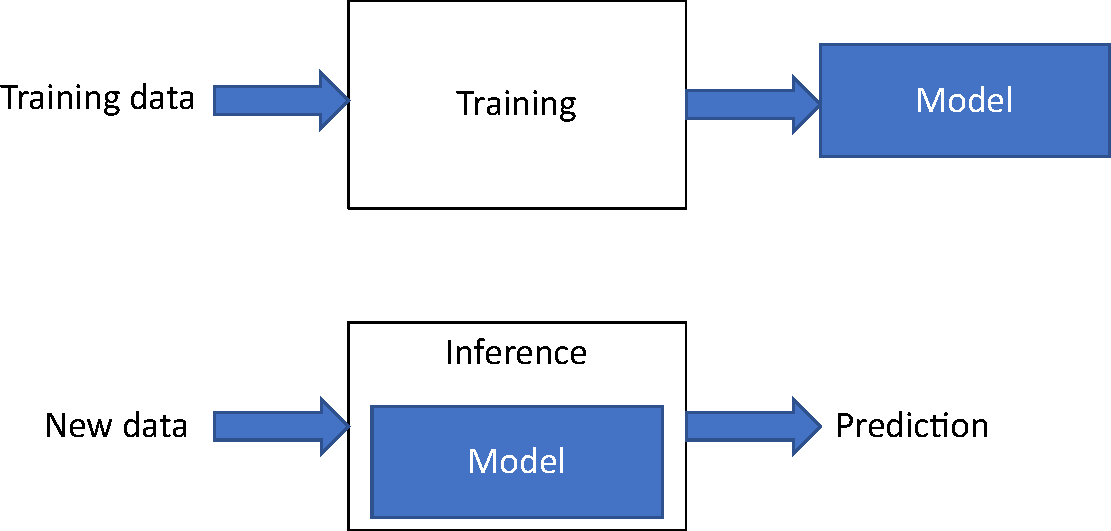
\includegraphics[width=\textwidth]{traininf.pdf}
    \caption{\acrshort{cnn} execution phases, inspired by \cite{nurvitadhi_can_2017}}
    \label{fig:traininf}
\end{figure}

The inference can be accelerated using various optimizations. According to \textcite{abdelouahab_accelerating_2018}, these optimizations can be grouped into 3 main categories:
\begin{itemize}
    \item \textbf{Algorithmic Optimizations}: the computational complexity of \acrshort{cnn}s can be reduced by vectorizing the operations or using faster algorithms.
    \item \textbf{Datapath Optimization}: because of the limited resources on an FPGA, memory is often the bottleneck, and optimizing the memory management can increase the throughput.
    \item \textbf{\acrshort{cnn} model Optimization}: an important issue of \acrshort{cnn} is their computational complexity and hardware utilization. A solution is to trade accuracy for acceleration by using approximate computing.
\end{itemize}

\textbf{\acrshort{cnn} model Optimization} is going to be the key point of this work because the \acrshort{cnn} size and arithmetic complexity are the major issues when implementing a \acrshort{cnn} on mobile devices \cite{cheng_recent_2018}. One of these optimizations, named weight pruning, consists of removing all unnecessary weights of the network \cite{abdelouahab_accelerating_2018}.

This work focus on weight pruning. The irregular data access and the custom data type of the non-pruned weights show it is suitable to implement pruning on \acrshort{fpga}. Therefore, this work concentrates on building an architecture using pruning on \acrfull{dsc}, an alternative way to perform convolution which uses fewer parameters and has a lesser computational complexity. The objective of this work is then to build an efficient architecture on \acrshort{fpga} implementing a sparse \acrshort{cnn} network using \acrshort{dsc}. To assess the benefits of the proposed pruning, we have chosen MobileNetV2 because it offers state of the art performance \cite{sandler_mobilenetv2_2018}.

These work achievements are the following:
%
\begin{itemize}
    \item A structured pruning scheme is proposed to reduce the number of parameters and the computational complexity of the \acrshort{dsc}.
    \item To reduce memory usage, a compressed format is developed to store the non-pruned weights.
    \item An accelerator is designed to support the MobileNetV2 building block performing the sparse \acrshort{dsc}.
    \item The obtained results show that the structured pruning scheme allows a reduction of the computational complexity and the number of parameters, and a faster inference by reducing the latency to execute the \acrshort{dsc}.
\end{itemize}
%
%
\section*{Structure of the thesis}
\addcontentsline{toc}{section}{Structure of the thesis}
%
%
This master thesis is composed of 3 chapters.

Chapter \ref{chap:background} details the background information about the two main topics of this thesis: \acrshort{cnn} and \acrshort{fpga}. First, we explore the theory behind \acrshort{cnn} and go deeper into its computational background in Section \ref{sec:cnn}. Then, the concept and workflow of \acrshort{fpga} are explained in Section \ref{sec:fpga}.

Using knowledge of Chapter \ref{chap:background}, we explore in Chapter \ref{chap:sota} the state of the art techniques on accelerating the inference on \acrshort{fpga}. We explore algorithmic and model optimizations to reduce the cost of the convolution operation and the size of the models. The chapter also details datapath optimizations which reduce the inefficiency of the convolution on \acrshort{fpga}. We also review various \acrshort{fpga} architectures implementing \acrshort{dsc} and pruning of standard convolution.

Chapter \ref{chap:pratique} uses the knowledge from Chapter \ref{chap:sota} to design an efficient architecture using pruning and depthwise separable convolution. It also details the experimental setup to measure the performance of the developed architecture and discusses the obtained results.

Finally, the outcome of this work is shown in the Conclusion. A discussion on the methodology and future works is also presented.
\newpage

	
	%% Part 1
	% Cnn
    \section{Convolutional Neural Network} \label{sec:cnn}
\acrshort{cnn} is a type of \acrshort{nn} specialized in analyzing visual imagery and natural language processing. \acrshort{cnn}s are feedforward, sparsely connected \acrshort{nn}s, and structured as a pipeline of layers \cite{abdelouahab_accelerating_2018}. It showed superior performances in different competitions related to Computer Vision and Image Processing \cite{khan_survey_2020}. Nowadays, \acrshort{cnn}s are used in character and gesture recognition, video classification, face detection, etc \cite{shawahna_fpga-based_2019}. This section aims at investigating the different aspects of a \acrshort{cnn}.

First, the building blocks of a CNN are developed in Section \ref{subsec:layer} starting from its basic element, the \textit{perceptron}. Then, we describe how to use multiple perceptrons to build layers that can perform complex functions. Finally, we detail the other types of layers required to improve the efficiency of the model, such as the pooling layer.

Then, Section \ref{subsec:models} describes how to effectively combine these layers with a focus on the state-of-the-art networks like AlexNet, VGG16, ResNet, and MobileNetV2.

Finally, Section \ref{subsec:train} focuses on the training of \acrshort{cnn}. We briefly explain the back-propagation algorithm, which consists of a forward-propagation and a back-propagation.
%
%
\subsection{Structure of a CNN} \label{subsec:layer}
%
\acrshort{cnn} is a pipeline of layers that can be stacked to form a network \cite{abdelouahab_accelerating_2018}. A layer is a high-level building block, which consists of a set of operations, weights, and non-linear functions. The output of one layer can be used as input of the next layer or as the final output of the network. 

This section first introduces the simplest building element of a \acrshort{cnn}: the perceptron. We describe its different components and notably its activation function. Then, we can use this element to build more complex layers such as the fully connected and convolutional layer. Finally, we present the pooling layer which is used to reduce the spatial dimensions of the output of the previous layer.
%
%
\subsection{Perceptron} \label{subs:perceptron}
The perceptron was developed in 1957 by \textcite{rosenblatt_perceptron_1958}. The idea is to compare the computational model to a human brain which is composed of a large number of units called neurons. A neuron receives an information and when its threshold is reached (we say the neuron fires), this information is released and transmitted to other neurons \cite{rosenblatt_perceptron_1958, matteucci_artificial_2019}.

\begin{figure}
    \centering
    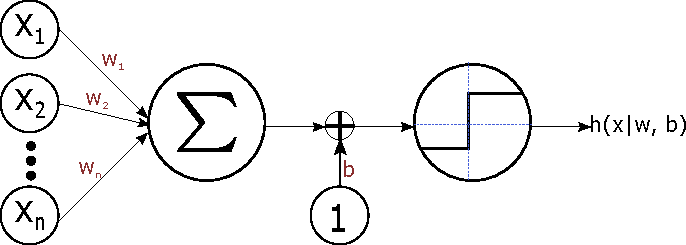
\includegraphics[width=0.8\textwidth]{perceptron.pdf}
    \caption{The Perceptron}
    \label{fig:perceptron}
\end{figure}
%
This neuron in a human brain corresponds to a perceptron in the computational model. It is composed of $n_{in}$ inputs $\boldsymbol{x} = \{ x_1, ... x_{n_{in}} \}$, $n_{in}$ weights $\boldsymbol{w}$ and a bias $b$. Figure \ref{fig:perceptron} illustrates the working principle of a perceptron. When a perceptron received an input vector $\boldsymbol{x}$, a weighted sum of this vector is performed. If its result is higher than the threshold (controlled by $b$), the perceptron is \textquote{activated} and its output becomes a non-zero value.
Equation \ref{eq:perceptron} represents the mathematical formula of the perceptron where $h$ is the activation function of the formula developed in Equation \ref{eq:step} \cite{matteucci_artificial_2019}.
%
\begin{equation}
    h ( \boldsymbol{x} | \boldsymbol{w}, b) = h \left( \sum^{n_{in}}_{i=1} x_i \cdot w_i + b \right) = h \left( \boldsymbol{w}^{T} \cdot \boldsymbol{x} + b \right)
    \label{eq:perceptron}
\end{equation}
%
\begin{equation}
    h ( \boldsymbol{w}^{T} \cdot \boldsymbol{x} + b) = \begin{cases} 1, & \mbox{if } \boldsymbol{w}^{T} \cdot \boldsymbol{x} + b > 0 \\ 0, & \mbox{Otherwise} \end{cases}
    \label{eq:step}
\end{equation}

As the perceptron performs a weighted sum, those weights can be learned to perform a task of interest. However, this model is limited by the functions it can achieve. In Section \ref{subs:fcl}, we discover how we can use multiple perceptrons to create a \textbf{fully-connected layer} to learn more complex functions.

%
\subsection{Activation of a perceptron} \label{subs:acti}
In order to decide if a perceptron is activated or not (if its threshold is reached), an activation function needs to be defined. However, to use this function in a \acrshort{dl} model and be able to apply the back-propagation algorithm (will be further detailed in Section \ref{sec:train}), this function needs to be differentiable \cite{lecun_backpropagation_1989}. Indeed, during the optimization of the network, the gradient of the activation function is computed. Therefore, Equation \ref{eq:step} cannot be used as the activation function because of its zero gradient and the learning does not converge.  Various activation functions have been proposed with different properties, as illustrated in Figure \ref{fig:acti}. According to \textcite{khan_survey_2020}, the choice of an appropriate activation function can accelerate the learning phase and some activations decrease the computational complexity \cite{krizhevsky_imagenet_2012}.
%
\begin{figure}
    \centering
    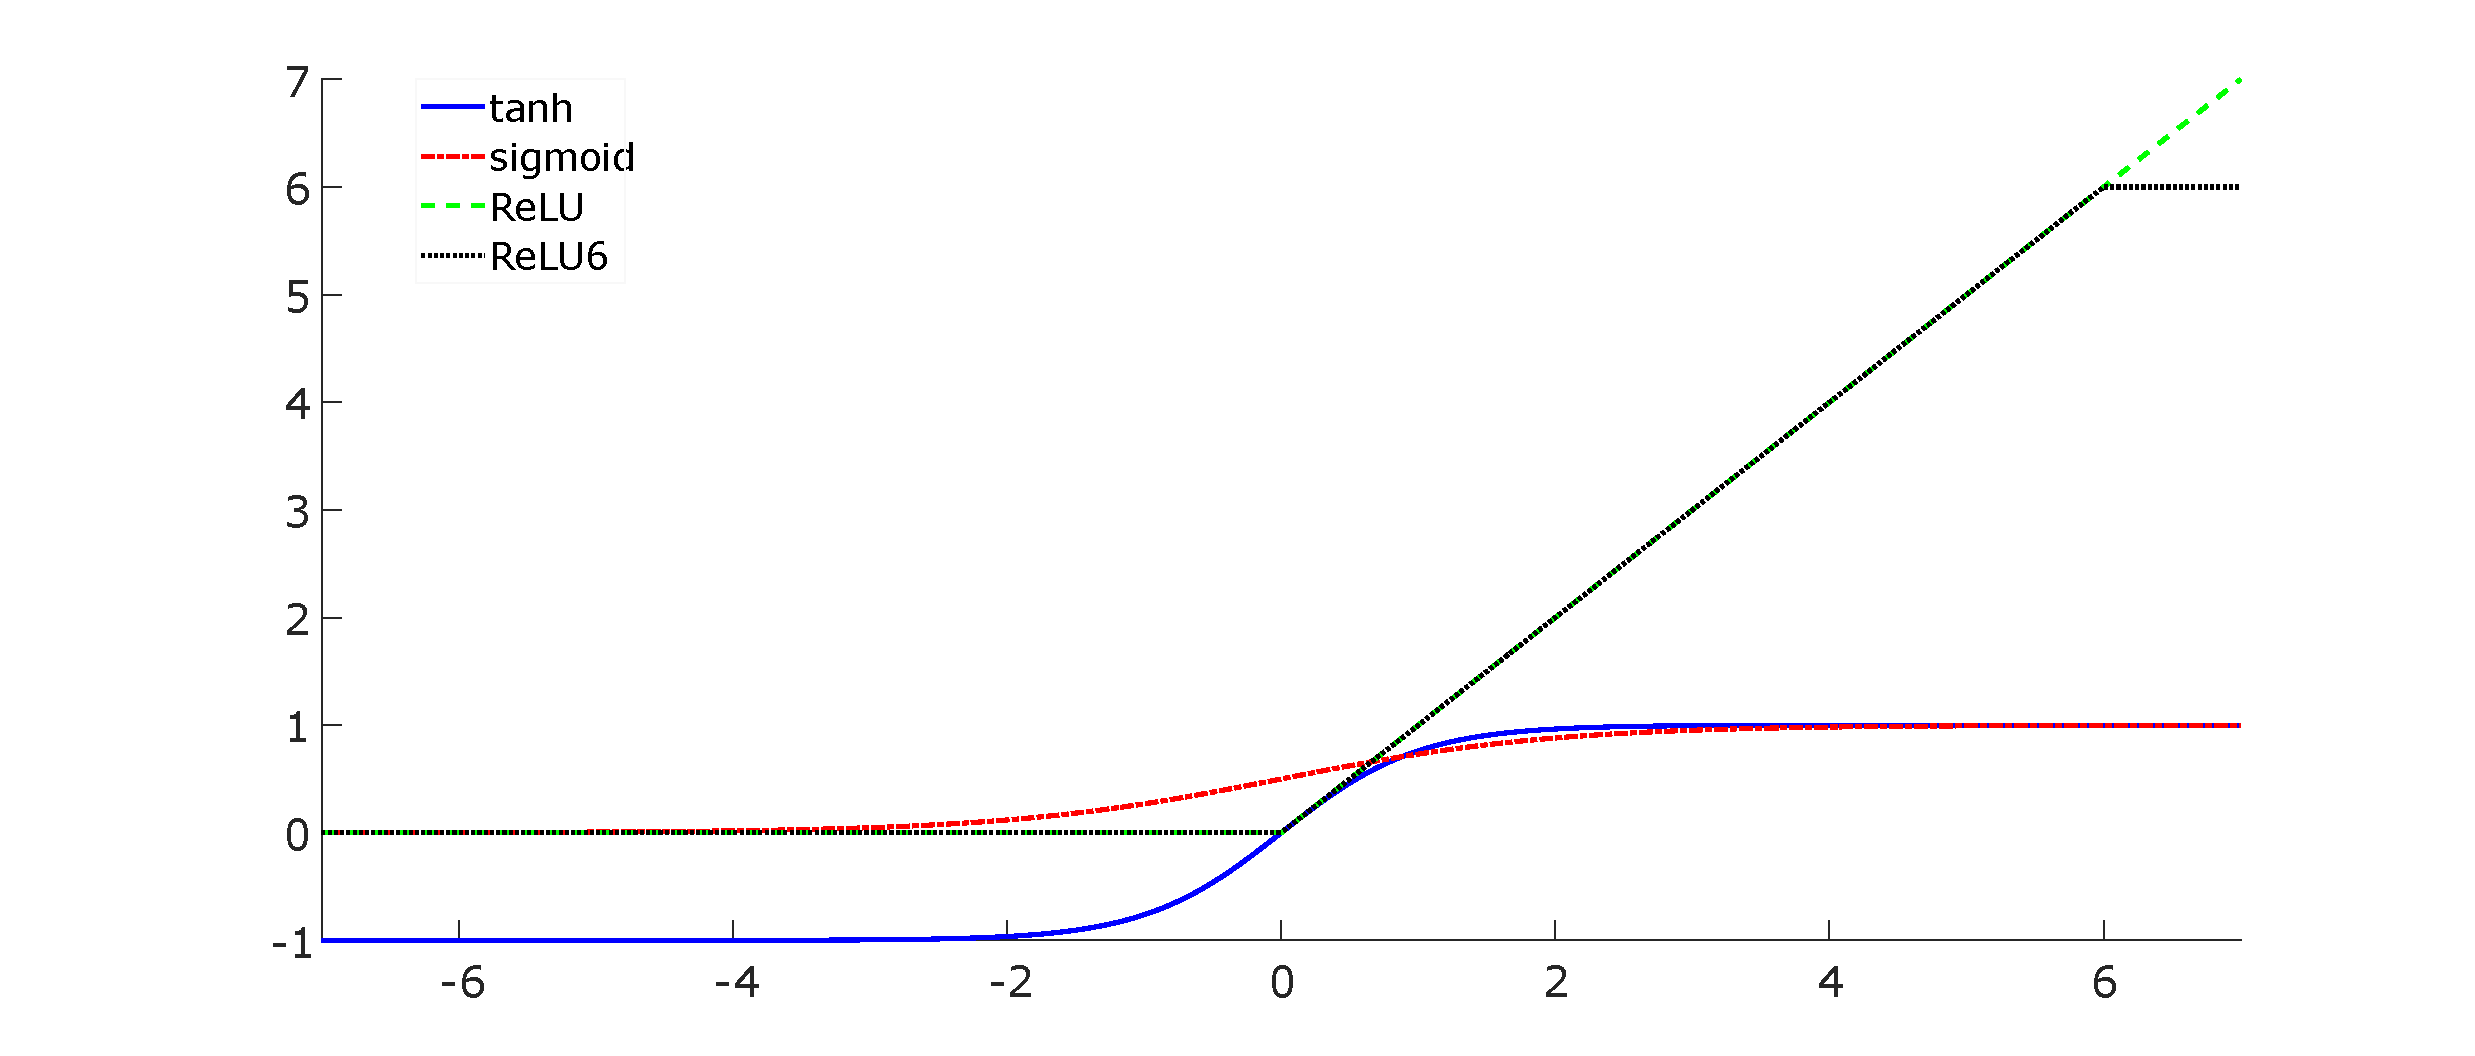
\includegraphics[width=\textwidth]{actifun.pdf}
    \caption{Activation functions}
    \label{fig:acti}
\end{figure}
%
\subsubsection{Sigmoid and Hyperbolic Tangent (Tanh)}
$Sigmoid$ and $Tanh$ are both smooth functions that can be described by equations \eqref{eq:sigmoid} and \eqref{eq:tanh} \cite{krizhevsky_imagenet_2012}.
%
\begin{equation}
    h(x) = \frac{1}{1 + e^{-x}}
    \label{eq:sigmoid}
\end{equation}
%
\begin{equation}
    h(x) = \frac{e^{x} - e^{-x}}{e^{x} + e^{-x}}
    \label{eq:tanh}
\end{equation}
%
These two activation functions can be seen in Figure \ref{fig:acti}. They both limith the $\mathbb{R}$ domain into a narrower domain, $[0, 1]$ for $Sigmoid$, and $[-1, 1]$ for the $Tanh$. However, they also saturate at the asymptotes, which means that often their gradient is close to 0 \cite{glorot_understanding_2010}. As the back-propagation algorithm (see Section \ref{sec:train}) requires gradient multiplication, gradient far away from the output vanishes (close to 0) and deep models do not learn: it is the \textbf{vanishing gradient problem} \cite{goodfellow_deep_2016, khan_survey_2020, maas_rectier_2014}.
%
\subsubsection{ReLU}
In order to overcome this vanishing gradient problem, the Rectified Linear Unit (ReLU) which is defined by Equation \eqref{eq:relu} has been developed by \textcite{krizhevsky_imagenet_2012}.
%
\begin{equation}
    h(x) = max(0, x)
    \label{eq:relu}
\end{equation}
%
This function increases the learning and computational speed compared to the $Tanh$ and $Sigmoid$ functions and improves the propagation gradient efficiency (to avoid vanishing or exploding gradient) \cite{maas_rectier_2014, abdelouahab_accelerating_2018}. However, in this function, some perceptrons can become inactive which means that their output is zero for all input. It is called the \textbf{dying neuron problem} which decreases the model capacity \cite{matteucci_artificial_2019}. A solution would be to discard these inactive neurons by transforming the ReLU into a leaky ReLU \cite{maas_rectier_2014} activation function for example.

We can also use the dying neuron property to learn sparse features earlier. It has been done by \textcite{krizhevsky_convolutional_nodate} by setting an upper bound to the ReLU output. For example, in the work, the output is described by Equation \eqref{eq:relu6} and this activation function is called ReLU6 because the range is limited to $[0, 6]$. ReLU has also the advantage to be designed for fixed-point operations and quantization approaches (which will be more described in Section \ref{subsec:mdopti}), instead of floating-point operations. Indeed, floating-point operations, especially on \acrshort{fpga}, are less efficient in terms of hardware utilization and power consumption \cite{david_hardware_2007}. It means that if for example the output $ \in [0, 6]$, the number of bits for the integer part can be limited to 3 bits. The accuracy of the model can thus be increased by assigning the other available bits to the decimal part. For example, ReLU6 is used in model that aims mobile and embedded platforms like MobileNet \cite{howard_mobilenets_2017}. In this work, the ReLU6 activation function is used.
%
\begin{equation}
    h(x) = max(0, x, 6)
    \label{eq:relu6}
\end{equation}

%
\subsection{Fully Connected layer} \label{subs:fcl}
The perceptron of section \ref{subs:perceptron} can be considered as a linear classifier for which the decision boundary is the hyperplane, as seen in equation \eqref{eq:linearclassifer}.
%
\begin{equation}
    b + w_1 \cdot x_1 + ... + w_{n_{in}} \cdot x_{n_{in}} = 0
    \label{eq:linearclassifer}
\end{equation}
%
We can understand why the perceptron is limited because it has only a linear decision boundary. For example, we can implement the AND and OR Boolean functions using a perceptron, but it is impossible to learn the XOR function. To have a non-linear model, we must use a topology of perceptrons. The topology is composed of layers of perceptrons, where each layer, in the case of a \acrshort{cnn}, is called a \textbf{fully-connected layer}. We can see an example in figure \ref{fig:fcn}.
%
\begin{figure}
    \centering
    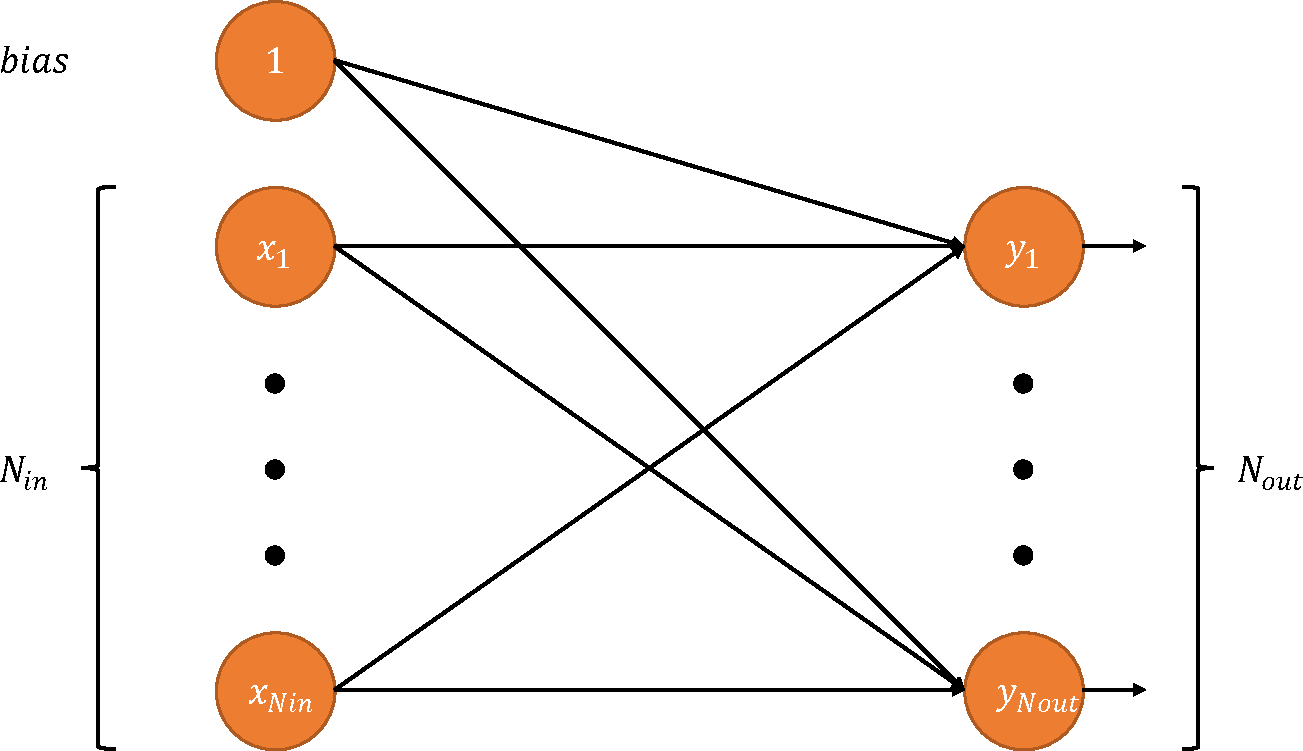
\includegraphics[width=\textwidth]{fcl.pdf}
    \caption{A fully connected layer}
    \label{fig:fcn}
\end{figure}

In the fully-connected layer, each neuron is connected to all the inputs or neurons of previous layers (as the name suggests). Usually, the fully-connected layers are placed at the end of the \acrshort{cnn}. It takes the extracted features from the previous layersas input, which are converted as a one-dimension output \acrshort{fm}. Afterwards, it makes a non-linear classification of them \cite{khan_survey_2020}.

A fully-connected layer is characterized by the number of neurons, activation functions, and the values of weights. The output vector $\boldsymbol{y}$ can be expressed using equation \eqref{eq:fcn}, where $\boldsymbol{x}$ is the vector of the input of the layer and $x_0 = 1$ is the bias;   $\boldsymbol{w}$ is the vector of all the weights of the layer ($w^i_*$ are the weights of the ith perceptron and $w^*_0$ are the biases); $h$ is the activation function of the layer.
%
\begin{equation}
    \boldsymbol{y} = h(\boldsymbol{w}^T \boldsymbol{x}) \Leftrightarrow \forall o \in \{ 1, ..., N_{out} \} : y_o = h(\sum^{N_{in}}_{i=0} w^o_i \cdot x_i)
    \label{eq:fcn}
\end{equation}
%
As we have seen that perceptrons can be used to construct non-linear classifier, we see in the next section \ref{subs:2dconv} the main operation in the \acrshort{cnn}: the \textbf{convolution}, which extracts the feature from input images.

%
\subsection{Convolution layer} \label{subs:2dconv}
In a \acrshort{cnn}, the \textbf{convolutional layer} carries out the feature extraction process of the input image, also called the input \acrfull{fm}. It is the main operation in a \acrshort{cnn} and it is the layer that gives the network its name. The first layer extracts low-level features of the input \acrshort{fm} and the deepest layers use the low-level features to build high-level ones \cite{goodfellow_deep_2016}.

An input image is characterized by 3 parameters: \textbf{$N_{ix}$} the width, \textbf{$N_{iy}$} the height, and \textbf{$N_{if}$} the depth. We can illustrate then the input \acrshort{fm} as a cuboid composed of layers of pixels. An illustration is presented in figure \ref{fig:notation:ifm}.
The convolution layer correlates therefore input \acrshort{fm} and a 4D filter, to produce output \acrshort{fm}, which contains the high-level features \cite{zhao_towards_2018}. The output \acrshort{fm} is also characterized by its width $N_{ox}$, its height $N_{oy}$ and its depth $N_{of}$. We can also see a general output \acrshort{fm} in figure \ref{fig:notation:ofm}. As a result, the filter consists of $N_{of}$ kernels, where each kernel has size $N_{kx} \times N_{ky} \times N_{if}$, that we can see in figure \ref{fig:notation:k}).
%
\begin{figure}
    \centering
    %
    \begin{subfigure}{.32\textwidth}
    \centering
    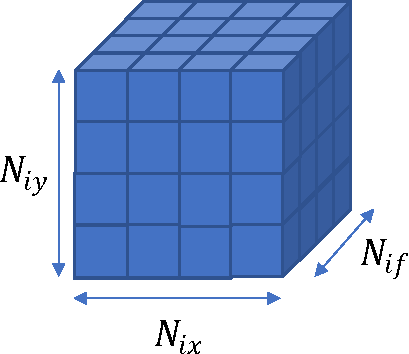
\includegraphics[width=\linewidth]{notifm.pdf}
    \caption{kernel-wise pruning}
    \label{fig:notation:ifm}
    \end{subfigure}
    %
    \begin{subfigure}{.32\textwidth}
    \centering
    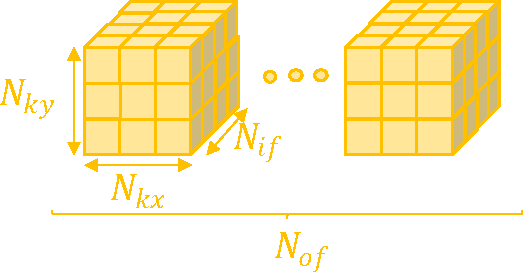
\includegraphics[width=\linewidth]{notk.pdf}
    \caption{Convolution kernel}
    \label{fig:notation:k}
    \end{subfigure}
    %
    \begin{subfigure}{.32\textwidth}
    \centering
    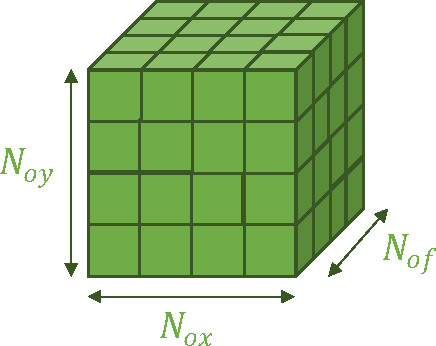
\includegraphics[width=\linewidth]{notofm.pdf}
    \caption{Output \acrshort{fm}s}
    \label{fig:notation:ofm}
    \end{subfigure}
    %
    \caption{Volumes involved in the convolution operations}
    \label{fig:notconv}
\end{figure}

Convolution is a specialized kind of linear operation. The convolution operation happens as follows. Each kernel acts like a sliding window on the input \acrshort{fm}. We extract a chunk of pixels of the same size of the kernel in the input \acrshort{fm} and perform an element-wise multiplication with the chunk of data and the kernel. We sum up the computed pixels to obtain one output pixel. Sliding this kernel on the input \acrshort{fm} will produce a channel of the output \acrshort{fm}, where the output pixel at position $(x, y)$ corresponds to the movement of the sliding window from the top left of the input \acrshort{fm}. Since one kernel produces one channel of the output \acrshort{fm}, having $N_{of}$ kernels produces then $N_{of}$ channels. An illustration of the convolution operation is in figure \ref{fig:convolution}.
%
\begin{figure}
    \centering
    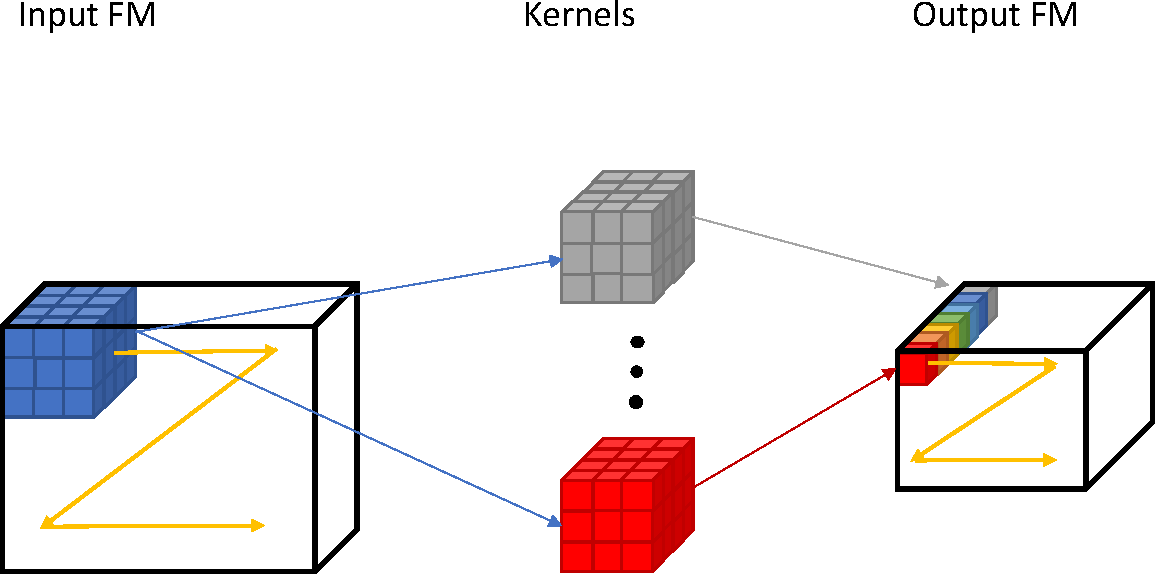
\includegraphics[width=\textwidth]{conv.pdf}
    \caption{Convolution operation}
    \label{fig:convolution}
\end{figure}

Except for $1 \times 1$ kernels, the sliding window can not cover all input pixels, and then there is a spatial reduction between the input and output \acrshort{fm}s, while there is an increase in the number of channel. However, we can keep the same dimensions using \textit{padding} on the boundary. It means that we pad the edges with extra pixels (usually of value 0).

Moreover, each time the sliding window performs a convolution, it shifts in the input \acrshort{fm}. The amount, by which the filter shifts, is called the \textit{stride} and it is initially set to 1. If we increase the stride, we can reduce the spatial dimensions of the output \acrshort{fm}. For example, if we use padding and a stride of 2, $\frac{N_{ix}}{N_{ox}} = \frac{N_{iy}}{N_{oy}} = \frac{1}{2}$, and the output \acrshort{fm} has 4 times fewer pixels. In section \ref{subs:pooling}, we introduce a new layer than can also reduce the spatial dimensions of the output \acrshort{fm}.

Finally, we can express the convolution operations mathematically as in equation \eqref{eq:conv}.
%
\begin{equation}
    \begin{split}
        \forall ox &\in \{ 1, ..., N_{ox} \}, oy \in \{ 1, ..., N_{oy} \}, of \in \{ 1, ..., N_{of} \} : \\
        FM_O[ox, oy, oc] &= \sum^{N_{if}}_{if=1}
        \sum^{N_{kx}}_{kx=1}
        \sum^{N_{ky}}_{ky=1}
        FM_I[ox \cdot S + kx - \lfloor \frac{N_{kx}}{2} \rfloor,  oy \cdot S + ky - \lfloor \frac{N_{ky}}{2} \rfloor, if] \cdot
        W^{of}_{if}[kx, ky]
    \end{split}
    \label{eq:conv}
\end{equation}

If we compare the convolutional layer with the fully-connected layer, the convolutional layer allows a sparse interaction (the kernel is smaller than the input), parameter sharing (we use the same parameter for more than one function) and equivariant representation (for some transformation, a change in the input reflects the same change in the output) \cite{goodfellow_deep_2016}. To illustrate weight sharing, in AlexNet \cite{krizhevsky_imagenet_2012}, 94\% of the weights are used in the fully-connected layers. But as said earlier, convolution is a computationally heavy operation. 90\% of the arithmetic operations are done in the convolutional layer.

As the convolution has a huge arithmetic complexity, we see in the following section \ref{subs:dsc} an alternate way to perform convolution to reduce this.

%
\subsubsection{Depthwise Separable Convolution}  \label{subs:dsc}
\acrfull{dsc} was first introduced by \textcite{sifre_ecole_2014}. According to \textcite{chollet_xception_2017}, \textquote{\textit{A depthwise separable convolution consists in a \textbf{depthwise convolution}, i.e. a spatial convolution performed independently over each channel of an input, followed by a \textbf{pointwise convolution}, i.e. a $1 \times 1$ convolution, projecting the channel's output by the depthwise convolution onto a new channel space}}.

It means that the \acrshort{dsc} is composed of a depthwise convolution followed by a pointwise convolution as illustrated in Figure \ref{fig:dsc}. This alternative form of convolution has been developed to reduce efficiently the arithmetic complexity, in exchange of a limited loss of accuracy \cite{liu_fpga-based_2019}. As a result, the \acrshort{dsc} has significantly fewer parameters and operations with respect to the standard convolution. Equations \eqref{eq:descopred} and \eqref{eq:descwgred} are used to calculate the reduction factors on weigths and on operations respectively, where $F_{*}$ are the factors of reduction, $W_{sc}$ and $O_{sc}$ are the weights and operations required for a standard convolution, and $W_{dsc}$ and $O_{dsc}$ are the weights and operations required for a \acrshort{dsc} \cite{liu_fpga-based_2019}.
%
\begin{equation}
    F_w = \frac{W_{dsc}}{W_{sc}} =
    \frac{N_{kx} \times N_{ky} \times N_{if} + N_{if} \times N_{of}}{N_{kx} \times N_{ky} \times N_{if} \times N_{of}} =
    \frac{1}{N_{of}} + \frac{1}{N_{kx} \times N_{ky}}
    \label{eq:descopred}
\end{equation}
\begin{equation}
    \begin{split}
        F_o &= \frac{O_{dsc}}{O_{sc}} = \frac{N_{kx} \times N_{ky} \times N_{if} \times N_{ox} \times N_{oy} + N_{if} \times N_{of} \times N_{ox} \times N_{oy}}{N_{kx} \times N_{ky} \times N_{if} \times N_{of} \times N_{ox} \times N_{oy}} \\
        &= \frac{1}{N_{of}} + \frac{1}{N_{kx} \times N_{ky}}
    \end{split}
    \label{eq:descwgred}
\end{equation}

Using equation \eqref{eq:descopred} and equation \eqref{eq:descwgred} and $3 \times 3$ kernels, the reduction of computation and parameters in comparison with the standard convolution is about 9 times \cite{zhang_channel_2019}.
%
\begin{figure}
    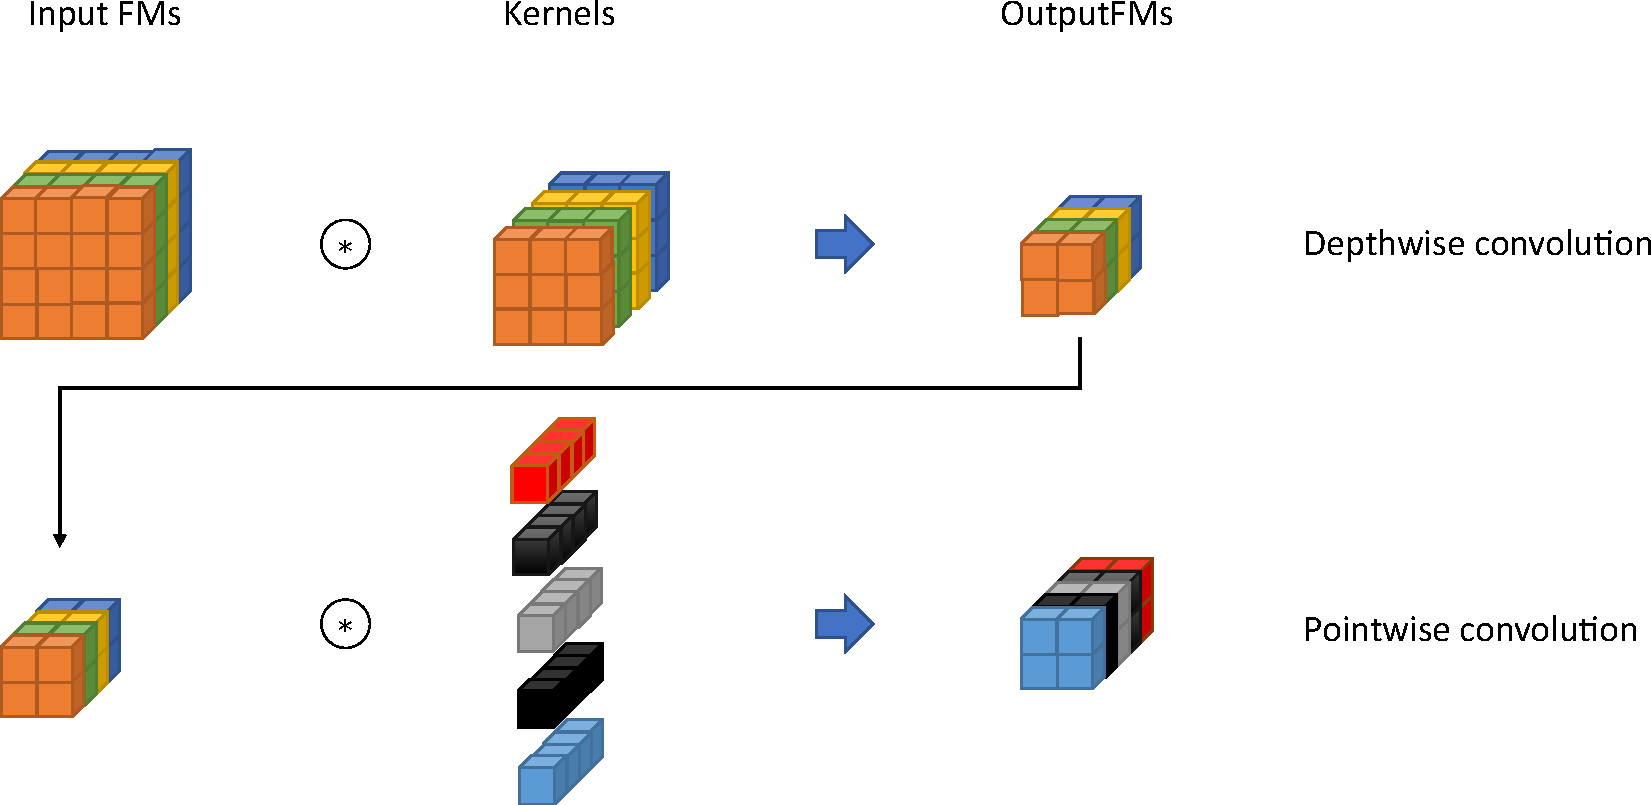
\includegraphics[width=\textwidth]{dsc.pdf}
    \caption{Depthwise Separable Convolution}
    \label{fig:dsc}
\end{figure}

%
\subsubsection{Pooling} \label{subs:pooling}
A Pooling layer is used to replace the output of the previous layer by a summary statistics of this output \cite{goodfellow_deep_2016}. They are usually inserted between the successive convolutional layer to modify the output further. Its goal is first to make the output approximately invariant to small translations and it also reduces the spatial size of each output \acrshort{fm}. It means that the memory needed to store the parameters is reduced \cite{goodfellow_deep_2016}. It also reduces the number of parameters and the computation of the network while also increasing the receptive field \cite{shawahna_fpga-based_2019}.

The pooling layer divides each \acrshort{fm} into regions of size $K \title K$ and outputs one pixel from each region. This way, is kept constant while their spatial size is reduced by $K$. Various pooling functions exist, but the most common form uses filters of size $2 \times 2$ where for example the MAX or AVG operation selects the highest pixel from 4 samples their average respectively (meaning a 75\% reduction of the pixels) \cite{suda_throughput-optimized_2016}. Figure \ref{fig:pool} illustrates an example of a pooling layer.
%
\begin{figure}
    \centering
    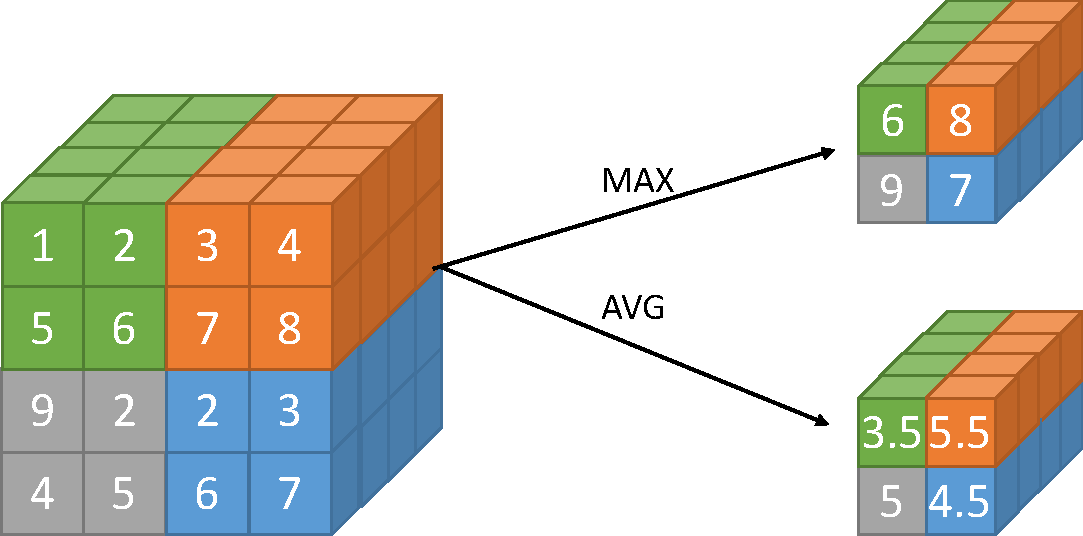
\includegraphics[width=0.8\textwidth]{pooling.pdf}
    \caption{An example of pooling layers}
    \label{fig:pool}
\end{figure}

%
\subsubsection{Summary}
%
The summary of this section is provided in Figure \ref{fig:layer:summary}. First, an input image is fed to the \acrshort{cnn}. Then, three different kinds of layers can be used:
%
\begin{enumerate}
    \item \textbf{The convolutional layer}, which extracts the features from the input.
    \item \textbf{The pooling layers}, which summarizes the output of the previous layer.
    \item \textbf{The fully connected layer}, which is a non-linear classifier.
\end{enumerate}
%
A typical \acrshort{cnn} is composed of two parts, which are built from stacking the previously mentioned layers \cite{matteucci_artificial_2019}:
\begin{enumerate}
    \item \textbf{The feature extractor} part, composed of blocks made of convolutional, activation, and pooling layers.
    \item \textbf{The classifier} part, composed only of fully connected layers.
\end{enumerate}
%
\begin{figure}[H]
    \centering
    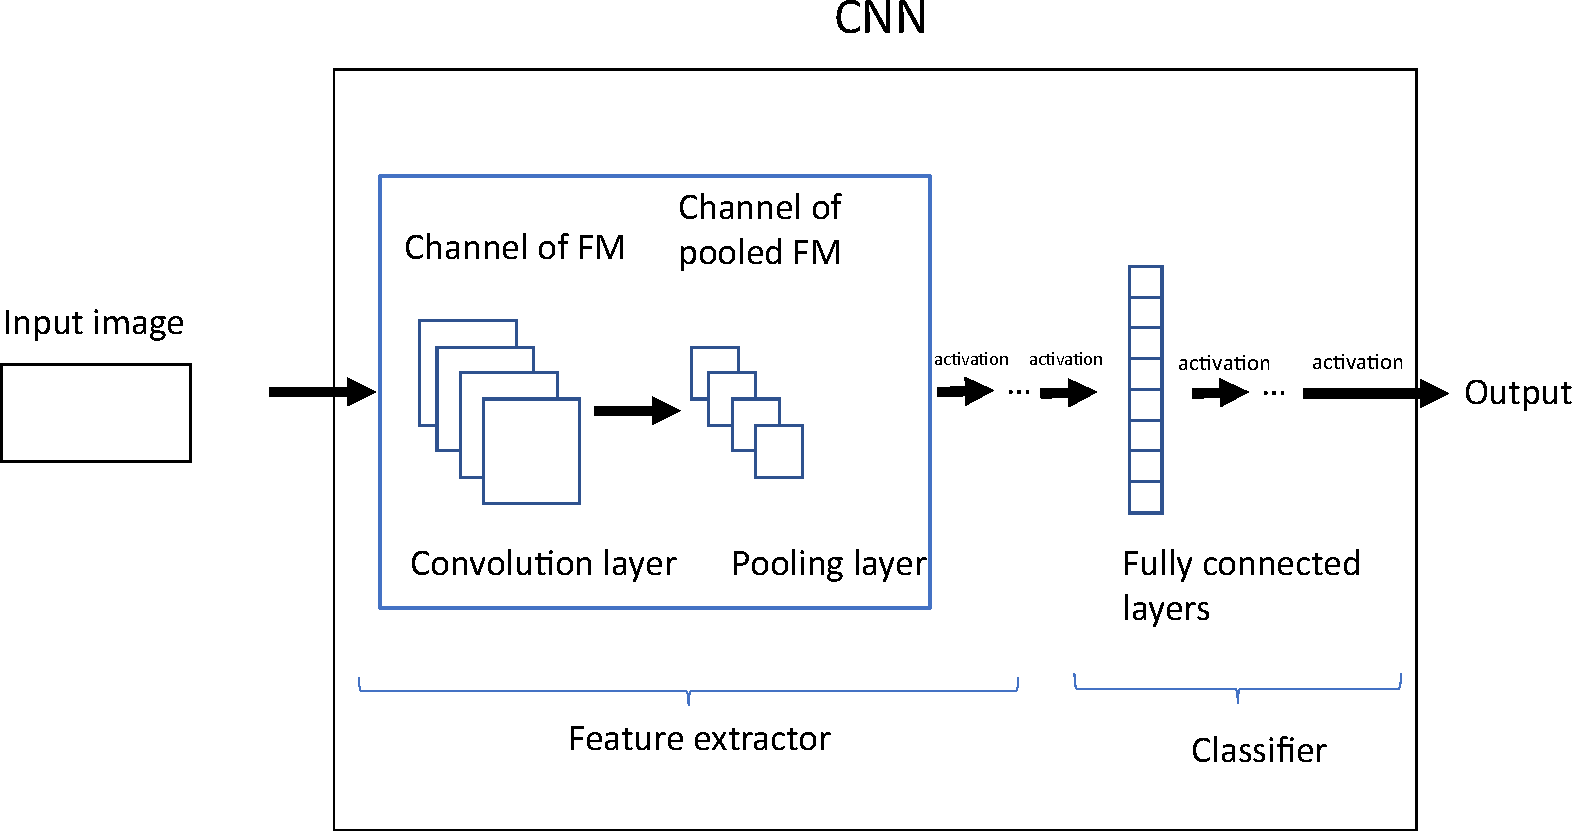
\includegraphics[width=0.75\textwidth]{cnn_summary.pdf}
    \caption{Working principle of a CNN and the different layers which composing it}
    \label{fig:layer:summary}
\end{figure}
%
\subsection{CNN Models} \label{subsec:models}
After the analysis of the CNN structure in Section \ref{subsec:layer}, this section details some of the well-known \acrshort{cnn} networks. They are examples of how to construct an efficient \acrshort{cnn}.

%
\subsubsection{AlexNet}
%
AlexNet is a famous \acrshort{cnn} which was developed in 2012 by \textcite{krizhevsky_imagenet_2012}. It is a breakthrough in the deep \acrshort{cnn} field and this model won the ImageNet competition. Krizhevsky et al. used some parameters optimizations and made the model deeper in order to considerably improve the learning ability of the CNN \cite{khan_survey_2020}. It is composed of 5 convolutional layers and 3 fully-connected layers, as seen in Figure \ref{fig:alexnet}. Each convolutional layer has a ReLU activation function and it uses pooling.
%
\begin{figure}[H]
    \centering
    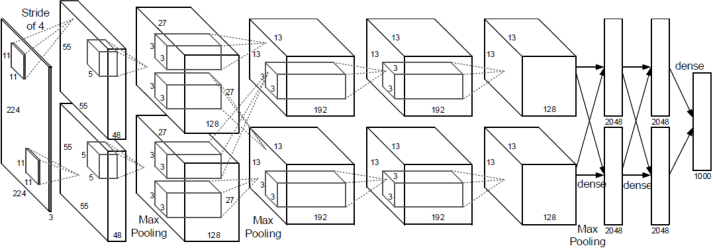
\includegraphics[width=\textwidth]{alexnet.pdf}
    \caption{An illustration of the architecture of AlexNet \cite{krizhevsky_imagenet_2012}}
    \label{fig:alexnet}
\end{figure}
%
\subsubsection{VGG}
%
After the success of AlexNet in 2012, research was made to reduce the computational complexity while keeping the accuracy. In 2014, VGG, a deeper variant of AlexNet was developed by \textcite{simonyan_very_2015}. It is composed of 5 groups of convolutional layers, where the number of layers depends on the version of VGG. It won the localization in the ImageNet challenge in 2014 \cite{simonyan_very_2015}. An illustration is provided by Figure \ref{fig:vgg}. This level of depth was possible thanks to the application of very small ($3 \times 3$) convolution kernels. They allow a larger receptive field with fewer parameters and more non-linearities than a larger kernel. However, it has a high memory request. 100MB per image needs to be stored in all \acrshort{fm}s for the forward propagation \cite{matteucci_artificial_2019}.
%
\begin{figure}[H]
    \centering
    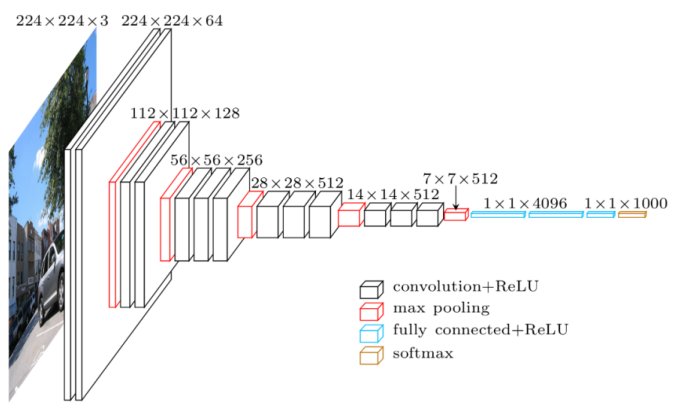
\includegraphics[width=0.75\textwidth]{VGG.pdf}
    \caption{An illustration of the architecture of VGG16 \cite{simonyan_very_2015}}
    \label{fig:vgg}
\end{figure}
%
\subsubsection{ResNet}
%
\textcite{he_deep_2016} developed ResNet in 2015. It is a very deep network which can contain from 50 to 1000 convolutional layers. It is composed of structures which are more complex and irregular than in the networks described previously. \textcite{he_deep_2016} showed that an increase of the depth of the network does not leads to an improvement of the performance. Indeed, beyond a certain amount of layers, a continuous increase of the depth leads to the degradation of the accuracy. This is not due to overfitting. It is because the deeper models are harder to optimize than shallower ones (vanishing gradient described in Section \ref{subs:trainbackward}) \cite{matteucci_artificial_2019}. 

However, deeper networks should at least have similar or better performance than shallower ones. Indeed, let’s compare a deeper and a shallower network. If the deeper network is composed of the same layers than the shallower one and that the other added layers are just identity mapping, then the network should have the same performance than the shallower one. Therefore, a deeper network should not have worse performance than shallower ones \cite{matteucci_artificial_2019}.

To overcome this issue, \textcite{he_deep_2016} introduced an \textit{identity shortcut connection} which skips one or more layers and set weights to the identity, as can be seen in Figure \ref{fig:resnet}. These weights associated to the shortcut connection can be used to learn a residual $\mathcal{F}(x)$ in order to improve the solution. The performance of this very deep network allowed it to win the 2015 ILSVR for both localization and classification.
%
\begin{figure}[H]
    \centering
    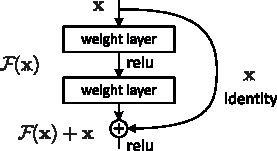
\includegraphics[width=0.7\textwidth]{resnet.pdf}
    \caption{ResNet building block, from \cite{he_deep_2016}}
    \label{fig:resnet}
\end{figure}
%
\subsubsection{MobileNetV2} \label{subs:mbv2}
%
According to \textcite{cheng_recent_2018}, the performance of \acrshort{cnn} in recent years became outstanding. These improvements came at the cost of storage and computational complexity. It is not an issue for the \acrshort{cnn} training phase, because the GPU and CPU also gained in computational units and memory. However, for the inference phase, the computational complexity and the storage requirements are way beyond the capabilities of most of the embedded applications and mobile devices such \acrshort{fpga} \cite{cheng_recent_2018}.
%
\begin{itemize}
    \item The enormous computational complexity of \acrshort{cnn}s makes it difficult to deploy on real-time applications and it consumes battery power.
    \item The large number of parameters of \acrshort{cnn}s consumes considerable storage and run-time memory.
\end{itemize}

In order to overcome this issue, \textcite{sandler_mobilenetv2_2018} introduced a network called MobileNetV2 in 2018. It is specifically developed for constrained environments. First, the size and number of operations is decreased thanks to DSC (see Section \ref{subs:dsc}) and thanks to a new type of layer \textit{inverted residual with a linear bottleneck}, which can be observed in Figure \ref{fig:invreslinbot} and Table \ref{tab:invreslinbot}.
This layer is composed of a $1 \times 1$ convolution to expand the number of the input \acrshort{fm} channels by a factor $t$ ($N_{intf} = t \times N_{if}$). It is then followed by a \acrshort{dsc}. The purpose of the first convolution layer which increases the number of channels is supposed to counterbalance the loss of information that occurred by the ReLU activation. They also added a skip connection to build a network of great depth, and the last convolution has a linear activation function \cite{sandler_mobilenetv2_2018}.
%
\begin{figure}[H]
    \centering
    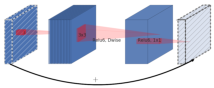
\includegraphics[width=\textwidth]{mbnv2.pdf}
    \caption{inverted residual with linear bottleneck \cite{sandler_mobilenetv2_2018}}
    \label{fig:invreslinbot}
\end{figure}
%
\begin{table}
    \center
    \begin{tabular}{c|c|c}
        Input & Operetor & Output \\
        \hline \hline
        $N_{ix} \times N_{iy} \times N_{if}$ & $1 \times 1$ conv2d, ReLU6 & $N_{ix} \times N_{iy} \times (t \times N_{if})$ \\
        $N_{ix} \times N_{iy} \times (t \times N_{if})$ & $3 \times3$ dwise s=$s$, ReLU6 & $\frac{N_{ix}}{s} \times \frac{N_{iy}}{s} \times (t \times N_{if})$ \\
        $\frac{N_{ix}}{s} \times \frac{N_{iy}}{s} \times (t \times N_{if})$ & $1 \times 1$ conv2d & $\frac{N_{ix}}{s} \times \frac{N_{iy}}{s} \times N_{of}$ \\
        \hline \hline
    \end{tabular}
    \caption{inverted residual with linear bottleneck \cite{sandler_mobilenetv2_2018}}
    \label{tab:invreslinbot}
\end{table}

More information about the structure of MobileNetV2 can be found in Appendix \ref{appendix:mbv2}.

%
%
\subsection{Training} \label{subsec:train}
The previous section described the common building blocks present in \acrshort{cnn}s and how to design a \acrshort{cnn}. This section aims at detailing how a network improves automatically its performance for a specific task. This is called \textit{learning}.

The learning phase starts after designing the network. However, before the model can learn, we have to initialize the weights. The most common initialization is a random Gaussian distribution \cite{he_delving_2015}. However, the learning phase is affected by the initial values of the weights. If it is too small the network does not learn or if it is too large it might take a very long time to converge. Different initializations were suggested to improve the learning phase: Xavier initialization \cite{glorot_understanding_2010} and He initialization \cite{he_delving_2015}.

When values are assigned to the weights, the back-propagation algorithm can be performed to improve the efficiency of the network. The back-propagation algorithm is composed of two steps: the forward-propagation and the back-propagation. In the following sections, we briefly review each of them.
%
\subsubsection{Forward-propagation} \label{subs:trainforward}
%
The first step of the backpropagation algorithm is the forward propagation. During this step, the training data are used as input of the model and each input is propagated through the network using the initialized weights. A vector of outputs is produced and is compared using a loss function (for example mean-square error defined by Equation \eqref{eq:mse}) with the label of the input (target $\boldsymbol{t}$) \cite{matteucci_artificial_2019}. The weights are then adjusted in order minimize the loss function. This can be done using the algorithms found in the next section. When the model is trained, the inference consists only of the forward propagation \cite{abdelouahab_accelerating_2018}.
%
\begin{equation}
    L(\boldsymbol{x}, \boldsymbol{w}) = \sum^{N}_{i=1} (t_i - p(x_i, \boldsymbol{w}))^2
    \label{eq:mse}
\end{equation}

%
\subsection{Back-propagation} \label{subs:trainbackward}
According to \textcite{ruder_overview_2017}, gradient descent optimization algorithms are the most popular to perform optimizations on \acrshort{nn}. These algorithms derive from the idea of gradient descent. As said in the previous section, gradient descent is a way to minimize the loss function, parametrized by the model's parameters (weight). We can, therefore, describe gradient descent algorithm using equation \eqref{eq:gd}, where $\eta$ is the learning rate, a positive scalar determining the size of the step in the direction minimizing the gradient \cite{goodfellow_deep_2016}. If we update the weight in the opposite direction of the gradient, we can reach a local minimum.
%
\begin{equation}
    \boldsymbol{w} = \boldsymbol{w} - \eta \frac{ \partial L( \boldsymbol{x}, \boldsymbol{w} ) }{\partial \boldsymbol{w}}
    \label{eq:gd}
\end{equation}

\textbf{The original gradient descent} or \textbf{batch gradient descent }computes the gradient using the whole dataset (the batch). We see how to compute the gradient on equation \eqref{eq:gd-grad}. This might be impossible to do in practice if the dataset is too large. Variations have then be proposed to make the gradient descent to be practical.
%
\begin{equation}
    \frac{ \partial L( \boldsymbol{x}, \boldsymbol{w} ) }{\partial \boldsymbol{w}} = \frac{1}{Nin} \sum^{Nin}_{i = 0} \frac{ \partial L( x_i, \boldsymbol{w} ) }{\partial \boldsymbol{w}}
    \label{eq:gd-grad}
\end{equation}

\textbf{Stochastic gradient descent}, instead of using the entire dataset, performs the gradient descent algorithm on one sample at a time. We see how to compute the gradient on equation \eqref{eq:sgd-grad}. It avoids the redundant computation of the batch gradient descent. It learns faster and can reach better local minima, however, it is complicated to find the global minimum.
%
\begin{equation}
    \frac{ \partial L( \boldsymbol{x}, \boldsymbol{w} ) }{\partial \boldsymbol{w}} = \frac{ \partial L( x_i, \boldsymbol{w} ) }{\partial \boldsymbol{w}}
    \label{eq:sgd-grad}
\end{equation}

\textbf{Mini-batch gradient descent} is a trade-off between the two approaches. It performs an update of the weight for every mini-batch of $N$ training examples. It has better convergence  by reducing the variance and has less computation than batch gradient descent.
%
\begin{equation}
    \frac{ \partial L( \boldsymbol{x}, \boldsymbol{w} ) }{\partial \boldsymbol{w}} = \frac{1}{N} \sum^{N < Nin}_{i = 0} \frac{ \partial L( x_i, \boldsymbol{w} ) }{\partial \boldsymbol{w}}
    \label{eq:bgd-grad}
\end{equation}

%
%

    \afterpage{\blankpage}
    \cleardoublepage
    \newpage
% FPGA
    \chapter{FPGA}
\label{chap:fpga}
\section{Loop optimization techniques} \label{sec:loopopti}
\acrfull{simd} accelerators were proposed to solve the static systolic array inefficiency. The general computation flow can be described as follow:
\begin{enumerate}
    \item Fetch \acrshort{fm}s and weights from the external memory (\acrshort{dram}) to on-chip buffer.
    \item The \acrshort{fm}s and weights are streamed into the \acrshort{pe}.
    \item
\end{enumerate}

    \afterpage{\blankpage}
    \cleardoublepage
    \newpage

	
	%% Part 2
	\chapter{State of the Art} \label{chap:sota}
Chapter \nameref{chap:background} detailed all the background information required to understand the theory behind \acrshort{cnn} and \acrshort{fpga}. This chapter aims at reviewing the main optimization techniques known in the literature to implement an efficient \acrshort{cnn} accelerator on \acrshort{fpga}, to achieve the objective of this thesis.

Section \ref{sec:opti_cnn} details optimization techniques to modify the computational model of the \acrshort{cnn} allowing an efficient inference on \acrshort{fpga}. Section \ref{subsec:algopti} is focused on reducing the algorithmic complexity of the \acrshort{cnn} by optimizing the convolution operation while Section \ref{subsec:mdopti} covers techniques to trade accuracy for a reduction of the number of parameters and algorithmic complexity.

Section \ref{sec:opti_dataflow} is focused on studying efficient ways to handle a \acrshort{cnn} on \acrshort{fpga}. First, we review how a general \acrshort{cnn} is implemented while reducing inefficiencies. Then, we look at architectures that successfully implement \acrshort{dsc} in Section \ref{subsec:impl_dsc}, and pruning in Section \ref{subsec:impl_prun}.
% inference optimization
\section{CNN optimizations for FPGA} \label{sec:opti_cnn}
%
%
The previous chapter has described the way \acrshort{cnn} work and the different state-of-the-art models. Section \ref{subs:mbv2} evidenced the issue to implement the inference phase on mobile devices such as \acrshort{fpga}. Indeed, the computational complexity and the storage requirements are way beyond their capabilities. This section explores the state-of-the-art approaches to reduce the arithmetic complexity and the hardware utilization to handle this problem on a \acrshort{fpga}. First, Section \ref{subsec:algopti} details how to efficiently handle and optimize the convolution operation on \acrshort{fpga}. Then, Section \ref{subsec:mdopti} covers techniques to reduce the size of the model.
%
\section{Algorithmic Optimizations} \label{sec:algopti}
In this section we will review algorithmic optimization techniques to reduce computational complexity of convolutions, which are a costly operation. According to \cite{shawahna_fpga-based_2019}, 90\% of computation time in \acrshort{cnn} are consummed by the convolution operation.
%
%
\subsection{\acrfull{gemm}}
%
%
It is a common way to process \acrshort{cnn} on \acrshort{cpu} and \acrshort{gpu}. We convert the convolution as a matrix-vector multiplication.  The process of a convolution layer can be observed on Figure \ref{fig:gemm}.
However, this approach is not suggested for \acrshort{fpga}: \cite{sze_efficient_2017, zhu_efficient_2020} point out that the \acrshort{fm}s have to be copied multiple times when flattened to a vector. It leads to a huge memory footprint and either ineffiency in storage or complex memory management access patterns.
\begin{figure}
    \centering
    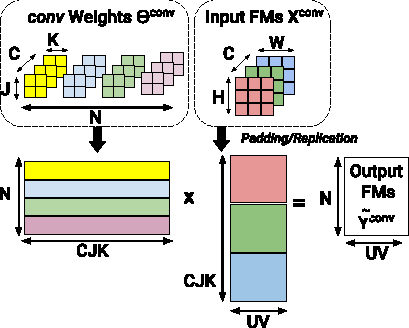
\includegraphics[width=0.5\textwidth]{Images/gemm.pdf}
    \caption{\acrshort{gemm} base processing on conv layer}
    \label{fig:gemm}
\end{figure}
%
%
\subsection{Winograd Transform}
%
%
The Winograd minimal filter algorithm is first introduced by \cite{winograd_arithmetic_1980}. We can apply this computational transform to convolutions when the stride is equal to 1. In Winograd filtering, data is processed by blocs referred as \textit{tiles}, as following:
\begin{itemize}
    \item An input \acrshort{fm} tile $g$ of size $(N_{ix} \times N_{iy})$ is pre-processed: $\tilde{g} = \boldsymbol{G^{T}} g \boldsymbol{G} $, where $\boldsymbol{G}$ is a transformation matrix defined in the Winograd Algorithm \cite{winograd_arithmetic_1980}.
    \item In a same way, $d$, the filter of size $(K_x \times K_y)$ is transformed into $\tilde{d}$: $\tilde{d} = \boldsymbol{B^{T}} d \boldsymbol{B}$ , where $\boldsymbol{B}$ is a transformation matrix defined in the Winograd Algorithm \cite{winograd_arithmetic_1980}.
    \item The output tile $Y$ of the Winograd Filtering algorithm, denoted $F(N_{ix} \times N_{iy}, K_x \times K_y)$ is computed using equation \ref{eqn:winograd}, where $\boldsymbol{A}$ is a transformation matrix defined in the Winograd Algorithm \cite{winograd_arithmetic_1980} and $\odot$ indicates element-wise multiplication.
\end{itemize}
\begin{equation}
\label{eqn:winograd}
Y = \boldsymbol{A^{T}} [ \ \tilde{g} \odot \tilde{d} \ ] \boldsymbol{A}
\end{equation}
\cite{lavin_fast_2015} demonstrated that Winograd convolution is efficient when the kernel is small ($K_* \leq 3$) and the number of multiplication can be reduced by a factor of $2.25 \times$ (in returns the number of addition is increased). According to \cite{sandler_mobilenetv2_2019}, $3 \times 3$ kernel is a standard for modern networks, which leads to think that Winograd Transform is a usefull approach to reduce computational complexity of convolutional layers. For example, \cite{aydonat_opencl_2017, lu_evaluating_2017} utilized Winograd transform and haved reduced their computational complexity by around 50\%.
%
%
\subsection{\acrfull{fft}}
%
%
The \acrshort{fft} is an algorithm to transform the 2D convolution into element-wise multiplication in the frequency domain. The equation is observed at equation \ref{eqn:fft}
\begin{equation}
\label{eqn:fft}
conv2D(FM_{I}[ic], K[oc, ic]) = IFFT( FFT(FM_{I}[ic]) \odot FFT(K[oc, ic]) )
\end{equation}
The arithmetic complexity of the 2D convolution can be reduced to $O(N_{ix}^2 log_2(N_{ix}))$ \cite{jong_hwan_ko_design_2017} and the computational complexity of the \acrshort{fft} can be reduced to $O(N_{ix} log_2(K_{x}))$ using the Overlap-and-Add Method \cite{w_smith_scientist_1997}.
However, the \acrshort{fft} finds its interest when kernel are large \cite{lavin_fast_2015} ($K_* \geq 5$), which is not a standard kernel size according to \cite{sandler_mobilenetv2_2019}. \cite{zhang_frequency_2017} implemented \acrshort{fft} algorithm for \acrshort{cnn} on \acrshort{fpga} and it showed little reduction of computation complexity with small filters such as $3 \times 3$.

%
\subsection{Model Optimizations} \label{subsec:mdopti}
As mentioned previously, the major issues, when implementing a \acrshort{cnn} on an \acrshort{fpga}, are the \acrshort{cnn} size and its computational complexity. Research was done to develop techniques tackling those two issues by directly modifying the \acrshort{cnn} architecture. \textcite{nurvitadhi_can_2017} believe that sparsity exploitation and extremely compact data types will become the norm in next-generation \acrshort{cnn}s.
%
%
\subsubsection{Efficient Model Design}
%
Section \ref{subsec:models} presented several state-of-the-art models. However, those models (except MobileNetV2) were designed to provide the highest performance possible but did not consider the implementation of such models on mobile and embedded devices \cite{iandola_squeezenet_2016}. Therefore, several other models were designed to run on such constrained platforms trading a reduction of the number of parameters and operations in exchange for a drop of accuracy. Indeed, if we observe Figure \ref{fig:archi}, the lightweight models do not match the high-performance ones in terms of accuracy only.

A clever choice of design decreases the number of parameters and computations of the model while reducing the drop of accuracy. As many approaches were proposed to reduce the size of a model, this study will focus on architectures that target the embedded space. This section describes five of these architectures:
\begin{itemize}
    \item \textbf{SqueezeNet} \cite{iandola_squeezenet_2016} was focused on reducing the number of parameters of AlexNet (see Section \ref{subsec:models}) by introducing a new building block: \textbf{Fire Module}. Therefore, their architectures are very similar. SqueezeNet replaces all layers (except the first and last one) by \textbf{Fire Modules}. The \textbf{Fire Module}, observed in Figure \ref{fig:archi_building_block:sqn}, is composed of two convolutional layers. The first one called \textit{squeeze block} only performs $1 \times 1$ convolutions to squeeze the number of input channels. The reduction of the number of channels decreases the computational complexity and number of parameters of the next convolutional layer. Moreover, they also chose $1 \times 1$ convolution because it requires fewer parameters than $3 \times 3$ convolution.
    The second convolutional layer called \textit{expand block} is composed of $1 \times 1$ and $3 \times 3$ convolutions. With this architecture, the size of AlexNet is decreased from $240$MB to $4.8$MB \cite{iandola_squeezenet_2016}. It can even be reduced to $0.47$MB without a drop in accuracy method by applying Deep Compression \cite{han_deep_2016}. However, it has a big memory footprint, is slower in runtime, and consumes more energy than AlexNet \cite{sze_efficient_2017}.
    %
    \item \textbf{MobileNet} \cite{howard_mobilenets_2017} uses \acrshort{dsc}, described in Section \ref{subs:dsc}, to build small and low latency models that can fulfill the design requirements, as can be seen in Figure \ref{fig:archi_building_block:mbn}. Two hyper-parameters are used to set the model size and throughput:
    %
    \begin{itemize}
        \item The width multiplier $\alpha \in [1; 0[$, which reduces the number of input and output channels at each layer,
        \item The resolution multiplier $\rho \in [1; 0[$,  which reduces spatially the input and output \acrshort{fm}s at each layer.
    \end{itemize}
    %
    \item \textbf{ShuffleNet}  was developed by \textcite{zhang_shufflenet_2018}, in 2018. It is designed to be a computation efficient architecture, especially for mobile devices with very limited computing power. Indeed, it reduces the computation cost while maintaining the accuracy by using \textbf{pointwise group convolution}, decreasing the computation complexity of $1 \times 1$ convolutions. It also uses \textbf{channel shuffle} operation on the channels such that \textbf{group convolutions} obtain information from different groups. Then more powerful structures can be built with multiple group convolutional layers. However, the group convolutions and the bottleneck structures add \acrfull{mac} which is a non-negligible cost \cite{ma_shufflenet_2018}. The group convolution contributes to network fragmentation and reduces parallelism. Moreover, the \textquote{Add} operation, as seen in Figure \ref{fig:archi_building_block:shn}, is quite significant.
    %,
    \item \textbf{NasNet} was developed by \textcite{zoph_learning_2018}, in 2018. The idea was to use a search method called \acrfull{nas}, to find good convolutional architectures on a specific dataset. For that purpose, NasNet uses a \acrfull{rnn} to generate efficient architectures. The \acrshort{rnn} generates sample child networks with different architectures, which are trained to convergence. The accuracy of the child networks is used to train the \acrshort{rnn}, which will generate better architectures over time. A convolution layer can be seen in Figure \ref{fig:archi_building_block:nasn}. The learned architecture is flexible as it may be scaled in terms of computational cost. The network provides a higher accuracy with comparable parameters and \acrshort{mac} than MobileNet and ShuffleNet (described previously) \cite{zoph_learning_2018}. However, the resulting network ends up very complex \cite{sandler_mobilenetv2_2018}.
    %
    \item \textbf{MobileNetV2} was developed by \textcite{sandler_mobilenetv2_2018}, in 2018. It is an improvement of MobileNet (described previously) in terms of accuracy and does not require special operators. It has also a smaller memory footprint. Furthermore, MobileNetV2 has faster inference and fewer parameters than MobileNet. MobileNetV2 has already been explained in Section \ref{subs:mbv2}.
\end{itemize}
%
\begin{figure}[H]
    \centering
    %
    \begin{subfigure}[t]{0.49\linewidth}
        \centering
        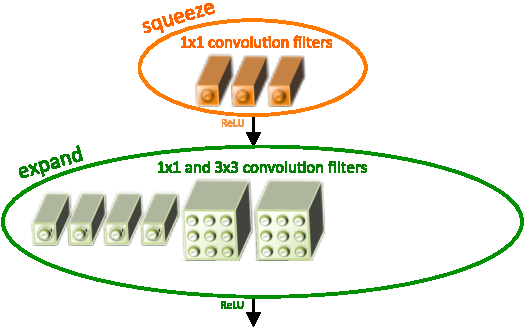
\includegraphics[width=\textwidth, height=0.3\textheight, keepaspectratio]{squeeze.pdf}
        \caption{Squeezenet Fire Module\cite{iandola_squeezenet_2016}}
        \label{fig:archi_building_block:sqn}
    \end{subfigure}
    %
    \begin{subfigure}[t]{0.49\linewidth}
        \centering
        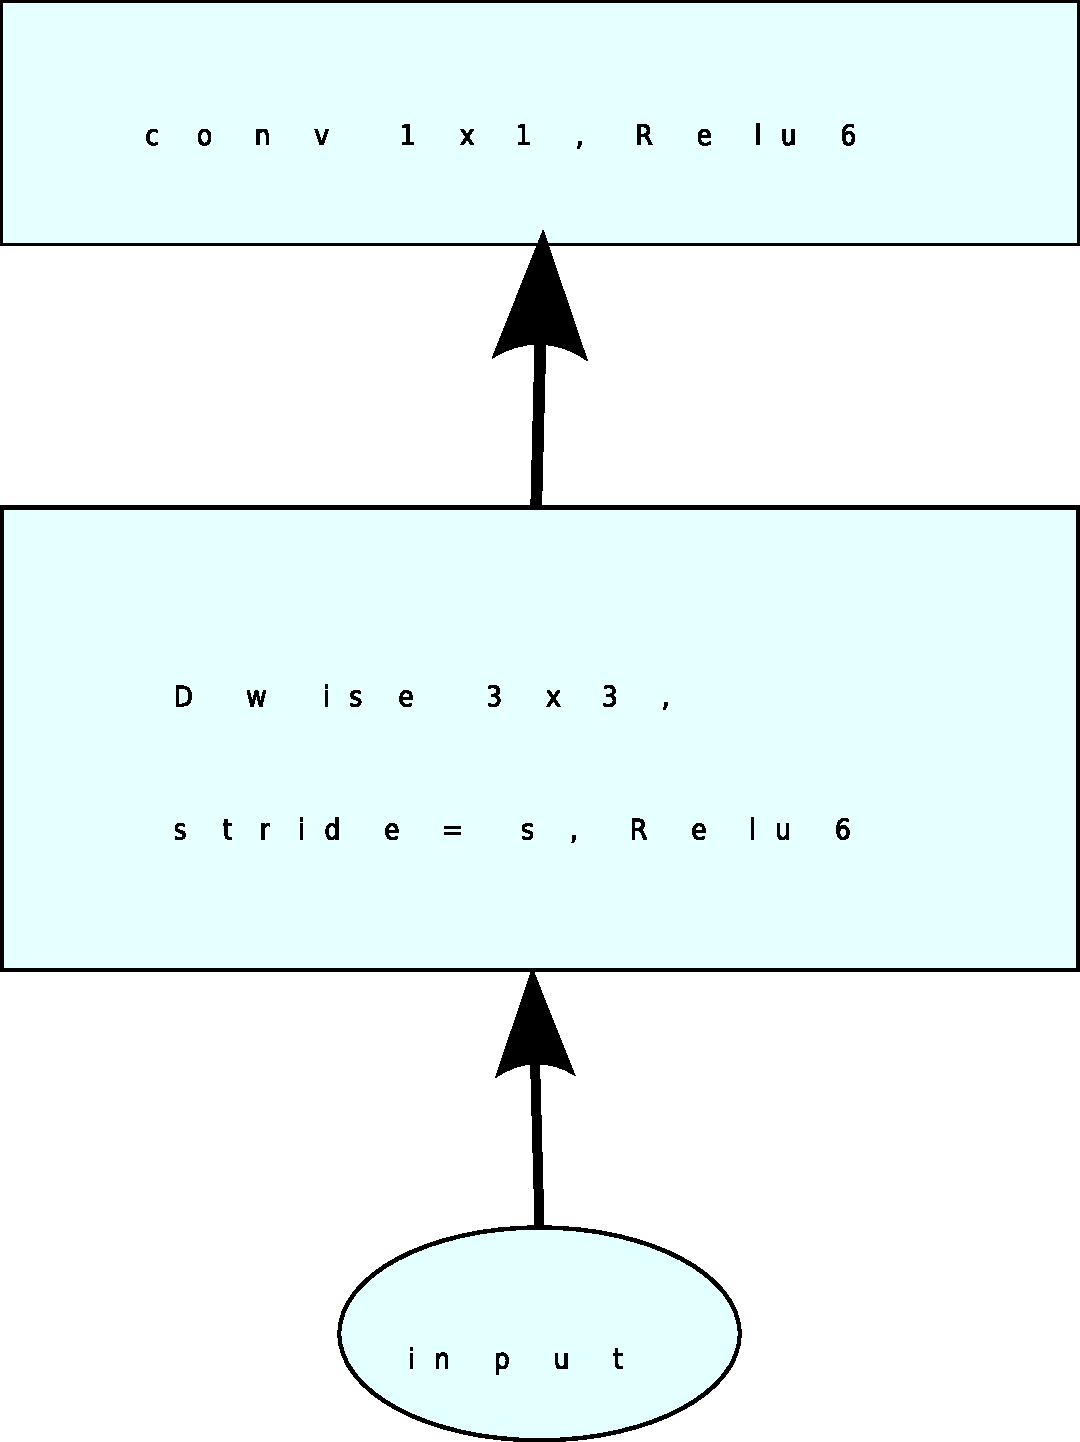
\includegraphics[width=\textwidth, height=0.2\textheight, keepaspectratio]{mobilenet.pdf}
        \caption{MobileNet convolutional block \cite{howard_mobilenets_2017}}
        \label{fig:archi_building_block:mbn}
    \end{subfigure}
    %
    \begin{subfigure}[t]{0.49\linewidth}
        \centering
        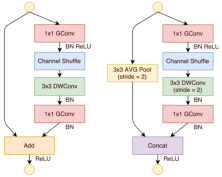
\includegraphics[width=\textwidth, height=0.2\textheight, keepaspectratio]{shufflenet.pdf}
        \caption{ShuffleNet convolutional block \cite{zhang_shufflenet_2018}}
        \label{fig:archi_building_block:shn}
    \end{subfigure}
    %
    \begin{subfigure}[t]{0.49\linewidth}
        \centering
        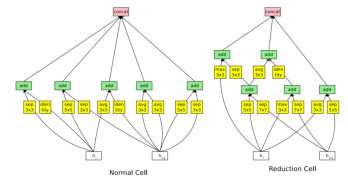
\includegraphics[width=\textwidth, height=0.3\textheight, keepaspectratio]{nasnet.pdf}
        \caption{NasNet convolutional blocks \cite{zoph_learning_2018}}
        \label{fig:archi_building_block:nasn}
    \end{subfigure}
    %
    \begin{subfigure}[t]{0.49\linewidth}
        \centering
        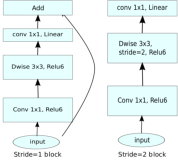
\includegraphics[width=\textwidth, height=0.2\textheight, keepaspectratio]{mobilenet2.pdf}
        \caption{MobileNetv2 convolutional blocks \cite{sandler_mobilenetv2_2018}}
        \label{fig:archi_building_block:mb2n}
    \end{subfigure}
    %
    \caption{Convolutional block from different architectures}
    \label{fig:archi_building_block}
\end{figure}

The architecture used in this work was developed to implement MobileNetV2 because of its simplicity and its state-of-the-art performance (see Table \ref{tab:mbv2}). Moreover, MobileNetV2 requires fewer parameters while providing state-of-the-art accuracy when comparing to the different architectures, as shown in Figure \ref{fig:archi}.
%
\begin{table}[H]
    \center
    \begin{tabular}{ | c | c | c c | c| }
        \hline \hline
        Network & Top 1 & Params & MAdds & CPU \\
        \hline \hline
        MobileNetV1 & 70.6 & 4.2M & 575M & 113ms \\
        ShuffleNet (1.5) & 71.5 & \textbf{3.4M} & 292M & - \\
        ShuffleNet (x2)  & 73.7 & 5.4M & 524M & - \\
        NasNet-A & 74.0 & 5.3M & 564M & 183ms \\
        \hline
        MobileNetV2 & \textbf{72.0} & \textbf{3.4M} & \textbf{300M} & \textbf{75ms} \\
        MobileNetV2 (1.4) & \textbf{74.7} & 6.9M & 585M & \textbf{143ms} \\
        \hline \hline
    \end{tabular}
    \caption{Performance on ImageNet, comparison for different networks \cite{sandler_mobilenetv2_2018}}
    \label{tab:mbv2}
\end{table}

\begin{figure}[H]
    \centering
    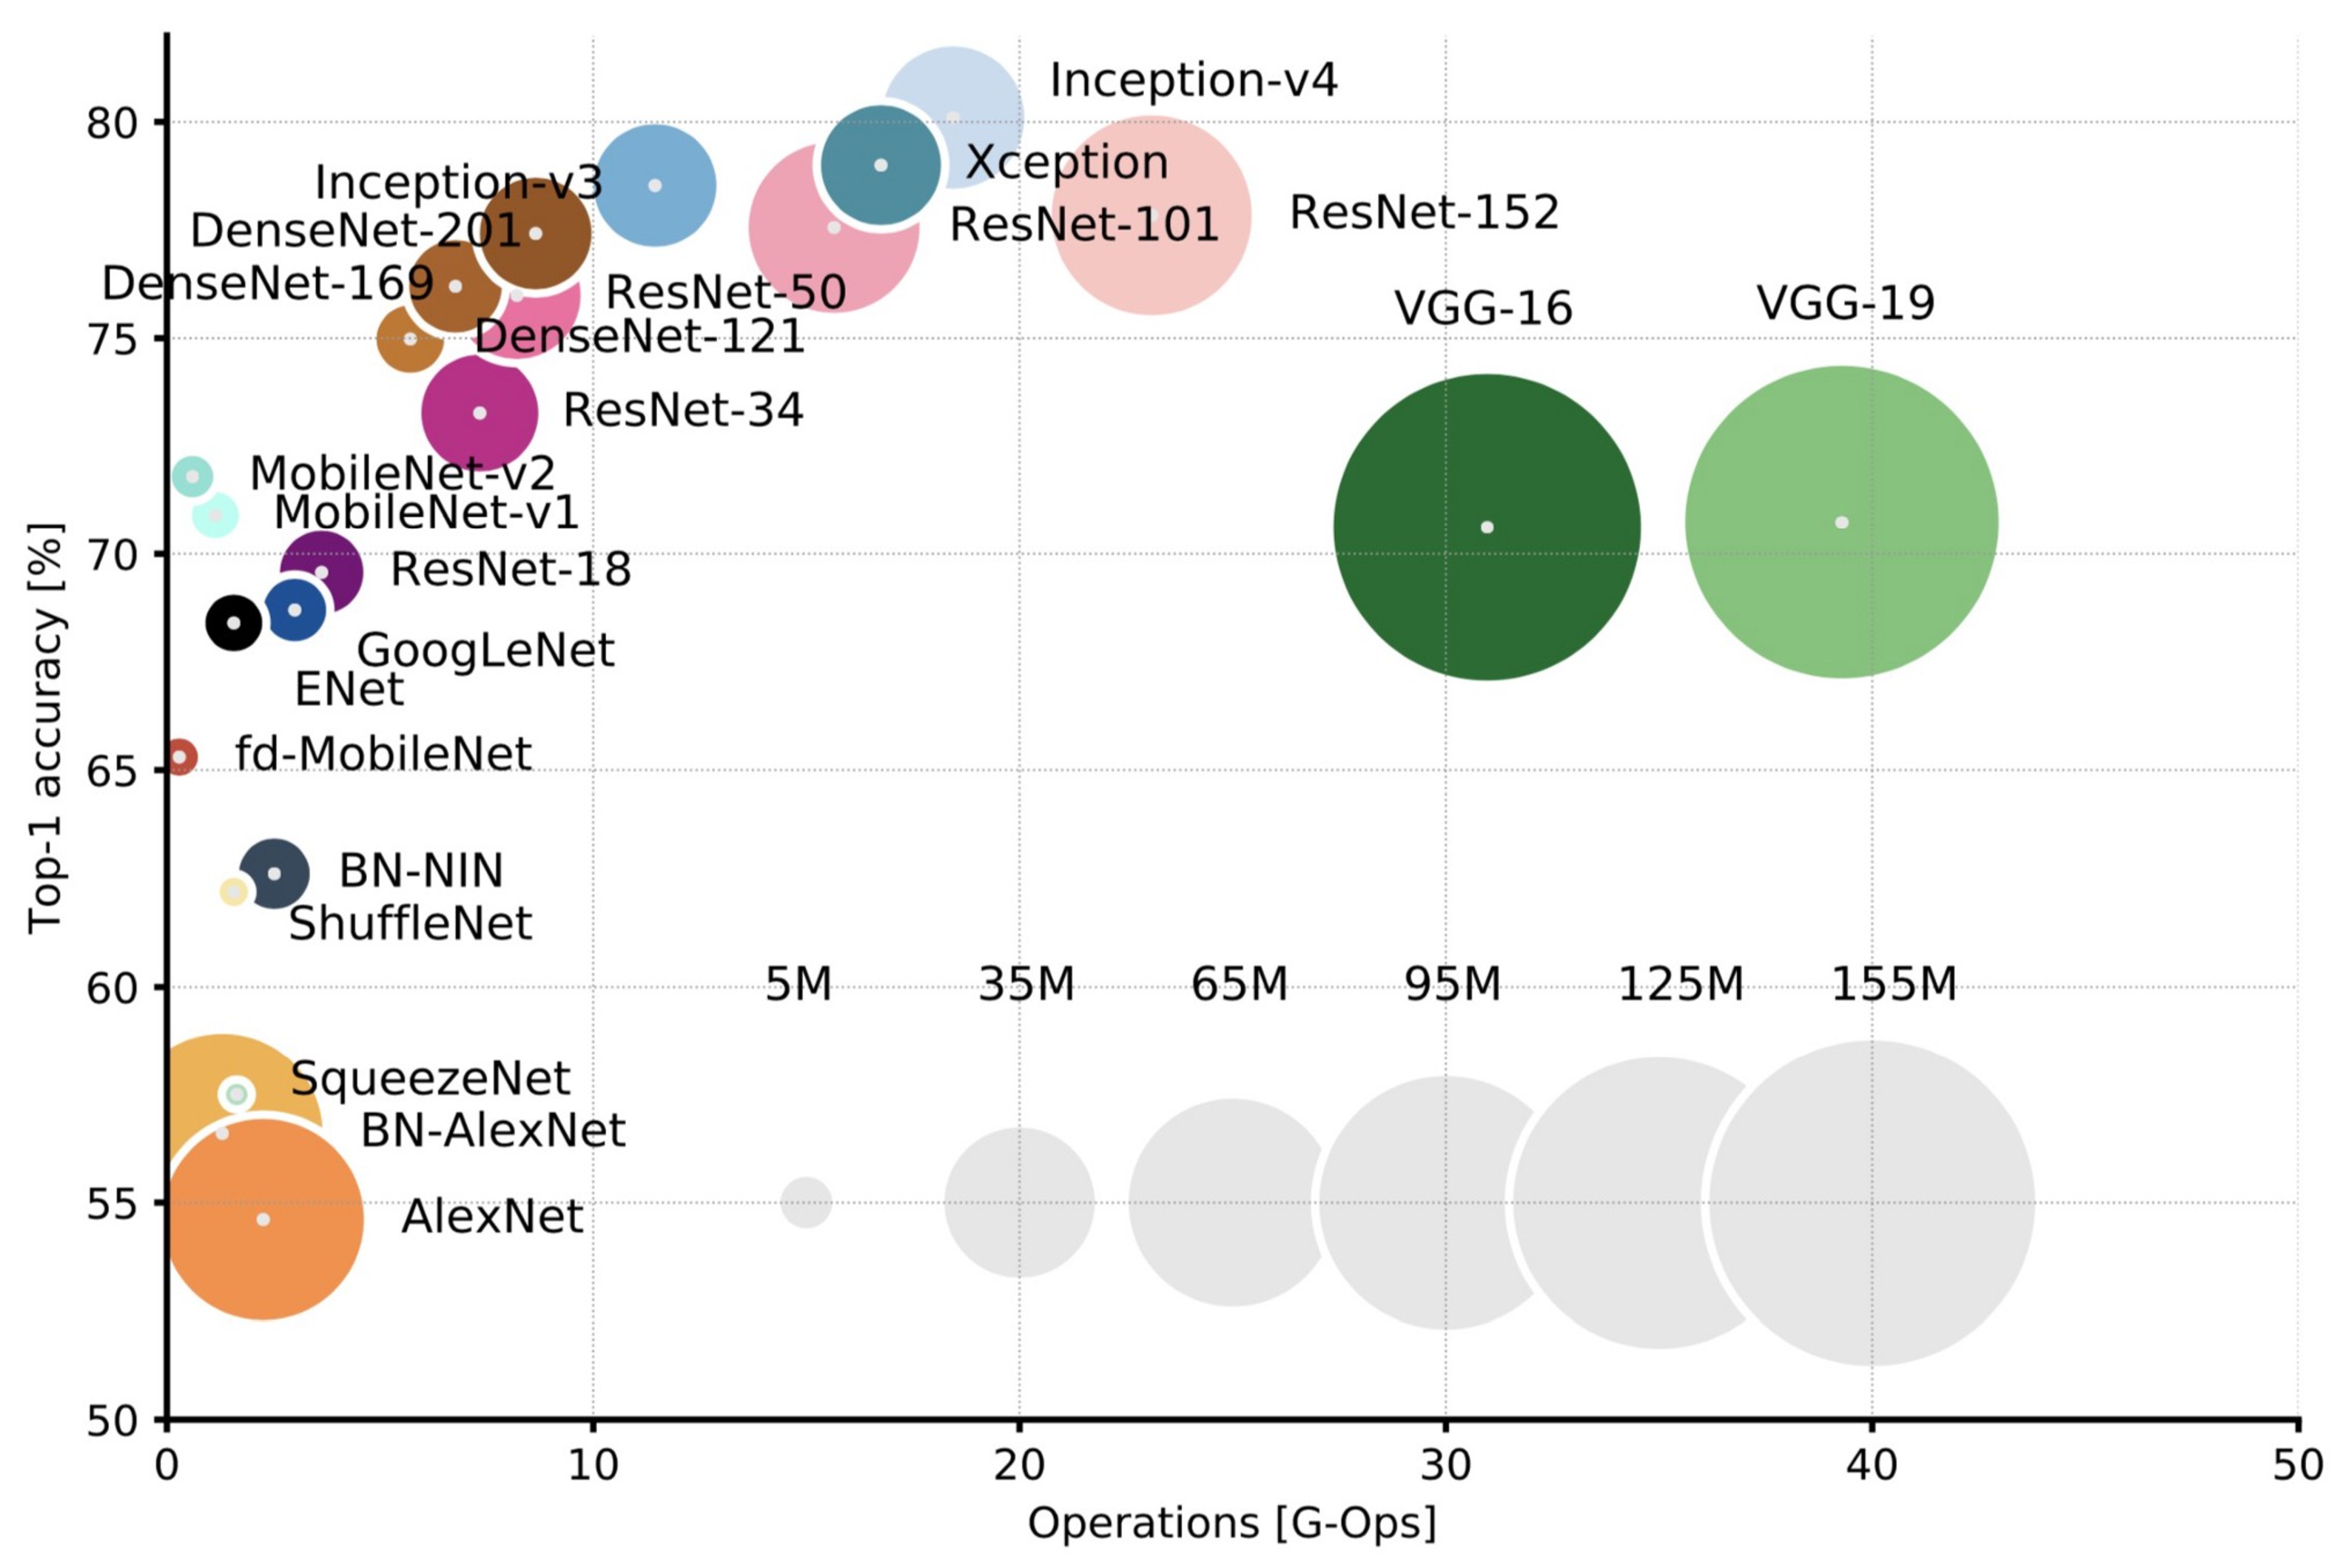
\includegraphics[width=0.9\textwidth]{archi.pdf}
    \caption{Ball chart reporting the Top-1 accuracy of various architectures vs. their computational complexity \cite{canziani_analysis_2017}}
    \label{fig:archi}
\end{figure}
%
\subsubsection{Pruning} \label{subs:pruning}
%
To improve the inference phase of a \acrshort{cnn}, pruning can be used, especially for platforms with limited computational resources \cite{liu_rethinking_2019}. According to \textcite{liu_rethinking_2019, denton_exploiting_2014}, the huge number of parameters in a network might create a problem of \textbf{over-parametrization}. Over-parametrization means that there are redundancies in \acrshort{nn} parameters and that the same performance could be achieved with only a subset of them. In other words, a lot of parameters are unimportant or unnecessary \cite{cheng_recent_2018}. Pruning is defined as removing the parameters considered as not important. For example, \textcite{baoyuan_liu_sparse_2015} achieve more than 90\% sparsity of parameters in convolutional layers in AlexNet with less than 1\% accuracy loss.

We can explain why pruning works by \textbf{The Lottery Ticket Hypothesis} \cite{frankle_lottery_2018, frankle_early_2020}: \textquote{\textit{A randomly initialized, dense neural network contains a subnetwork that is initialized such that—when trained in isolation—it can match the test accuracy of the original network after training for at most the same number of iterations.}} From this postulate, those unimportant weights can be set to zero (prune) because they do not improve the accuracy of the model.

According to \textcite{cheng_recent_2018}, pruning has two major benefits for the inference phase. First, less storage is required. Indeed, the non-pruned weights are sparsely distributed among the kernels. Thus, they can be stored in a compressed format reducing memory utilization. Second, pruning reduces the arithmetic complexity of the network. As convolutions perform a weighted sum with the input \acrshort{fm}, each \acrfull{mac} operation with a pruned weight can be discarded. Moreover, \textcite{han_learning_2015, mao_exploring_2017, kang_accelerator-aware_2020} pointed out that some pruning ratios can also improve the accuracy of the network, which can be explained by a form of regularization.

Various pruning schemes are focused on increasing the sparsity of the network without a drop of accuracy \cite{han_deep_2016, han_learning_2015}.  We call this pruning scheme where all unimportant parameters are pruned without extra constraint \textbf{unstructured pruning} \cite{cheng_recent_2018}. However, it is challenging to exploit the performance and the high parallelism of \acrshort{fpga} with this kind of pruned network. Indeed, this kind of pruning scheme creates irregularities in the data access pattern \cite{zhu_efficient_2020}. It means that the number of pruned weights is different in each kernel, and we should adapt the circuitry to the worst case. As a consequence, all filters conduct wasteful operations except the worst case \cite{shimoda_filter-wise_2019}. Furthermore, \textcite{anwar_structured_2017} pointed out that unstructured pruning requires overhead for computing addresses of the sparse non-pruned elements. Therefore, we should find pruning patterns that would be more hardware-friendly.

In contrast to the unstructured pruning, we have \textbf{structured pruning} schemes \cite{kang_accelerator-aware_2020}. They combine a structure regularization for accuracy and locality optimization for computation efficiency. According to \textcite{anwar_structured_2017}, \textquote{\textit{Structured pruning has no or little extra costs}}. We can categorize the various schemes into different groups \cite{cheng_recent_2018, kang_accelerator-aware_2020, anwar_structured_2017, wen_learning_2016}:
\begin{itemize}
    \item \textbf{Depth-wise}: all the weights of a layer are pruned. The layer is then removed.
    \item \textbf{Kernel-wise}: instead of pruning all the weights, we keep a ratio of kernels, which means a reduction of the number of output channels. This pruning scheme is provided in Figure \ref{fig:struct_pruning:fw}.
    \item \textbf{Channel-wise}: it is one of the most popular methods because it still can fit in the convolutional deep learning frameworks \cite{liu_rethinking_2019}. A layer of the input \acrshort{fm} is pruned, which means that the layer is also pruned in all the kernels, as can be seen in Figure \ref{fig:struct_pruning:chw}.
    \item \textbf{Shape-wise}: we prune the same weights in each kernel or group of kernels. For example, this pruning scheme was used in \textcite{zhu_efficient_2020}. It is illustrated in Figure \ref{fig:struct_pruning:sw}
\end{itemize}
%
\begin{figure}[H]
    \centering
    %
    \begin{subfigure}[t]{.32\textwidth}
    \centering
    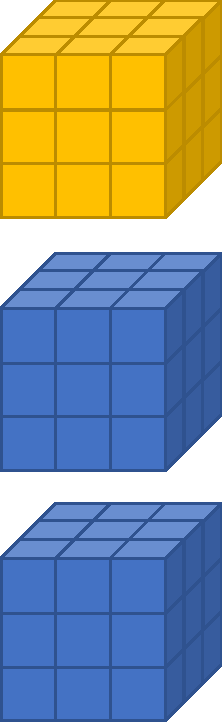
\includegraphics[width=0.33\linewidth]{filterwise.pdf}
    \caption{kernel-wise pruning}
    \label{fig:struct_pruning:fw}
    \end{subfigure}
    %
    \begin{subfigure}[t]{.32\textwidth}
    \centering
    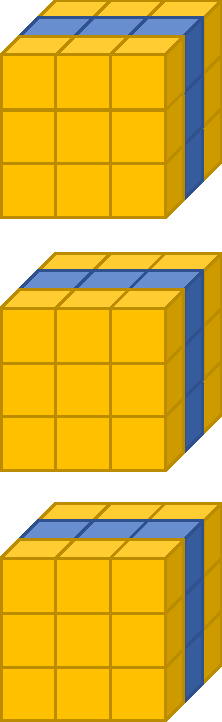
\includegraphics[width=0.33\linewidth]{channelwise.pdf}
    \caption{channel-wise pruning}
    \label{fig:struct_pruning:chw}
    \end{subfigure}
    %
    \begin{subfigure}[t]{.32\textwidth}
    \centering
    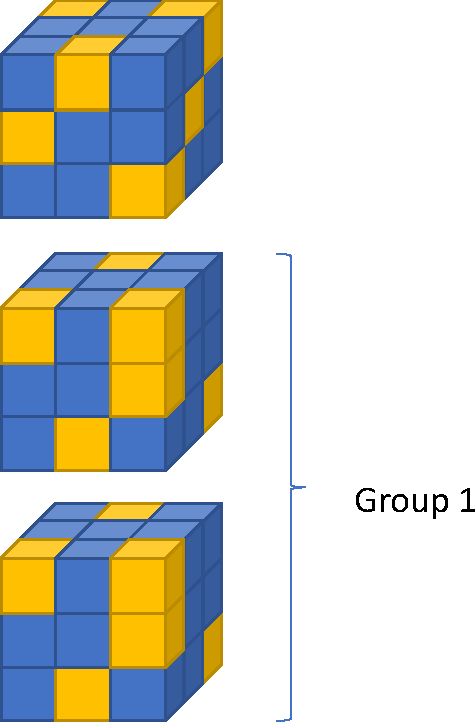
\includegraphics[width=0.70\linewidth]{shapewise.pdf}
    \caption{shape-wise pruning}
    \label{fig:struct_pruning:sw}
    \end{subfigure}
    %
    \caption{Structured pruning schemes, where the yellow weights are the pruned ones, inspired by \cite{cheng_recent_2018}}
    \label{fig:struct_pruning}
\end{figure}
%
The previously cited pruning schemes are ordered from very coarse-grained to fine-grained sparsity \cite{mao_exploring_2017}. As explained previously, coarse-grained sparsity (channel-wise and filter-wise pruning) provides a higher acceleration and can be used when implementing \acrshort{cnn} on \acrshort{gpu} or \acrshort{cpu} \cite{cheng_recent_2018, mao_exploring_2017}. However, finer-grained ones provide higher accuracy and as the sparsity increases, the accuracy is less affected, as can be seen in Figure \ref{fig:pruning-accuracy}. Therefore, this work focuses on developing customized hardware that can exploit a more fine-grained sparsity \cite{mao_exploring_2017} to provide a higher pruning while limiting the drop of accuracy.
%
\begin{figure}[H]
    \centering
    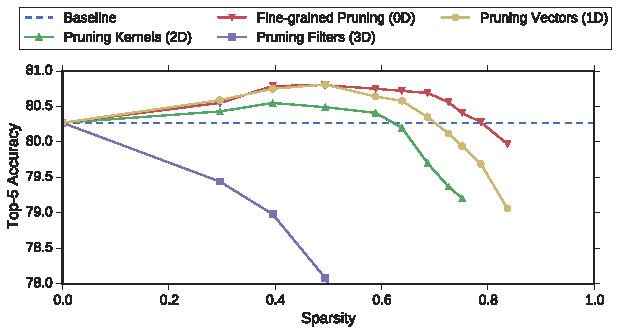
\includegraphics[width=\textwidth]{accuracysparsity.pdf}
    \caption{Accuracy-Sparsity Curve of AlexNet obtained by pruning \cite{mao_exploring_2017}}
    \label{fig:pruning-accuracy}
\end{figure}
%
Some studies focused on the acceleration of the inference step of lightweight models thanks to pruning. \textcite{zhang_channel_2019, tu_pruning_2019} applied pruning on \acrshort{dsc} kernels. They both chose \textbf{Channel-wise} pruning because it does not create sparse connections and it efficiently improves the speed of the inference. It also reduces the computational cost of the $1 \times 1$ (pointwise) convolutions, which has the biggest number of parameters and computational complexity. In MobileNet, it is about 95\%. By discarding one channel, the associated depthwise convolution is also avoided.
Moreover, the pointwise kernel producing that channel in the previous block can also be pruned. We can see the process in Figure \ref{fig:pruning_dsc}.
%
\begin{figure}[H]
    \centering
    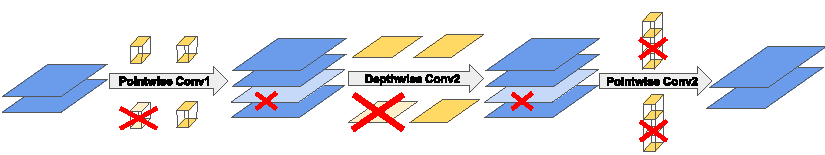
\includegraphics[width=\textwidth]{channelwise_ex.pdf}
    \caption{Pruning a depthwise separable convolution \cite{tu_pruning_2019}}
    \label{fig:pruning_dsc}
\end{figure}

\textbf{In this work, we focus on a structured pruning scheme for depthwise separable convolution. More precisely, we develop an architecture on \acrshort{fpga} than combines both advantages of pruning and depthwise separable convolution.}
%
\subsubsection{Quantization} \label{subs:quantization}
%
%
Quantization is an approach to trade accuracy for a decrease of the storage requirements of a network \cite{han_deep_2016}. Indeed, we can define quantization as the reduction of the number of bits representing a weight or pixel. Moreover, instead of using a floating-point number, we can use a \textbf{fixed-point number} \cite{cheng_recent_2018}. As said previously, fixed-point numbers are known to be more efficient on hardware such as \acrshort{fpga} because we can use integer arithmetic \cite{david_hardware_2007}. Quantization to fixed-point numbers can then reduce the memory requirement and the latency of the inference stage.

The format to encode the fixed-point representation of a real number is the \textit{Q-format} \cite{ward_real-time_2001}. A N-bit number, noted $Q_{m.n}$, is divided into two parts separated by an implied binary point. The $m$ bits are used to represent the integer part of the number (including the sign bit), and the $n$ bits are used to represent the fractional part, as can be seen in Figure \ref{fig:Qformat}. The bitwidth associated with each part can be either the same, either fine-tuned for each layer after analysis. Indeed, \textcite{qiu_going_2016, yin_high_2018} choose a different range for each layer, but doing it for every weight is not memory-efficient.
%
\begin{figure}[H]
    \centering
    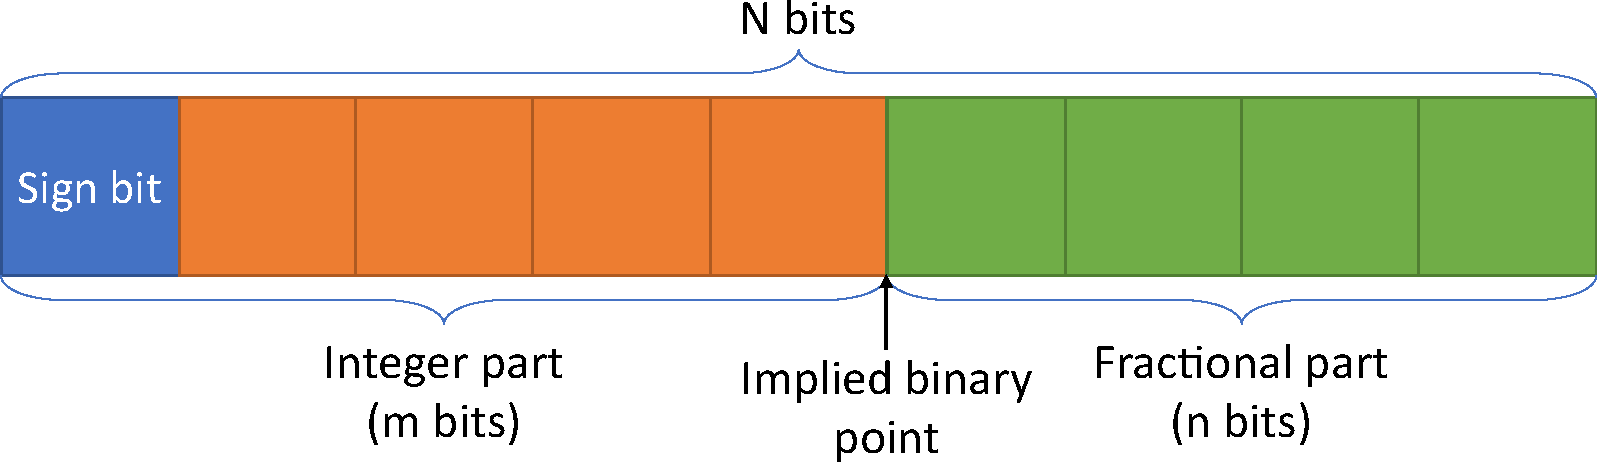
\includegraphics[width=\textwidth]{Qformat.pdf}
    \caption{Illustration of the Q-format}
    \label{fig:Qformat}
\end{figure}

As pointed out by \textcite{han_deep_2016}, quantization and pruning techniques are orthogonal and can be combined to compress further the network. Unfortunately, not all existing networks are friendly for quantization, like MobileNet. MobiletNet with quantized pixels and weights has a large drop of accuracy compared with its Non-quantized version (70.50\% using floating-point model vs 1.80\% using an 8-bit pipeline) \cite{sheng_quantization-friendly_2018}. However, the work of \textcite{sheng_quantization-friendly_2018} showed that the source of the accuracy drop was the design of the separable convolution core layer. They proposed therefore a new quantization-friendly separable convolution core layer. Works on MobileNetV2 should then be done to verify the fixed-point inference accuracy. Still, an 8-bit pipeline might not be optimal for MobilNetV2 as increasing the bitwidth to 16-bit could boost accuracy \cite{cheng_recent_2018}. This bitwidth is also widely used \cite{huimin_li_high_2016, bai_cnn_2018}. 

\textbf{Therefore, 16-bit fixed-point Q-format is adopted for input data, weights, and intermediate data in the frame of this thesis}. \textbf{Moreover, as said previously in Section \ref{subs:acti}, we can limit the integer part to 3 bits (one bit is added to express the sign of the weights), and we can use $Q_{4.12}$.}


%
\chapter{Accelerating \acrshort{cnn} inference on \acrshort{fpga}}
\label{chap:inf}
As said at chapter \ref{chap:intr}, interest has been made on accelerating the inference phase on \acrshort{fpga}. This chapter reviews the acceleration approaches to perform an efficient inference. \newline \newline
The three main optimization can be categorized according to \cite{abdelouahab_accelerating_2018}:
\begin{itemize}
    \item \textbf{Algorithmic Optimizations}: the computational cost of the convolution can be reduced by vectorizing them. More details can be found in section \ref{sec:algopti}.
    \item \textbf{Datapath Optimization}: because of the limited resources on a \acrshort{fpga}, memory if often the bottleneck and optimizing the memory management can increase the throughput. More details can be found in section \ref{sec:dtptopti}.
    \item \textbf{\acrshort{cnn} model Optimization}: an important issue of \acrshort{cnn} is their computational complexity and their hardware utilization. A solution is then to use approximate computing and trade accury for acceleration. This work focus on this kind of optimization. More details can be found in section \ref{sec:mdopti}.
\end{itemize}
%%%%%%%%%%%%
\section{Algorithmic Optimizations} \label{sec:algopti}
In this section we will review algorithmic optimization techniques to reduce computational complexity of convolutions, which are a costly operation. According to \cite{shawahna_fpga-based_2019}, 90\% of computation time in \acrshort{cnn} are consummed by the convolution operation.
%
%
\subsection{\acrfull{gemm}}
%
%
It is a common way to process \acrshort{cnn} on \acrshort{cpu} and \acrshort{gpu}. We convert the convolution as a matrix-vector multiplication.  The process of a convolution layer can be observed on Figure \ref{fig:gemm}.
However, this approach is not suggested for \acrshort{fpga}: \cite{sze_efficient_2017, zhu_efficient_2020} point out that the \acrshort{fm}s have to be copied multiple times when flattened to a vector. It leads to a huge memory footprint and either ineffiency in storage or complex memory management access patterns.
\begin{figure}
    \centering
    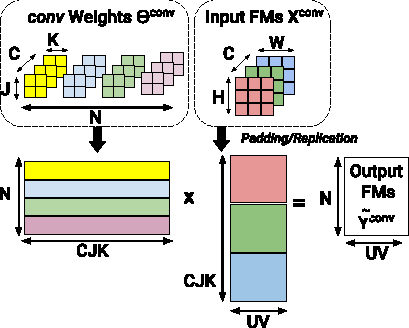
\includegraphics[width=0.5\textwidth]{Images/gemm.pdf}
    \caption{\acrshort{gemm} base processing on conv layer}
    \label{fig:gemm}
\end{figure}
%
%
\subsection{Winograd Transform}
%
%
The Winograd minimal filter algorithm is first introduced by \cite{winograd_arithmetic_1980}. We can apply this computational transform to convolutions when the stride is equal to 1. In Winograd filtering, data is processed by blocs referred as \textit{tiles}, as following:
\begin{itemize}
    \item An input \acrshort{fm} tile $g$ of size $(N_{ix} \times N_{iy})$ is pre-processed: $\tilde{g} = \boldsymbol{G^{T}} g \boldsymbol{G} $, where $\boldsymbol{G}$ is a transformation matrix defined in the Winograd Algorithm \cite{winograd_arithmetic_1980}.
    \item In a same way, $d$, the filter of size $(K_x \times K_y)$ is transformed into $\tilde{d}$: $\tilde{d} = \boldsymbol{B^{T}} d \boldsymbol{B}$ , where $\boldsymbol{B}$ is a transformation matrix defined in the Winograd Algorithm \cite{winograd_arithmetic_1980}.
    \item The output tile $Y$ of the Winograd Filtering algorithm, denoted $F(N_{ix} \times N_{iy}, K_x \times K_y)$ is computed using equation \ref{eqn:winograd}, where $\boldsymbol{A}$ is a transformation matrix defined in the Winograd Algorithm \cite{winograd_arithmetic_1980} and $\odot$ indicates element-wise multiplication.
\end{itemize}
\begin{equation}
\label{eqn:winograd}
Y = \boldsymbol{A^{T}} [ \ \tilde{g} \odot \tilde{d} \ ] \boldsymbol{A}
\end{equation}
\cite{lavin_fast_2015} demonstrated that Winograd convolution is efficient when the kernel is small ($K_* \leq 3$) and the number of multiplication can be reduced by a factor of $2.25 \times$ (in returns the number of addition is increased). According to \cite{sandler_mobilenetv2_2019}, $3 \times 3$ kernel is a standard for modern networks, which leads to think that Winograd Transform is a usefull approach to reduce computational complexity of convolutional layers. For example, \cite{aydonat_opencl_2017, lu_evaluating_2017} utilized Winograd transform and haved reduced their computational complexity by around 50\%.
%
%
\subsection{\acrfull{fft}}
%
%
The \acrshort{fft} is an algorithm to transform the 2D convolution into element-wise multiplication in the frequency domain. The equation is observed at equation \ref{eqn:fft}
\begin{equation}
\label{eqn:fft}
conv2D(FM_{I}[ic], K[oc, ic]) = IFFT( FFT(FM_{I}[ic]) \odot FFT(K[oc, ic]) )
\end{equation}
The arithmetic complexity of the 2D convolution can be reduced to $O(N_{ix}^2 log_2(N_{ix}))$ \cite{jong_hwan_ko_design_2017} and the computational complexity of the \acrshort{fft} can be reduced to $O(N_{ix} log_2(K_{x}))$ using the Overlap-and-Add Method \cite{w_smith_scientist_1997}.
However, the \acrshort{fft} finds its interest when kernel are large \cite{lavin_fast_2015} ($K_* \geq 5$), which is not a standard kernel size according to \cite{sandler_mobilenetv2_2019}. \cite{zhang_frequency_2017} implemented \acrshort{fft} algorithm for \acrshort{cnn} on \acrshort{fpga} and it showed little reduction of computation complexity with small filters such as $3 \times 3$.

%%%%%%%%%%%%
\subsection{General CNN inference on FPGA} \label{sec:dt_general}
%
As described in Section \ref{sec:fpga}, \acrshort{fpga} is an array of programmable gates that can interface with the outside world. As a result, to perform the convolution operation, the \acrshort{fpga} has to fetch weights and input \acrshort{fm} from the outside world (for example an external memory) and compute the convolution with them. Once the result is obtained, the \acrshort{fpga} can output the results through its \acrshort{ioe}.

According to \textcite{chen_eyeriss_2017}, the data movement can often be more energy-consuming than actual computation. Therefore, smart memory management is required to implement \acrshort{cnn} on low power devices such as \acrshort{fpga}. We discover in this section various techniques for handling the Datapath on the \acrshort{fpga}.

\subsubsection{Systolic Arrays}
%
%
Systolic arrays were implemented on the early \acrshort{fpga}-based accelerators \cite{abdelouahab_accelerating_2018, farabet_cnp_2009, gokhale_240_2014}. A static systolic array is a static array of \acrfull{pe}, controlled by the \acrshort{cpu}. The \acrshort{pe} is the basic computing unit for convolution. Therefore, each \acrshort{pe} is involved in a part of the computation and can communicate with adjacent \acrshort{pe}s. An illustration of this principle can be found in Figure \ref{fig:sytar}. The configuration can only support convolution with a kernel size $K_*$ lower than a maximal kernel size, such that $K_* \leq K_m$ (because the number of \acrshort{pe} is fixed). The systolic array allows spatial data reuse between rows and columns, high clock frequency, and temporal data reuse using \acrshort{fifo} queues \cite{joos_de_ter_beerst_accelerating_2019, mittal_survey_2020}.
%
\begin{figure}[H]
    \centering
    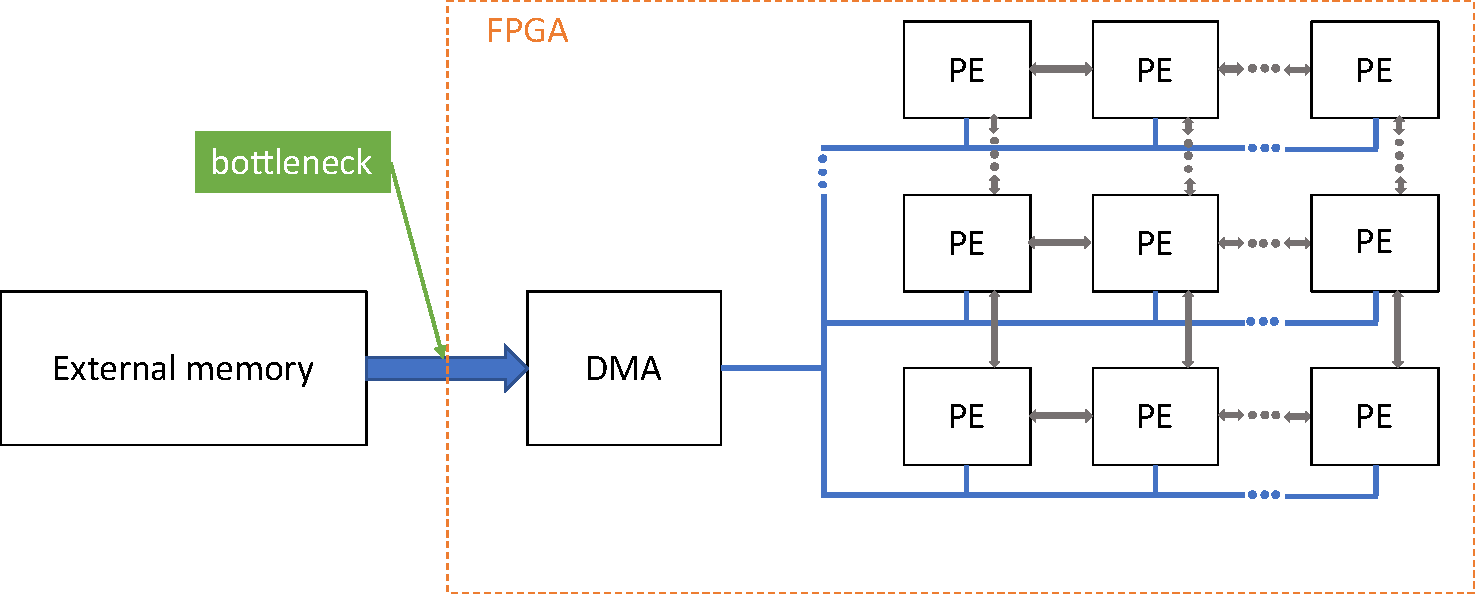
\includegraphics[width=\textwidth]{systArray.pdf}
    \caption{Static Systolic Arrays, inspired by \cite{abdelouahab_accelerating_2018}}
    \label{fig:sytar}
\end{figure}

However, Systolic Arrays have inefficiency problems. First, when the kernel size is much smaller than the maximal kernel size ($K_* << K_m$), there is an underutilization of the resources. For example, \cite{gokhale_240_2014} notes that for $3 \times 3$ kernels, only $9\%$ of the \acrfull{dsp} blocks are used. Second, data caching is not implemented. It means that it has always to fetch input from the external memory and it increases latency \cite{abdelouahab_accelerating_2018, wei_automated_2017}. The device performance is depending then on the memory bandwidth and it becomes memory-bounded. Furthermore, it is not energy efficient. According to \textcite{horowitz_11_2014}, the DRAM accesses severely impact both throughput and energy efficiency. External memory accesses are more expensive by several orders of magnitude in terms of energy and latency.
%
%
\subsubsection{Data-flow MoC for CNNs (2D mapping)}
%
%
Data-flow \acrfull{moc} can be used to accelerate \acrshort{cnn}s on \acrshort{fpga}. This approach is motivated by the feed-forward aspect of the inference stage of \acrshort{cnn}, which is purely data-driven \cite{abdelouahab_accelerating_2018}. Data-flow \acrfull{moc} was firstly investigated by \textcite{lin_li_low_2016}. \acrshort{cnn} can be represented as a graph where:
\begin{itemize}
    \item \textbf{Nodes} are processing units called \textit{actors}. Each actor follows a data-driven execution where the execution is triggered by the availability of input, which is the case for a \acrshort{cnn}.
    \item \textbf{Edges} are communication \acrshort{fifo} channels. Actors exchange data called \textit{tokens} through those \acrshort{fifo} channels.
\end{itemize}
A representation of such a network can be found in Figure \ref{fig:moc}, where $FM_{*}^{i}$ is the ith layer of the \acrshort{fm}.
%
\begin{figure}[H]
    \centering
    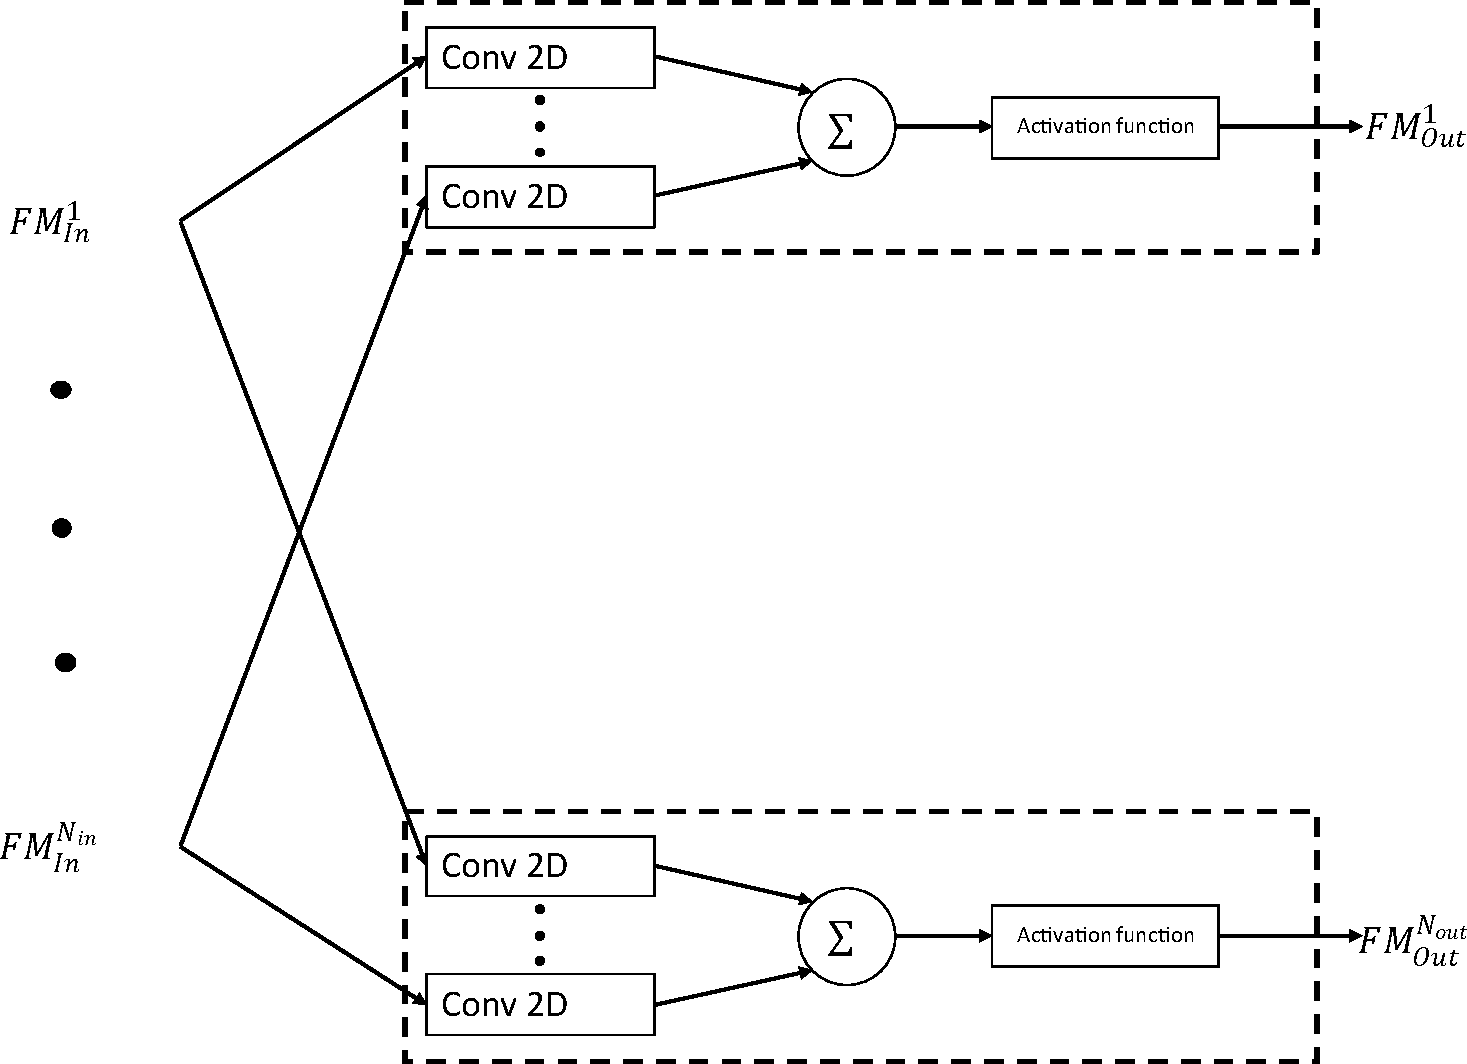
\includegraphics[width=0.6\textwidth]{Moc.pdf}
    \caption{Graph representation of a convolution layer, inspired by \cite{abdelouahab_accelerating_2018}}
    \label{fig:moc}
\end{figure}

As the number of tokens produced and consumed by an actor can be specified in a \acrshort{cnn}, we can apply a static data-flow \cite{lee_static_1987}. Therefore the \acrshort{cnn} can be modeled as a topology matrix and we only need to optimize those matrix components to minimize latency or energy consumption \cite{venieris_latency-driven_2017}. Those parameters are then used to derive \acrshort{pe} and buffer configurations. However, as pointed by \textcite{abdelouahab_tactics_2017}, we need to have direct hardware mapping between the graph and the \acrshort{fpga} to be efficient. It means that all the computations must be unrolled. However, we are then bounded by the hardware resources and the size of \acrshort{cnn}, preventing implementing this approach for deep models \cite{abdelouahab_accelerating_2018}.
%
\subsubsection{Loop Optimizations} \label{subsec:loopopti}
%
%
To overcome the inefficiencies of Systolic arrays and because Data-flow \acrshort{moc} can only be applied to small networks, data must first be cached into the on-chip memory of the \acrshort{fpga} before processing. However, according to \textcite{ma_optimizing_2018}, the on-chip memory of \acrshort{fpga} is not large enough to store all the data (requiring gigabytes). As a result, we need \textit{tiling} to fit a smaller portion of data into memory on-chip \cite{zhang_optimizing_2015}. We can summarize the dataflow as follow: the \acrshort{fpga} fetches a tile of data from external memory to on-chip buffers. Then the data is fed to the \acrshort{pe}s to compute the convolution. The results of the computation are transferred back to on-chip buffers and afterward, to the external memory. When the results are written back to memory, we can fetch a new tile of data. We can see the process in Figure \ref{fig:hierarchy}
%
\begin{figure}[H]
    \centering
    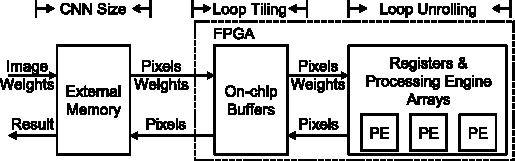
\includegraphics[width=0.75\textwidth]{memhiera.pdf}
    \caption{\acrshort{fpga} memory hierarchy, from \cite{ma_optimizing_2018}}
    \label{fig:hierarchy}
\end{figure}

Consequently, we can define a storage hierarchy with different energy costs. We can define the memory levels as \cite{sze_efficient_2017, horowitz_11_2014}:
%
\begin{enumerate}
    \item \textbf{External Memory}: it stores all the \acrshort{cnn} data. It has a large memory capacity (\textasciitilde GB) but accesses are costly in terms of energy and latency.
    \item \textbf{On-chip memory}: it stores the data fetched from external memory to feed the registers and \acrshort{pe}s. Accesses are less expensive to the external memory but it has less storage (\textasciitilde hundreds of KB).
    \item \textbf{Register}: is associated with the \acrshort{pe}s. The storage capacity is less than a few KB but it is faster and more energy-efficient. Accesses are 1 or 2 orders of magnitude lower energy than from External memory.
\end{enumerate}

Therefore, after tiling, the convolution operation can be decomposed in multiple loops, as observed in Figure \ref{fig:looptiling}. Nevertheless, an improper loop tiling may degrade the performance of the \acrshort{fpga} because we must minimize access to expensive memory levels. The major challenge when implementing a \acrshort{cnn} on \acrshort{fpga} is then to maximize data reuse in small cost memories. To address those problems, loop optimization techniques are applied to the nested loops in Figure \ref{fig:looptiling}. There are three techniques:
%
\begin{enumerate}
    \item \textbf{Loop tiling}: as said above, the on-chip memory of the \acrshort{fpga} is not large enough to store all the weights and \acrshort{fm}s of all \acrshort{cnn} layers \cite{abdelouahab_accelerating_2018}. The \acrshort{fpga} stores a tile of the data, accessed from the external memory, and the lower bound is set on the required on-chip buffer size. The tiling parameters represent the tile size. They are defined as $T_{*}$, where $*$ is the name of the dimension. For example, the size of an input pixel buffer (resp. output) is $T_{ix} \times T_{iy} \times T_{if} \times $ pixel\_datawith ( $ T_{ox} \times T_{oy} \times T_{of} \times $ pixel\_datawith). Furthermore, we have the following constraint: $T_{*} \leq N_{*}$.
    \item \textbf{Loop interchange}: it defines the order of sequential computation of the convolution loops. There are 2 types of loop interchange: \textit{intratile}, patterns of data movements from on-chip memory to registers (loop one to four in Figure \ref{fig:looptiling}); \textit{intertile}, patterns of data movements from external memory to on-chip buffers (the other loops).
    \item \textbf{Loop unrolling}: it determines the number of parallel computations. Four types of unrolling configuration can be done (depending on the loop to unroll). The different configurations can be seen in Figure \ref{fog:unroll}. As the \acrshort{fpga} has constrained resources, it is not always possible to fully unroll a loop. The unrolling parameters are defined as: $P_{*}$, where $*$ is the name of the dimension. We also have the following constraint: $P_{*} \leq T_{*} \leq N{*}$.
\end{enumerate}
%
\begin{figure}[H]
\centering
\begin{lstlisting}[language=Java]
for (int of=0;of<N;of+=Tof){
  for (int iy=0;iy<Niy,iy+=Tiy){
    for (int ix=0;ix<Nix,ix+=Tix){
      for (int if=0;n<C;if+=Tif){
        // DRAM: Load in on chip buffers the tiles
        // X[l,if:if+Tif,iy:iy+Ty,ix:ix+Tix]
        // Theta [l,n:n+Tof,if:if+Tif,j,k]
          for (int tof=0;tof<Tof;tof++){ -> Loop-4
            for (int tiy=0;tiy<Tiy,tiy++){ -> Loop-3
              for (int tix=0;tix<Tix,tix++){ -> Loop-3
                for (int tif=0;tof<Tif;tif++){ -> Loop-2
                  for (int ky=0;ky<Nky,ky++){ -> Loop-1
                    for (int kx=0;kx<Nkx,kx++){ -> Loop-1
                      Y[tof,tiy,tix] += X[tif,tiy+ky,tix+kx] *
                      W[tof,tif,ky,kx];
          }}}}}}
          // DRAM: Store output tile
}}}}
    \end{lstlisting}
    \caption{Loop Tiling, from \cite{abdelouahab_accelerating_2018}}
    \label{fig:looptiling}
\end{figure}
%
\begin{figure}[H]
    \centering
    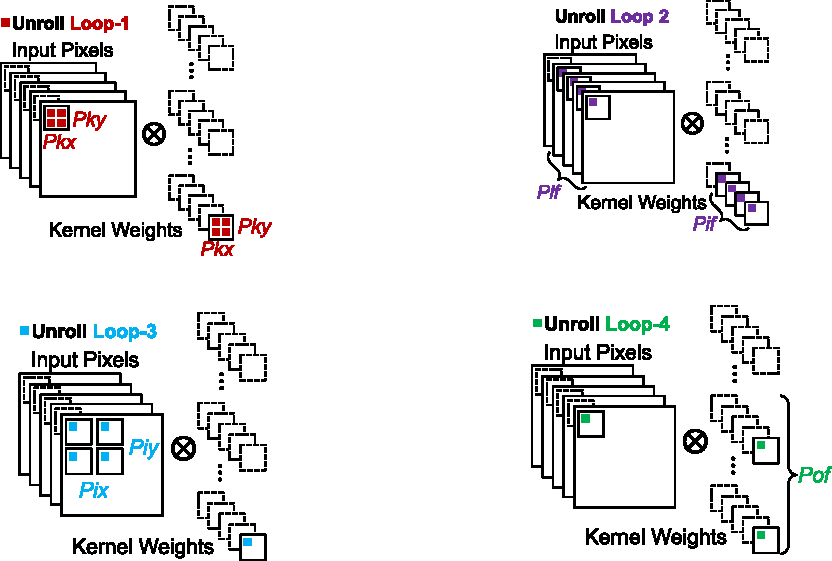
\includegraphics[width=\textwidth]{unroll.pdf}
    \caption{Loop unrolling configurations, from \cite{ma_optimizing_2018}}
    \label{fog:unroll}
\end{figure}

The loop optimization design variables determine the number of \acrshort{pe}s (unrolling parameters), the buffer size, and the number of external memory access (tiling parameters). We are going to review different studies of the design space exploration of unrolling parameters, tiling parameters, and loop interchange, to design the most efficient accelerator on the target platform.

The work of \textcite{zhang_optimizing_2015} proposes an analytical solution using the roofline model \cite{williams_roofline_2009} to identify the CNN design with the best performance and lowest \acrshort{fpga} resource requirement. They chose a loop unrolling of ($T_{if} \times T_{of}$) to avoid complex connection topologies for all arrays. It allows spatial reuse of pixels for $T_{of}$ unrolls, and the temporal reuse of weight for ($T_{ox} \times T_{oy}$). However, the disadvantage of this method is the need for a large local memory to store the partial sums ($T_{of} \times T_{ox} \times T_{oy}$).

Once the loop ordering and unrolling parameters have been set, the roofline model can be used to find the optimal tiling parameters. \textcite{mittal_survey_2020} defines this design space exploration method as: \textquote{\textit{The roofline model relates performance to computational performance and off-chip memory traffic}}. As an implementation can either be computation-bounded or memory-bounded, it uses those two limits to find the best trade-off between memory bandwidth and computational speed, where $CTC$ is the communication-to-communication ratio.
\begin{enumerate}
    \item \textbf{Computational roof}: $= \frac{\text{\# \ of \ operations}}{\# \ of \ execution \ cycles}$.
    \item \textbf{CTC ratio}: $= \frac{\text{\# \ of \ operations}}{\# \ of \ external \ data \ access}$
\end{enumerate}
Therefore, the achievable performance can be computed using equation \ref{eq:atperf}.
\begin{equation}
Att \ perf = min \ (Computational \ roof; CTC \ ratio \times bandwidth)
\label{eq:atperf}
\end{equation}

The roofline method is shown in Figure \ref{fig:roofmeth}. We can conclude that the best solution to pick is solution C since it offers the best performance while requiring the least bandwidth \cite{zhang_optimizing_2015}.
%
\begin{figure}[H]
    \centering
    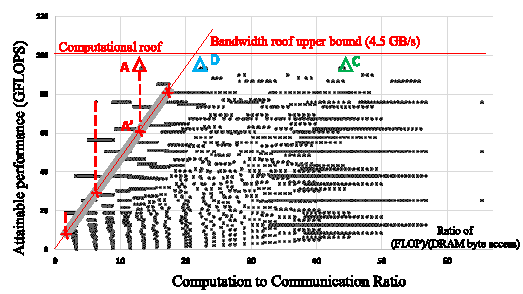
\includegraphics[width=\textwidth]{roofmethod.pdf}
    \caption{Design space of platform-supported designs, from \cite{zhang_optimizing_2015}}
    \label{fig:roofmeth}
\end{figure}

\textcite{motamedi_placid_2017} chose the best parameters according to the resources and the best data reuse scheme of the target platform. They did not tile on the kernel on the spatial axis because recent \acrshort{cnn}s have small filters and it would mean that a pixel can be loaded multiple times. As the tile goes over the input and output \acrshort{fm} channel, there is a choice between maximizing the reuse of the input \acrshort{fm} (MIR, each \acrshort{fm} is loaded once but some intermediate results have to be written back to memory) or output \acrshort{fm} (MOR, to avoid writing back intermediate results to memory but some input \acrshort{fm} have to be loaded more than once). Then they performed an exhaustive search on the tiling and \acrshort{pe} parameters to find the optimal design. It can be layer-specific (but the \acrshort{fpga} needs dynamic reconfiguration and \textcite{zhang_optimizing_2015} proved that it is inefficient) or values are fixed for all layers.

A different approach, studied by \textcite{ma_optimizing_2018}, proposes a design space exploration regarding various design objectives:
\begin{itemize}
    \item \textbf{Latency}: $P_*$ should be common factors of  $T_*$ for all convolution layers to fully utilize \acrshort{pe}s and $T_*$ should be the common factors of  $N_*$ to make full use of external memory transactions.
    \item \textbf{Partial sum storage}: to minimize the concurrent storage of partial sums in local memory and allowing to keep them into the PE, we should promote the computation of an output pixel to evacuate it to the external memory.
    \item \textbf{On-chip memory access}: on-chip memory access can be minimized by reusing at most pixels or weights in the \acrshort{pe}s.
    \item \textbf{External memory access}: to minimize external access, a sufficient buffer size should be assigned to pixels and weights.
\end{itemize}

They proposed two flowcharts in Figure \ref{fig:flowchart} to determine the number of partial sums and external accesses. 
%
\begin{figure}[H]
\centering
    \begin{subfigure}{.45\textwidth}
    \centering
    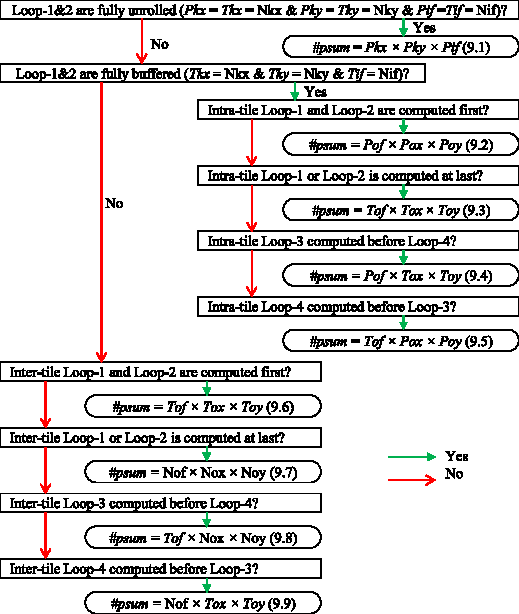
\includegraphics[width=\linewidth]{fwch1.pdf}
    \caption{ }
    \end{subfigure}
    \begin{subfigure}{.45\textwidth}
    \centering
    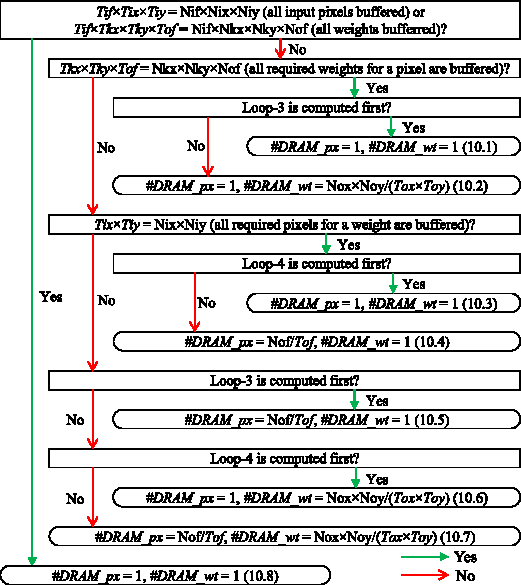
\includegraphics[width=\linewidth]{fwch2.pdf}
    \caption{ }
    \end{subfigure}
    \caption{Design space exploration of: (a) total number of partial sums that need to be stored in memory; (b) the number of external memory accesses, from \cite{ma_optimizing_2018}}
    \label{fig:flowchart}
\end{figure}

%%%%%%%%%%%%
\subsection{Model Optimizations} \label{subsec:mdopti}
As mentioned previously, the major issues, when implementing a \acrshort{cnn} on an \acrshort{fpga}, are the \acrshort{cnn} size and its computational complexity. Research was done to develop techniques tackling those two issues by directly modifying the \acrshort{cnn} architecture. \textcite{nurvitadhi_can_2017} believe that sparsity exploitation and extremely compact data types will become the norm in next-generation \acrshort{cnn}s.
%
%
\subsubsection{Efficient Model Design}
%
Section \ref{subsec:models} presented several state-of-the-art models. However, those models (except MobileNetV2) were designed to provide the highest performance possible but did not consider the implementation of such models on mobile and embedded devices \cite{iandola_squeezenet_2016}. Therefore, several other models were designed to run on such constrained platforms trading a reduction of the number of parameters and operations in exchange for a drop of accuracy. Indeed, if we observe Figure \ref{fig:archi}, the lightweight models do not match the high-performance ones in terms of accuracy only.

A clever choice of design decreases the number of parameters and computations of the model while reducing the drop of accuracy. As many approaches were proposed to reduce the size of a model, this study will focus on architectures that target the embedded space. This section describes five of these architectures:
\begin{itemize}
    \item \textbf{SqueezeNet} \cite{iandola_squeezenet_2016} was focused on reducing the number of parameters of AlexNet (see Section \ref{subsec:models}) by introducing a new building block: \textbf{Fire Module}. Therefore, their architectures are very similar. SqueezeNet replaces all layers (except the first and last one) by \textbf{Fire Modules}. The \textbf{Fire Module}, observed in Figure \ref{fig:archi_building_block:sqn}, is composed of two convolutional layers. The first one called \textit{squeeze block} only performs $1 \times 1$ convolutions to squeeze the number of input channels. The reduction of the number of channels decreases the computational complexity and number of parameters of the next convolutional layer. Moreover, they also chose $1 \times 1$ convolution because it requires fewer parameters than $3 \times 3$ convolution.
    The second convolutional layer called \textit{expand block} is composed of $1 \times 1$ and $3 \times 3$ convolutions. With this architecture, the size of AlexNet is decreased from $240$MB to $4.8$MB \cite{iandola_squeezenet_2016}. It can even be reduced to $0.47$MB without a drop in accuracy method by applying Deep Compression \cite{han_deep_2016}. However, it has a big memory footprint, is slower in runtime, and consumes more energy than AlexNet \cite{sze_efficient_2017}.
    %
    \item \textbf{MobileNet} \cite{howard_mobilenets_2017} uses \acrshort{dsc}, described in Section \ref{subs:dsc}, to build small and low latency models that can fulfill the design requirements, as can be seen in Figure \ref{fig:archi_building_block:mbn}. Two hyper-parameters are used to set the model size and throughput:
    %
    \begin{itemize}
        \item The width multiplier $\alpha \in [1; 0[$, which reduces the number of input and output channels at each layer,
        \item The resolution multiplier $\rho \in [1; 0[$,  which reduces spatially the input and output \acrshort{fm}s at each layer.
    \end{itemize}
    %
    \item \textbf{ShuffleNet}  was developed by \textcite{zhang_shufflenet_2018}, in 2018. It is designed to be a computation efficient architecture, especially for mobile devices with very limited computing power. Indeed, it reduces the computation cost while maintaining the accuracy by using \textbf{pointwise group convolution}, decreasing the computation complexity of $1 \times 1$ convolutions. It also uses \textbf{channel shuffle} operation on the channels such that \textbf{group convolutions} obtain information from different groups. Then more powerful structures can be built with multiple group convolutional layers. However, the group convolutions and the bottleneck structures add \acrfull{mac} which is a non-negligible cost \cite{ma_shufflenet_2018}. The group convolution contributes to network fragmentation and reduces parallelism. Moreover, the \textquote{Add} operation, as seen in Figure \ref{fig:archi_building_block:shn}, is quite significant.
    %,
    \item \textbf{NasNet} was developed by \textcite{zoph_learning_2018}, in 2018. The idea was to use a search method called \acrfull{nas}, to find good convolutional architectures on a specific dataset. For that purpose, NasNet uses a \acrfull{rnn} to generate efficient architectures. The \acrshort{rnn} generates sample child networks with different architectures, which are trained to convergence. The accuracy of the child networks is used to train the \acrshort{rnn}, which will generate better architectures over time. A convolution layer can be seen in Figure \ref{fig:archi_building_block:nasn}. The learned architecture is flexible as it may be scaled in terms of computational cost. The network provides a higher accuracy with comparable parameters and \acrshort{mac} than MobileNet and ShuffleNet (described previously) \cite{zoph_learning_2018}. However, the resulting network ends up very complex \cite{sandler_mobilenetv2_2018}.
    %
    \item \textbf{MobileNetV2} was developed by \textcite{sandler_mobilenetv2_2018}, in 2018. It is an improvement of MobileNet (described previously) in terms of accuracy and does not require special operators. It has also a smaller memory footprint. Furthermore, MobileNetV2 has faster inference and fewer parameters than MobileNet. MobileNetV2 has already been explained in Section \ref{subs:mbv2}.
\end{itemize}
%
\begin{figure}[H]
    \centering
    %
    \begin{subfigure}[t]{0.49\linewidth}
        \centering
        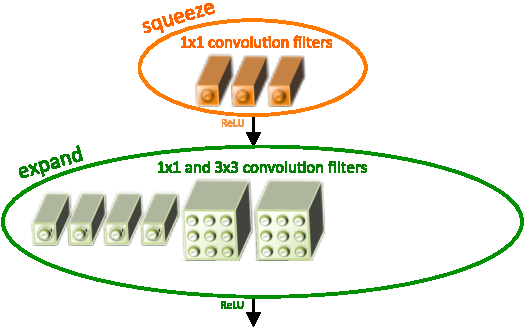
\includegraphics[width=\textwidth, height=0.3\textheight, keepaspectratio]{squeeze.pdf}
        \caption{Squeezenet Fire Module\cite{iandola_squeezenet_2016}}
        \label{fig:archi_building_block:sqn}
    \end{subfigure}
    %
    \begin{subfigure}[t]{0.49\linewidth}
        \centering
        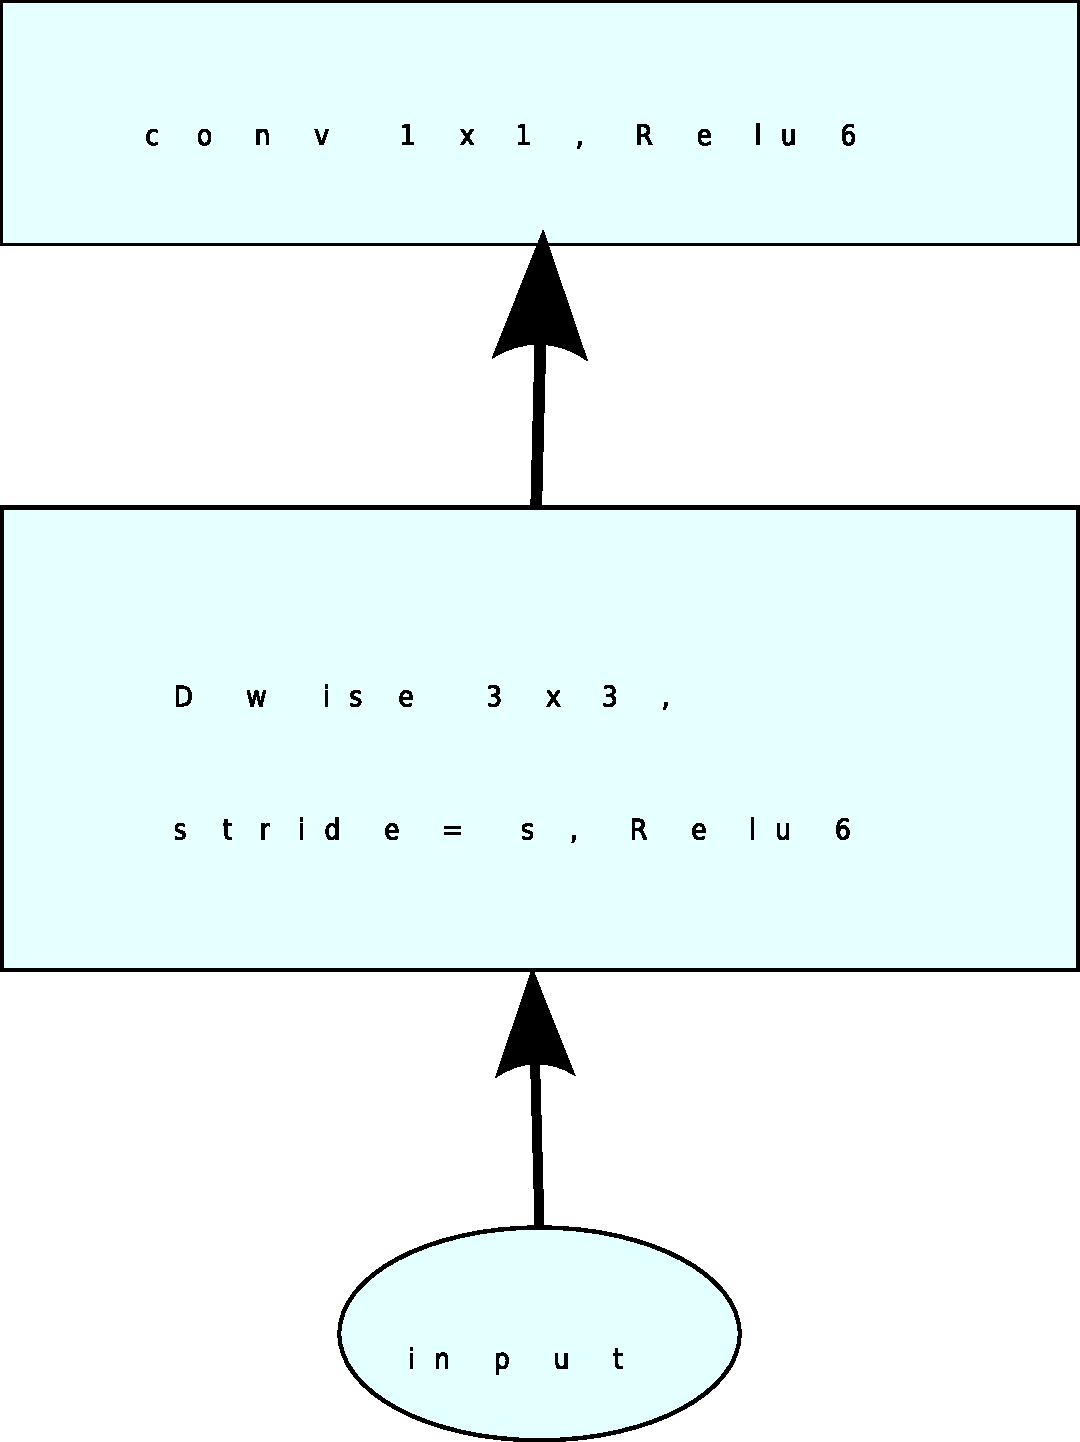
\includegraphics[width=\textwidth, height=0.2\textheight, keepaspectratio]{mobilenet.pdf}
        \caption{MobileNet convolutional block \cite{howard_mobilenets_2017}}
        \label{fig:archi_building_block:mbn}
    \end{subfigure}
    %
    \begin{subfigure}[t]{0.49\linewidth}
        \centering
        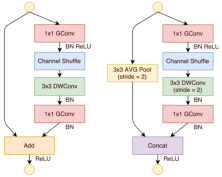
\includegraphics[width=\textwidth, height=0.2\textheight, keepaspectratio]{shufflenet.pdf}
        \caption{ShuffleNet convolutional block \cite{zhang_shufflenet_2018}}
        \label{fig:archi_building_block:shn}
    \end{subfigure}
    %
    \begin{subfigure}[t]{0.49\linewidth}
        \centering
        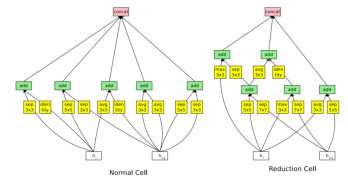
\includegraphics[width=\textwidth, height=0.3\textheight, keepaspectratio]{nasnet.pdf}
        \caption{NasNet convolutional blocks \cite{zoph_learning_2018}}
        \label{fig:archi_building_block:nasn}
    \end{subfigure}
    %
    \begin{subfigure}[t]{0.49\linewidth}
        \centering
        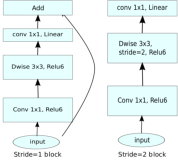
\includegraphics[width=\textwidth, height=0.2\textheight, keepaspectratio]{mobilenet2.pdf}
        \caption{MobileNetv2 convolutional blocks \cite{sandler_mobilenetv2_2018}}
        \label{fig:archi_building_block:mb2n}
    \end{subfigure}
    %
    \caption{Convolutional block from different architectures}
    \label{fig:archi_building_block}
\end{figure}

The architecture used in this work was developed to implement MobileNetV2 because of its simplicity and its state-of-the-art performance (see Table \ref{tab:mbv2}). Moreover, MobileNetV2 requires fewer parameters while providing state-of-the-art accuracy when comparing to the different architectures, as shown in Figure \ref{fig:archi}.
%
\begin{table}[H]
    \center
    \begin{tabular}{ | c | c | c c | c| }
        \hline \hline
        Network & Top 1 & Params & MAdds & CPU \\
        \hline \hline
        MobileNetV1 & 70.6 & 4.2M & 575M & 113ms \\
        ShuffleNet (1.5) & 71.5 & \textbf{3.4M} & 292M & - \\
        ShuffleNet (x2)  & 73.7 & 5.4M & 524M & - \\
        NasNet-A & 74.0 & 5.3M & 564M & 183ms \\
        \hline
        MobileNetV2 & \textbf{72.0} & \textbf{3.4M} & \textbf{300M} & \textbf{75ms} \\
        MobileNetV2 (1.4) & \textbf{74.7} & 6.9M & 585M & \textbf{143ms} \\
        \hline \hline
    \end{tabular}
    \caption{Performance on ImageNet, comparison for different networks \cite{sandler_mobilenetv2_2018}}
    \label{tab:mbv2}
\end{table}

\begin{figure}[H]
    \centering
    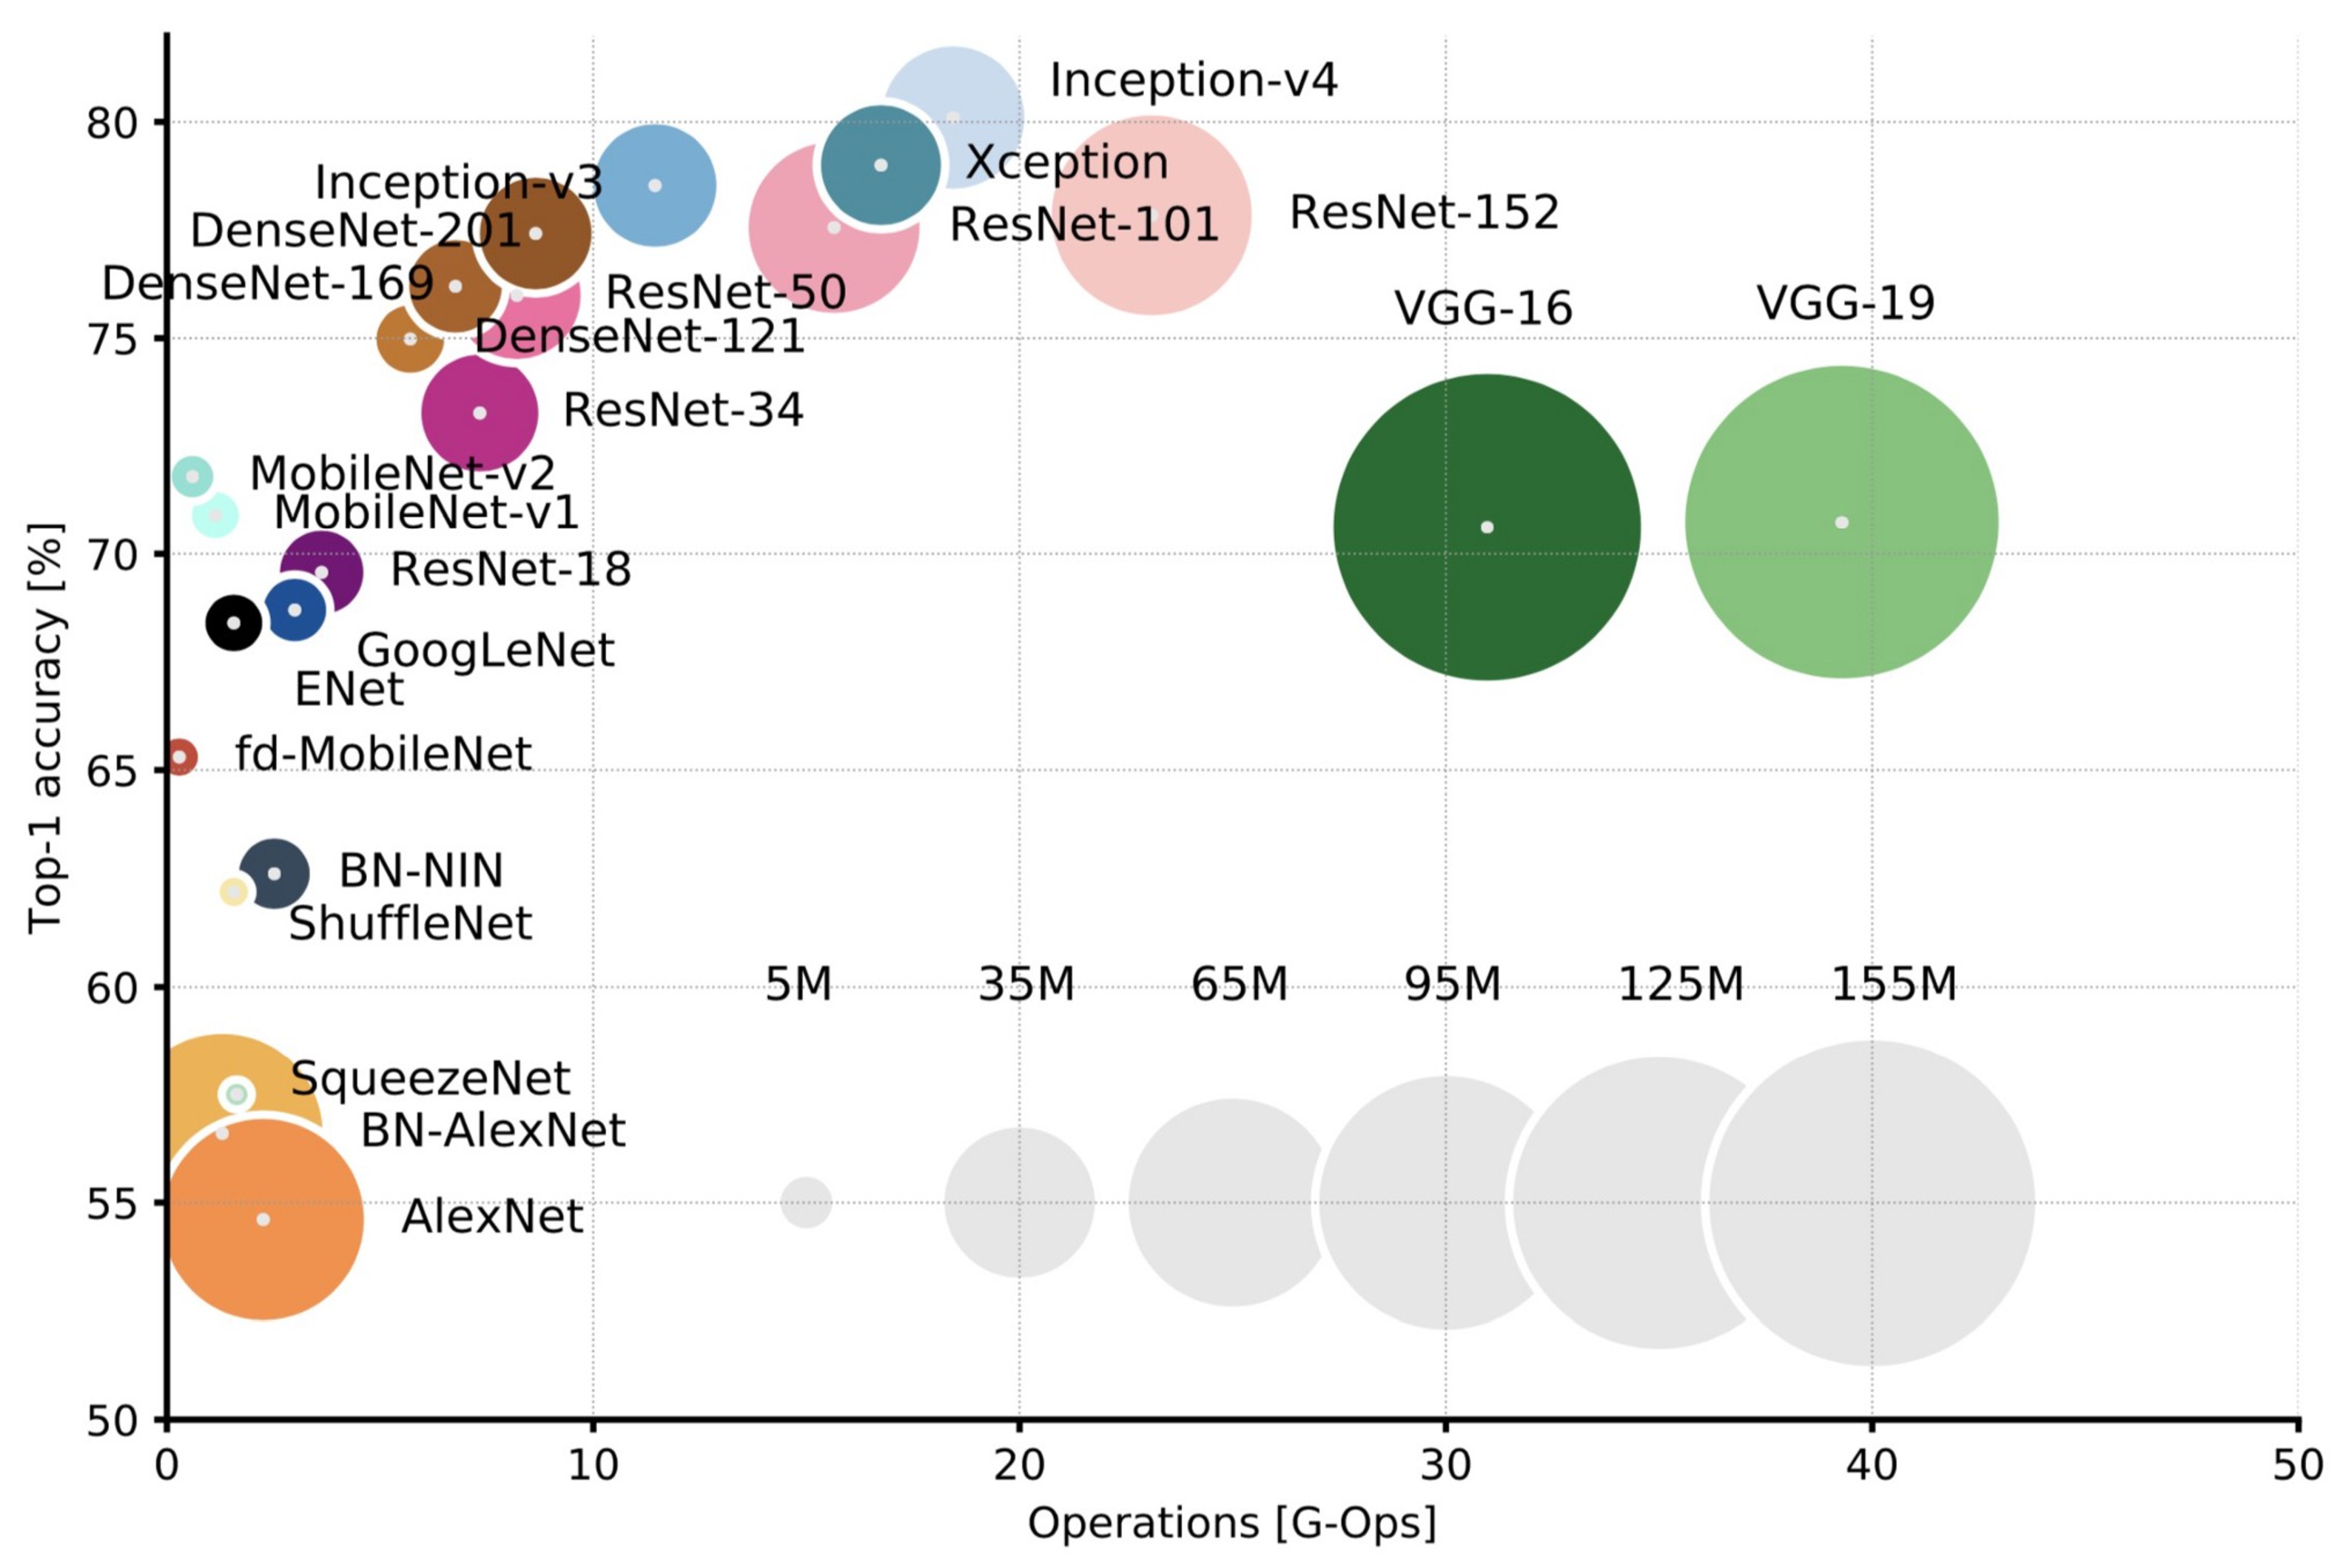
\includegraphics[width=0.9\textwidth]{archi.pdf}
    \caption{Ball chart reporting the Top-1 accuracy of various architectures vs. their computational complexity \cite{canziani_analysis_2017}}
    \label{fig:archi}
\end{figure}
%
\subsubsection{Pruning} \label{subs:pruning}
%
To improve the inference phase of a \acrshort{cnn}, pruning can be used, especially for platforms with limited computational resources \cite{liu_rethinking_2019}. According to \textcite{liu_rethinking_2019, denton_exploiting_2014}, the huge number of parameters in a network might create a problem of \textbf{over-parametrization}. Over-parametrization means that there are redundancies in \acrshort{nn} parameters and that the same performance could be achieved with only a subset of them. In other words, a lot of parameters are unimportant or unnecessary \cite{cheng_recent_2018}. Pruning is defined as removing the parameters considered as not important. For example, \textcite{baoyuan_liu_sparse_2015} achieve more than 90\% sparsity of parameters in convolutional layers in AlexNet with less than 1\% accuracy loss.

We can explain why pruning works by \textbf{The Lottery Ticket Hypothesis} \cite{frankle_lottery_2018, frankle_early_2020}: \textquote{\textit{A randomly initialized, dense neural network contains a subnetwork that is initialized such that—when trained in isolation—it can match the test accuracy of the original network after training for at most the same number of iterations.}} From this postulate, those unimportant weights can be set to zero (prune) because they do not improve the accuracy of the model.

According to \textcite{cheng_recent_2018}, pruning has two major benefits for the inference phase. First, less storage is required. Indeed, the non-pruned weights are sparsely distributed among the kernels. Thus, they can be stored in a compressed format reducing memory utilization. Second, pruning reduces the arithmetic complexity of the network. As convolutions perform a weighted sum with the input \acrshort{fm}, each \acrfull{mac} operation with a pruned weight can be discarded. Moreover, \textcite{han_learning_2015, mao_exploring_2017, kang_accelerator-aware_2020} pointed out that some pruning ratios can also improve the accuracy of the network, which can be explained by a form of regularization.

Various pruning schemes are focused on increasing the sparsity of the network without a drop of accuracy \cite{han_deep_2016, han_learning_2015}.  We call this pruning scheme where all unimportant parameters are pruned without extra constraint \textbf{unstructured pruning} \cite{cheng_recent_2018}. However, it is challenging to exploit the performance and the high parallelism of \acrshort{fpga} with this kind of pruned network. Indeed, this kind of pruning scheme creates irregularities in the data access pattern \cite{zhu_efficient_2020}. It means that the number of pruned weights is different in each kernel, and we should adapt the circuitry to the worst case. As a consequence, all filters conduct wasteful operations except the worst case \cite{shimoda_filter-wise_2019}. Furthermore, \textcite{anwar_structured_2017} pointed out that unstructured pruning requires overhead for computing addresses of the sparse non-pruned elements. Therefore, we should find pruning patterns that would be more hardware-friendly.

In contrast to the unstructured pruning, we have \textbf{structured pruning} schemes \cite{kang_accelerator-aware_2020}. They combine a structure regularization for accuracy and locality optimization for computation efficiency. According to \textcite{anwar_structured_2017}, \textquote{\textit{Structured pruning has no or little extra costs}}. We can categorize the various schemes into different groups \cite{cheng_recent_2018, kang_accelerator-aware_2020, anwar_structured_2017, wen_learning_2016}:
\begin{itemize}
    \item \textbf{Depth-wise}: all the weights of a layer are pruned. The layer is then removed.
    \item \textbf{Kernel-wise}: instead of pruning all the weights, we keep a ratio of kernels, which means a reduction of the number of output channels. This pruning scheme is provided in Figure \ref{fig:struct_pruning:fw}.
    \item \textbf{Channel-wise}: it is one of the most popular methods because it still can fit in the convolutional deep learning frameworks \cite{liu_rethinking_2019}. A layer of the input \acrshort{fm} is pruned, which means that the layer is also pruned in all the kernels, as can be seen in Figure \ref{fig:struct_pruning:chw}.
    \item \textbf{Shape-wise}: we prune the same weights in each kernel or group of kernels. For example, this pruning scheme was used in \textcite{zhu_efficient_2020}. It is illustrated in Figure \ref{fig:struct_pruning:sw}
\end{itemize}
%
\begin{figure}[H]
    \centering
    %
    \begin{subfigure}[t]{.32\textwidth}
    \centering
    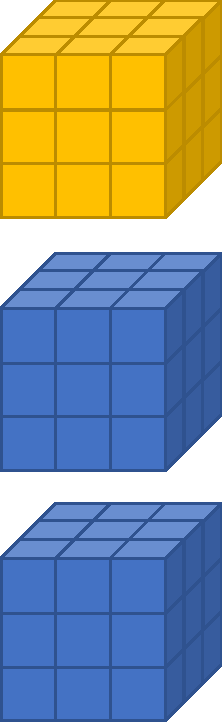
\includegraphics[width=0.33\linewidth]{filterwise.pdf}
    \caption{kernel-wise pruning}
    \label{fig:struct_pruning:fw}
    \end{subfigure}
    %
    \begin{subfigure}[t]{.32\textwidth}
    \centering
    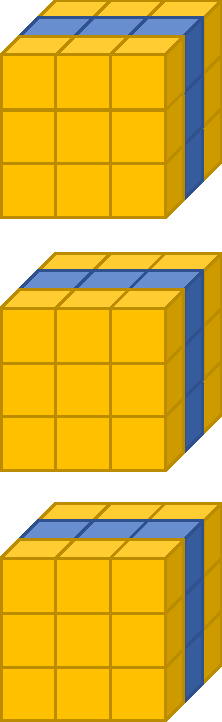
\includegraphics[width=0.33\linewidth]{channelwise.pdf}
    \caption{channel-wise pruning}
    \label{fig:struct_pruning:chw}
    \end{subfigure}
    %
    \begin{subfigure}[t]{.32\textwidth}
    \centering
    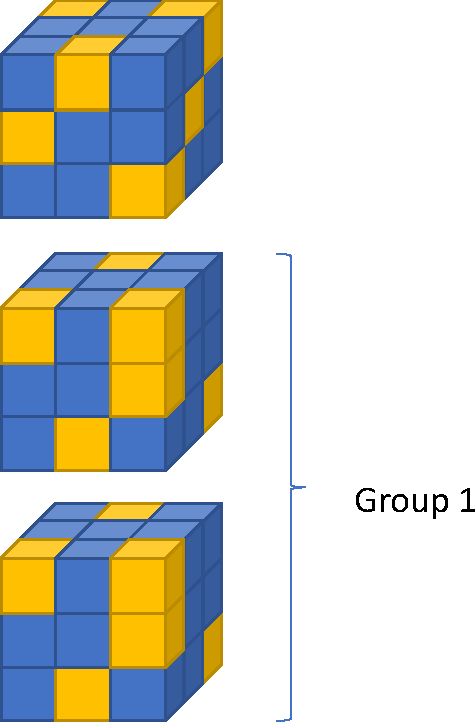
\includegraphics[width=0.70\linewidth]{shapewise.pdf}
    \caption{shape-wise pruning}
    \label{fig:struct_pruning:sw}
    \end{subfigure}
    %
    \caption{Structured pruning schemes, where the yellow weights are the pruned ones, inspired by \cite{cheng_recent_2018}}
    \label{fig:struct_pruning}
\end{figure}
%
The previously cited pruning schemes are ordered from very coarse-grained to fine-grained sparsity \cite{mao_exploring_2017}. As explained previously, coarse-grained sparsity (channel-wise and filter-wise pruning) provides a higher acceleration and can be used when implementing \acrshort{cnn} on \acrshort{gpu} or \acrshort{cpu} \cite{cheng_recent_2018, mao_exploring_2017}. However, finer-grained ones provide higher accuracy and as the sparsity increases, the accuracy is less affected, as can be seen in Figure \ref{fig:pruning-accuracy}. Therefore, this work focuses on developing customized hardware that can exploit a more fine-grained sparsity \cite{mao_exploring_2017} to provide a higher pruning while limiting the drop of accuracy.
%
\begin{figure}[H]
    \centering
    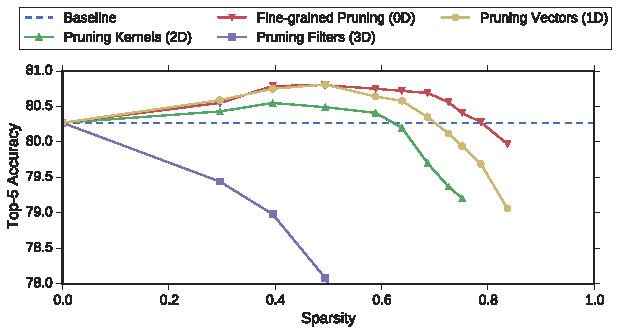
\includegraphics[width=\textwidth]{accuracysparsity.pdf}
    \caption{Accuracy-Sparsity Curve of AlexNet obtained by pruning \cite{mao_exploring_2017}}
    \label{fig:pruning-accuracy}
\end{figure}
%
Some studies focused on the acceleration of the inference step of lightweight models thanks to pruning. \textcite{zhang_channel_2019, tu_pruning_2019} applied pruning on \acrshort{dsc} kernels. They both chose \textbf{Channel-wise} pruning because it does not create sparse connections and it efficiently improves the speed of the inference. It also reduces the computational cost of the $1 \times 1$ (pointwise) convolutions, which has the biggest number of parameters and computational complexity. In MobileNet, it is about 95\%. By discarding one channel, the associated depthwise convolution is also avoided.
Moreover, the pointwise kernel producing that channel in the previous block can also be pruned. We can see the process in Figure \ref{fig:pruning_dsc}.
%
\begin{figure}[H]
    \centering
    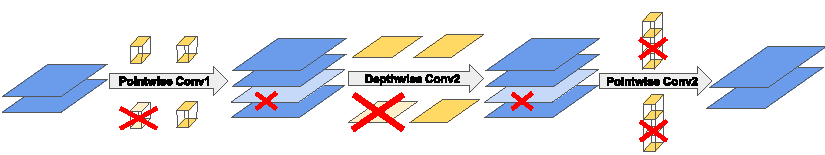
\includegraphics[width=\textwidth]{channelwise_ex.pdf}
    \caption{Pruning a depthwise separable convolution \cite{tu_pruning_2019}}
    \label{fig:pruning_dsc}
\end{figure}

\textbf{In this work, we focus on a structured pruning scheme for depthwise separable convolution. More precisely, we develop an architecture on \acrshort{fpga} than combines both advantages of pruning and depthwise separable convolution.}
%
\subsubsection{Quantization} \label{subs:quantization}
%
%
Quantization is an approach to trade accuracy for a decrease of the storage requirements of a network \cite{han_deep_2016}. Indeed, we can define quantization as the reduction of the number of bits representing a weight or pixel. Moreover, instead of using a floating-point number, we can use a \textbf{fixed-point number} \cite{cheng_recent_2018}. As said previously, fixed-point numbers are known to be more efficient on hardware such as \acrshort{fpga} because we can use integer arithmetic \cite{david_hardware_2007}. Quantization to fixed-point numbers can then reduce the memory requirement and the latency of the inference stage.

The format to encode the fixed-point representation of a real number is the \textit{Q-format} \cite{ward_real-time_2001}. A N-bit number, noted $Q_{m.n}$, is divided into two parts separated by an implied binary point. The $m$ bits are used to represent the integer part of the number (including the sign bit), and the $n$ bits are used to represent the fractional part, as can be seen in Figure \ref{fig:Qformat}. The bitwidth associated with each part can be either the same, either fine-tuned for each layer after analysis. Indeed, \textcite{qiu_going_2016, yin_high_2018} choose a different range for each layer, but doing it for every weight is not memory-efficient.
%
\begin{figure}[H]
    \centering
    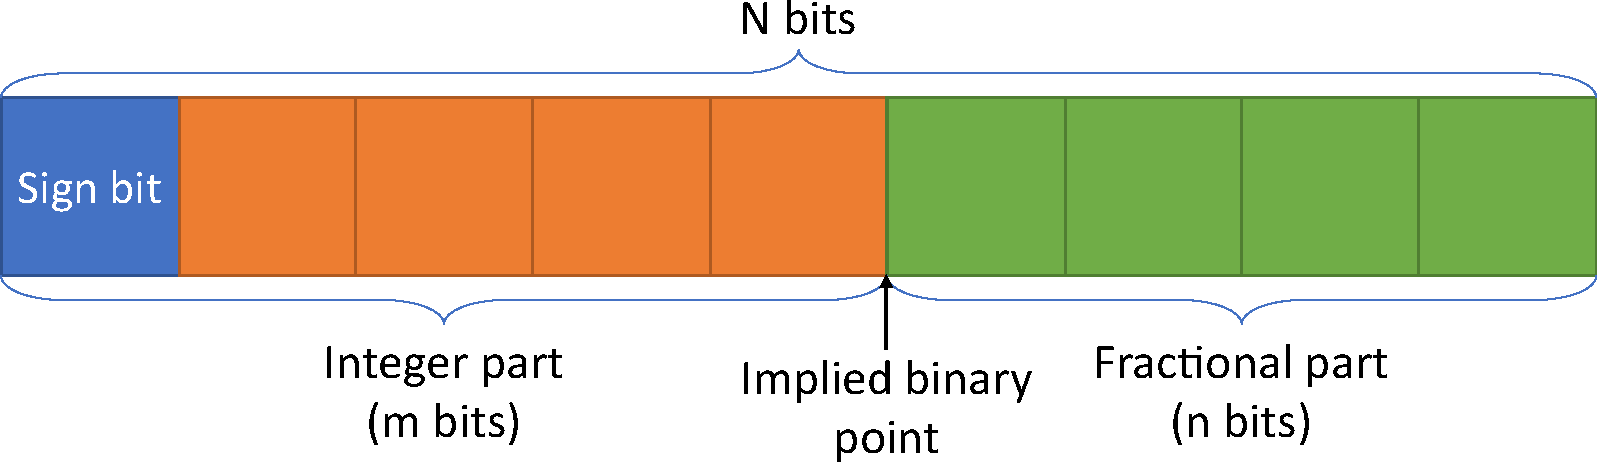
\includegraphics[width=\textwidth]{Qformat.pdf}
    \caption{Illustration of the Q-format}
    \label{fig:Qformat}
\end{figure}

As pointed out by \textcite{han_deep_2016}, quantization and pruning techniques are orthogonal and can be combined to compress further the network. Unfortunately, not all existing networks are friendly for quantization, like MobileNet. MobiletNet with quantized pixels and weights has a large drop of accuracy compared with its Non-quantized version (70.50\% using floating-point model vs 1.80\% using an 8-bit pipeline) \cite{sheng_quantization-friendly_2018}. However, the work of \textcite{sheng_quantization-friendly_2018} showed that the source of the accuracy drop was the design of the separable convolution core layer. They proposed therefore a new quantization-friendly separable convolution core layer. Works on MobileNetV2 should then be done to verify the fixed-point inference accuracy. Still, an 8-bit pipeline might not be optimal for MobilNetV2 as increasing the bitwidth to 16-bit could boost accuracy \cite{cheng_recent_2018}. This bitwidth is also widely used \cite{huimin_li_high_2016, bai_cnn_2018}. 

\textbf{Therefore, 16-bit fixed-point Q-format is adopted for input data, weights, and intermediate data in the frame of this thesis}. \textbf{Moreover, as said previously in Section \ref{subs:acti}, we can limit the integer part to 3 bits (one bit is added to express the sign of the weights), and we can use $Q_{4.12}$.}

%%%%%%%%%%%%
\section{Conclusion} \label{sec:cclopti}
We can observe on table that pruning seem to be a preferable solutions because ... \newline \newline
On next chapter we are going to explore how to handle pruning on \acrshort{fpga}.


%
\begin{tcolorbox}
    \textbf{Conclusion about the State of the Art}: \newline \newline

    We knew from the previous chapter that the most performing models have a huge computational complexity and memory utilization, which limit the implementation of such models on mobile platforms, such as \acrshort{fpga}. Therefore, we reviewed the literature to find optimizations that allow an efficient implementation of \acrshort{cnn}s on \acrshort{fpga}. We have explored algorithmic optimizations, but they only reduce the computational complexity while increasing hardware utilization. Model optimizations seem to be more relevant because they aim at reducing both the number of parameters and operation in exchange for a drop of accuracy. Therefore, we can investigate the combination of different optimizations to further compress models, like pruning and quantization. \newline \newline
    
    As a result, this work focus on developing a pruning scheme on \acrshort{dsc} to see if their gain can be combined. To study the performance of the proposed pruning scheme, we use it on a state of the art model that contains \acrshort{dsc}: MobileNetV2. Moreover, as quantizing is an orthogonal approach to pruning, we also use fixed-point formats to accelerate further the inference of the architecture. We chose 16-bit because the loss of accuracy can be controlled.
\end{tcolorbox}
\afterpage{\blankpage}
\cleardoublepage
\newpage

	
	%% Part 3
	\chapter{Accelerating Convolutional Neural Networks for FPGA using Depthwise Separable Convolution and Pruning} \label{chap:pratique}
%
%
In the previous chapter, we introduced pruning, which reduces both size and computational complexity of \acrshort{cnn}s. We also showed that there exist various pruning schemes. Each of them can be categorized from coarse-grained to fine-grained. Coarse-grained pruning schemes have the advantage that they can be easily implemented on \acrshort{gpu} and \acrshort{cpu} in exchange for a drop of accuracy. On the other hand, fine-grained pruning schemes can limit this reduction of accuracy but can create irregular access pattern that makes them difficult to implement on such platforms. 

To have an efficient \acrshort{fpga}-based accelerator, we should focus on implementing the most fine-grained pruning scheme possible to apply a high sparsity while limiting the loss of accuracy. This shows the advantage of using \acrshort{fpga} accelerator because, as said previously, this type of pruning scheme is not easily implementable on \acrshort{cpu} and \acrshort{gpu}

In this chapter, we define an \acrshort{fpga}-based accelerator architecture that integrates both pruning and \acrshort{dsc} (see Section \ref{subs:dsc}) to reduce the number of weights and operations. To show its applicability, this architecture implements a state-of-the-art network that includes \acrshort{dsc} and targets an embedded platform: MobileNetV2 (Sections \ref{subs:mbv2} and \ref{subsec:mdopti}). Since the pruning can cause degradation of the performance, we have to determine the design objectives of the architecture and its associated pruning scheme, which are the following:
%
\begin{enumerate}
    \item The pruning scheme is as fine-grained as possible.
    \item The pruning scheme reduces the computational complexity.
    \item The pruning scheme allows for a reduction of the memory required to store the weights.
    \item The proposed architecture provides a logically correct output.
    \item An increase in the sparsity improves the performance of the architecture.
\end{enumerate}

Moreover, the \acrshort{fpga}-based accelerator architecture is implemented on a Cyclone V \acrshort{fpga}.

Section \ref{sec:design} aims at developing the pruning scheme and the algorithm to handle it. We also define in this section the weight and operation reduction factors obtained when applying the proposed pruning scheme. We also define a weight compressed format to reduce weight memory use. We then perform a loop analysis on the proposed algorithm to determine the optimal hardware design variables and the structure of the architecture.

Section \ref{sec:implementation} describes the implementation of the \acrshort{fpga}-based accelerator architecture and details its dataflow. We start by explaining the overall architecture and then we go in more details into each of its components.

Section \ref{sec:measure} shows the results obtained and discusses if the proposed design objectives are met.
%
\section{Design of a FPGA-based accelerator integrating structured sparse DSC} \label{sec:design}
%
As previously said,  the aim of this section is to develop a pruning scheme for the \acrshort{dsc} that fulfills the design objectives and an algorithm able to support it. First, we detail the pruning scheme used and the weights and operations reduction factors obtained by applying the pruning. Second, we analyse the sparse kernels to find a compressed format that reduces the memory use and overhead of determing the address of the non-pruned weights. Third, we describe the algorithm proposed to perform the sparse \acrshort{dsc} using the proposed pruning scheme. Finally, we analyse the convolution loops to determine the optimal design of the \acrshort{pe} that perfoms the convolution.
%
\subsection{Pruning scheme} \label{subsec:pscheme}
%
\acrshort{dsc} is composed of two types of convolution: depthwise and pointwise convolutions (see Section \ref{subsec:layer}). We decided to apply pruning on the pointwise filters for the following reasons:
%
\begin{itemize}
    \item In MobileNet and MobileNetV2, most of the operations are done in the pointwise convolutions \cite{zhang_channel_2019, tu_pruning_2019}. So it is the operation where the reduction of weights and computational complexity would be the most relevant (each operation requires one weight).
    \item As each kernel of pointwise filter is a vector of size $1 \times 1  \times N_{if}$, we therefore have to prune in the channel-axis. This scheme was proven to be successful by \textcite{kang_accelerator-aware_2020}.
    \item The pruning scheme can be applied to each $1 \times 1$ convolution in the network.
\end{itemize}
%
As mentionned above, we decided to develop a pruning scheme inspired by the methodology of \textcite{kang_accelerator-aware_2020}, which prunes weights in the channel-axis.

Ideally, without pruning, each \acrshort{pe} performing a pointwise convolution fetches $N_{if}$ weights and input pixels belonging to spatial coordinates $(x, y)$ (pointwise convolution only convolves pixels in the channel-axis). Then each weight is multiplied with its corresponding pixel and the products are summed to obtain one output pixel of one channel. If we apply an unstructured pruning on the pointwise filter, we can use the same algorithm as above but only each non-pruned weight is multiplied with its corresponding pixel (multiplication implying zero-value weights can be safely discarded).

However, as the resources of the \acrshort{fpga} are limited, the \acrshort{pe} can only fetch $N_{par} \leq N_{if}$ weights and pixels at each time (which corresponds to a \textbf{fetching group}; each input \acrshort{fm} and kernel are composed of $N_{gr}$ fetching groups). Therefore, we would do the convolution between each fetching group and accumulate the different partial sums belonging to a same output pixel until an output pixel is produced. If an unstructured pruning is applied, this can cause several issues, as pointed out by \cite{kang_accelerator-aware_2020}.

First, it can cause misalignement between the weight and pixel fetching groups. Indeed if we prune the first $N_{par}$ weights in the kernel, the first pixel fetching group is useless. Second, there can be a load-imbalance problem (see Section \ref{subsec:impl_prun}) that can occur between two \acrshort{pe}s if the number of pruned weights between two kernels is different. 

To solve these problems, the solution proposed by \textcite{kang_accelerator-aware_2020} is to align pixel and weight fetching groups. Each pixel fetching group has a corresponding weight fetching group containing at least one non-pruned weight. \textcite{kang_accelerator-aware_2020} also constrains the number of non-pruned weights in each fetching group to be the same number, called $N_{np}$. Therefore, it solves also the load-imbalance problem. As a result, the proposed sparse \acrshort{dsc} can be illustrated in Figure \ref{fig:prunedwg}.
%
\begin{figure}[H]
    \centering
    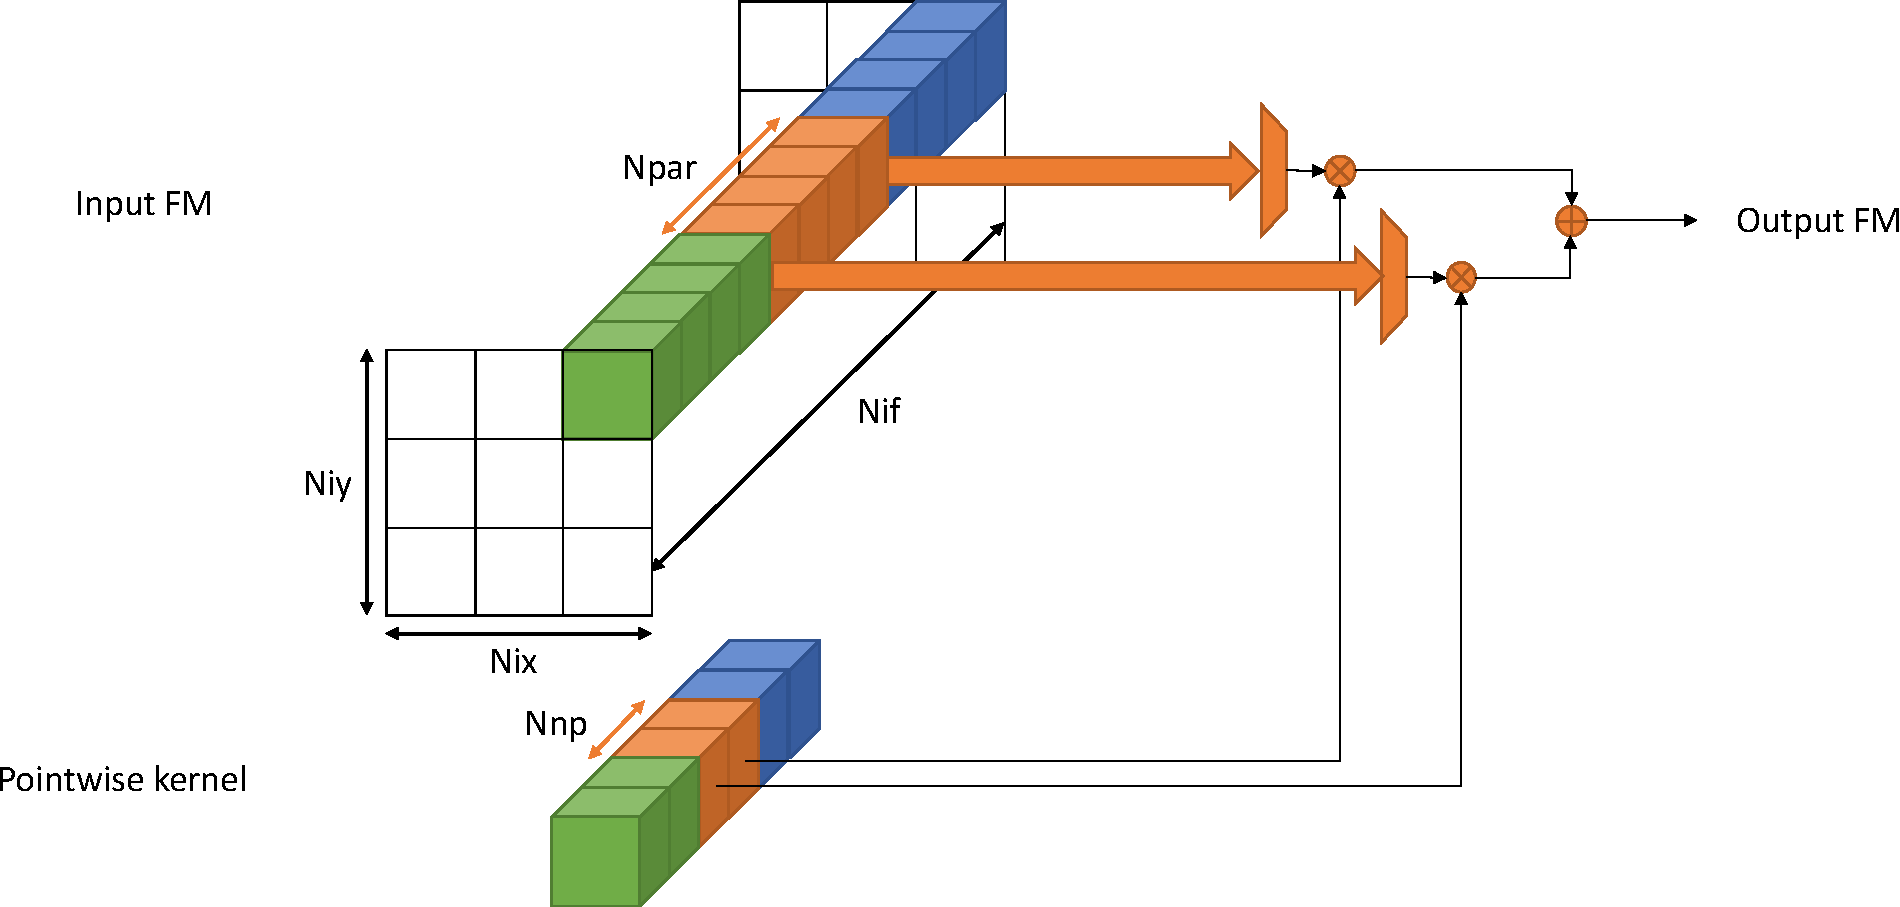
\includegraphics[width=\textwidth]{pruningscheme.pdf}
    \caption{Process of a pointwise convolution with a sparse pointwise kernel, inspired by \cite{kang_accelerator-aware_2020}}
    \label{fig:prunedwg}
\end{figure}
%
To summarize, each pointwise kernel is composed of $N_{gr}$ fetching groups of $N_{np}$ weights. Each group corresponds to a pixel fetching group of size $N_{par}$. We define the ratio between the number of non-pruned weights and the size of the fetching group without pruning as the \textbf{pruning ratio $\alpha$}, the number of weights remaining after pruning. The ratio of pruned weights is therefore equal to $1 - \alpha$. The pruning parameters are defined in Table \ref{tab:pr_param}. Moreover, the proposed pruning scheme can also be applied to each $1 \times 1$ kernels.
%
\begin{table}[H]
    \center
    \begin{tabular}{|c|c|c|}
        \hline
        $N_{par}$ & The input pixel fetching group size. & $N_{par} \leq N_{if}$ \\
        \hline
        $N_{np}$  & The pointwise weight fetching group size. & $N_{np} \leq N_{par}$ \\
        \hline
        $N_{gr}$  & The number of fetching groups & $N_{gr} = \left\lceil \frac{N_{if}}{N_{par}} \right\rceil $ \\
        \hline
        $\alpha$  & The pruning ratio & $\alpha = \frac{N_{np}}{N_{par}}  $ \\
        \hline
    \end{tabular}
    \caption{Pruning parameters}
    \label{tab:pr_param}
\end{table}
%
We should add that this pruning scheme is not the same as \textit{channel pruning} since we do not constrain the same weights to be pruned in each group. Therefore, I did not consider the pruning of the depthwise kernel associated to the pruning of a weight in each kernel, as discussed in Section \ref{subs:pruning}. We have then proposed a pruning-scheme that is not coarse-grained (channel pruning), satisfying first design objective: \textbf{\textquote{The pruning scheme is as fine-grained as possible}}.
%
\subsubsection{Reduction factors}
%
We can now evaluate the reduction factors of the sparse \acrshort{dsc} compared with the \acrshort{dsc} without pruning and the standard convolution.

We consider that the size of the input feature map of the pointwise convolution is $N_{ix}  \times N_{iy} \times N_{if}$, the size of the depthwise filter is $N_{kx} \times N_{ky} \times N_{if}$, the size of the non-pruned pointwise convolution $N_{if} \times N_{of}$, the fetching group size is $N_{par}$, the number of pruned weights is $N_{np}$, and the size of the output \acrshort{fm} is $N_{ox}  \times N_{oy} \times N_{of}$. The amount of weights $W_{DSC}$ and operations $O_{DSC}$ of the \acrshort{dsc} can be determined using Equation \eqref{eq:dsc_wg} and \eqref{eq:dsc_op} \cite{bai_cnn_2018, liu_fpga-based_2019}.
%
\begin{equation}
    W_{DSC} = N_{kx} \times N_{ky} \times N_{if} + N_{if} + \times N_{of}
    \label{eq:dsc_wg}
\end{equation}
%
\begin{equation}
    O_{DSC} = N_{ix} \times N_{iy} \times N_{kx} \times N_{ky} \times N_{if} + N_{ix} \times N_{iy} \times N_{if} \times N_{of}
    \label{eq:dsc_op}
\end{equation}

In a same manner, the amount of weights $W_{PR\_DSC}$ and operations $O_{PR\_DSC}$ of the sparse \acrshort{dsc} can be determined using Equation \eqref{eq:pr_dsc_wg} and \eqref{eq:pr_dsc_op}.
%
\begin{equation}
    W_{PR\_DSC} = N_{kx} \times N_{ky} \times N_{if} + \times N_{if} + N_{np} \times N_{gr} \times N_{of}
    \label{eq:pr_dsc_wg}
\end{equation}
%
\begin{equation}
    O_{PR\_DSC} = N_{ix} \times N_{iy} \times N_{kx} \times N_{ky} \times N_{if} + N_{ix} \times N_{iy} \times N_{gr} \times N_{np} \times N_{of}
    \label{eq:pr_dsc_op}
\end{equation}

Thus, the weights $F_{Wg}$ and operations $F_{Op}$ reduction factors can be expressed according to Equation \eqref{eq:factor_comp_wg} and \eqref{eq:factor_comp_op}. The demonstration allowing to find these relations can be found in Appendix \ref{appendix:factor}.
%
\begin{equation}
    F_{Wg} = \frac{W_{DSC}}{W_{PR\_DSC}} = \frac{1 + \frac{N_{kx} \times N_{ky}} {N_{of}}} {\alpha + \frac{N_{kx} \times N_{ky}} {N_{of}}}
    \label{eq:factor_comp_wg}
\end{equation}
\begin{equation}
    F_{Op} = \frac{O_{DSC}}{O_{PR\_DSC}} = \frac{1 + \frac{N_{kx} \times N_{ky}} {N_{of}}} {\alpha + \frac{N_{kx} \times N_{ky}} {N_{of}}}
    \label{eq:factor_comp_op}
\end{equation}

As the reduction factors depend on the pruning ratio $\alpha$ and the number of output channels $N_{of}$, we can illustrate the evolution of the reduction factors depending on this parameter and the different $N_{of}$ of MobileNetV2. This can be seen in Figure \ref{fig:redfacto}.
%
\begin{figure}[H]
    \centering
    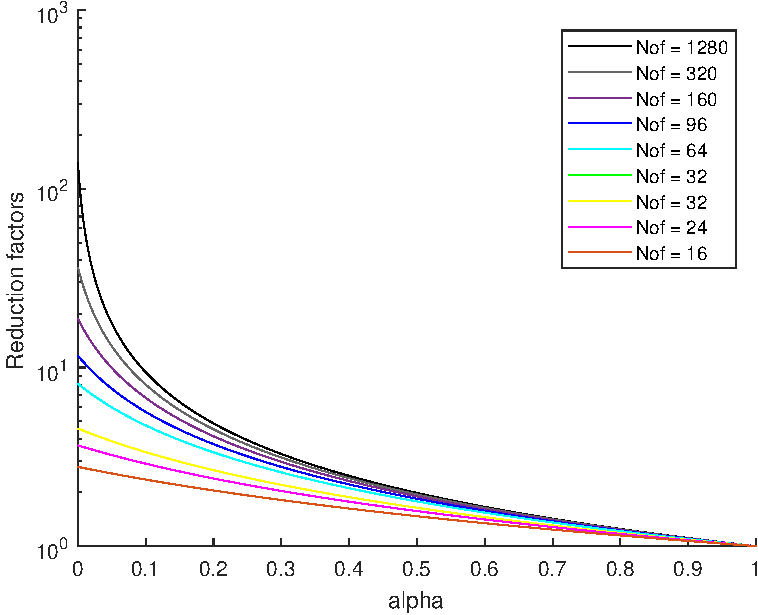
\includegraphics[width=0.75\textwidth]{RedFactor.pdf}
    \caption{Evolution of the reduction factors depending on the pruning ratio and the number of output channel}
    \label{fig:redfacto}
\end{figure}

For example, if we apply a pruning ratio of $25\%$ (meaning keeping $25\%$ of the weights in each fetching group), the reduction factors compared the \acrshort{dsc} without pruning are between two and four times. If we consider the reduction factor between \acrshort{dsc} and standard convolution is about 9 times \cite{zhang_channel_2019}, the reduction factors between sparse \acrshort{dsc} and standard convolution is between 18 and 36 times (if $\alpha = 25\%$). We therefore validated the second design objective, which is: \textbf{\textquote{The pruning scheme reduces the computational complexity}}.
%
\subsection{Compressed format} \label{subs:compress_f}
%
After applying the pruning scheme on the pointwise kernels, these kernels become sparse. This means that they contain zero-value weights, as illustrated in Figure \ref{fig:pruned_wg}. Therefore, in order to reduce the memory usage, we should only store each non-pruned weights in a compressed format that allows finding its address with no extra-overhead.
%
\begin{figure}[H]
    \centering
    \includegraphics[width=0.75\textwidth]{pruned_wg.pdf}
    \caption{A pointwise kernel after pruning, where black cubes are pruned weights}
    \label{fig:pruned_wg}
\end{figure}

A conventional storage format for sparse matrix is the \acrfull{csr} \cite{buluc_parallel_2009}. According to \textcite{buluc_parallel_2009}, \textquote{\textit{The compressed sparse row (CSR) format stores the nonzeros (and ideally only the nonzeros) of each matrix row in consecutive memory locations,  and  it  stores  an  index  to  the  first  stored  element of each row}}. In other words, we represent a sparse matrix using three vectors:
%
\begin{itemize}
    \item \textbf{Vector val}: containing all the values of the non-pruned weights.
    \item \textbf{Vector col\_ind}: contains the column indices of the elements in \textbf{val}.
    \item \textbf{Vector row\_ptr}: contains the index of each row in \textbf{val}.
\end{itemize}
%
However, as for \cite{zhu_efficient_2020}, the \acrshort{csr} format can be compressed further thanks to the pruning scheme. Indeed, since the kernels to compress are vectors, we can reduce the storage usage by removing the \textbf{row\_ptr} vector (the kernel has only one row). 

Moreover, we can have a better compression if we reduce the number of bits allocated to represent the column index of a weigth. Indeed, without pruning, as each weight belongs in a fetching group of size $N_{par}$, it is sufficient to store the position of the weight in that group, instead of its asbolute position in the kernel. As a result, we can reduce the number of bits from $log_2(N_{if})$ (asbolute position) to $log_2(N_{par})$ (relative position), where $N_{par} \leq N_{if}$. Moreover, it also reduces the overhead to find the corresponding pixel in a fetching group, for each weight.

In brief, each sparse kernel is converted into 2 vectors of size $N_{np}$: vector \textbf{val}, which contains the value of the non-pruned weights, and vector \textbf{position}, which contains the position of the corresponding pixel in a fetching group. An example is illustrated in figure \ref{fig:compressed_format}.
%
\begin{figure}[H]
    \centering
    \includegraphics[width=0.75\textwidth]{compressed_format.pdf}
    \caption{Illustration of the compressed format on an example, where $N_{par} = 4$ and $N_{np} = 2$}
    \label{fig:compressed_format}
\end{figure}

Since this compressed format requires an extra position per weight (and hence more bits allocated per weight), we computed the maximal pruning ratio, or in a same way the minimal ratio of pruned weights, required to have a reduction of the memory usage. The relation between maximal pruning ratio and memory reduction can be found in Equation \eqref{eq:prun_mem} where $BW_{weight}$ is the bitwidth required to represent the value of a weight. The demonstration to find the maximal pruning ratio $\alpha$ to reduce the memory usage can be found in Appendix \ref{appendix:cf}.
%
\begin{equation}
    \alpha < \frac{BW_{weight}}{ BW_{weight} + log_2(N_{par})}
    \label{eq:prun_mem}
\end{equation}

The curve representing the minimal ratio of pruned weight, equals to $1 - \alpha$, depending on $N_{par}$ when $BW_{weight} = 16$ is illustrated in Figure \ref{fig:prun_mem}. We can conclude from the curve that we need to have a ratio of pruned weights to be greater or equal than $40\%$ in order to save memory. We can also conclude that we can prune less weights if we reduce the value of $N_{par}$. We therefore validated the third design objective, which is: \textbf{\textquote{The pruning scheme allows a reduction of the memory required to store the weights}}.
%
\begin{figure}[H]
    \centering
    \includegraphics[width=0.75\textwidth]{MinCompr.pdf}
    \caption{Minimal ratio of pruned weights if $BW$ = 16}
    \label{fig:prun_mem}
\end{figure}
%
\subsection{Adding the pruning scheme to MobileNetV2} \label{subsec:mbnv2-pr}
%
As we have seen how the weights of a $1 \times 1$ kernel are pruned and explained the compressed format of the kernels, we present in this section how to integrate the proposed pruning scheme into MobileNetV2. In MobileNetV2, the \acrshort{dsc} layer is included into a larger building block, the \textit{inverted residual block} which performs the bottleneck convolution (see Section \ref{subs:mbv2}). In the bottleneck convolution, the \acrshort{dsc} follows a $1 \times 1$ convolution layer that expands the number of input channels by a factor t. As a result, we have to compute two sparse $1 \times 1$ convolutions. We note that the \acrshort{fm} produced by the $1 \times 1$ convolution is referenced as \textbf{intermediate \acrshort{fm}} in the rest of this thesis. The intermediate \acrshort{fm} is composed of $N_{gr_{int}} = t \times N_{gr}$ fetching groups, which are fed to the \acrshort{dsc}.

As explained in Section \ref{subsec:pscheme}, each $1 \times 1$ and pointwise convolutions have to fetch $N_{par}$ input pixels in the channel-axis, which corresponds to $N_{par}$ channels. Consequently, if the $1 \times 1$ convolution produces $N_{par}$ channels, the \acrshort{dsc} can fetch those intermediate products to produce partial results of the output \acrshort{fm}. Indeed, we can perform the depthwise convolution with each intermediate channel and then perform the pointwise convolution with the corresponding weight in each pointwise kernel, as illustrated in Figure \ref{fig:algo}. The output \acrshort{fm} is computed when the \acrshort{dsc} has performed these steps for each intermediate group.
%
\begin{figure}[H]
    \centering
    \includegraphics[width=\textwidth]{algo.pdf}
    \caption{Illustration of the algorithm used to perfom the convolutions}
    \label{fig:algo}
\end{figure}

This approach was chosen, instead of producing directly each final output result, to reuse at most the products of the $1 \times 1$ convolution. Indeed, if we aim at directly producing a final output, the $1 \times 1$ convolution has to produce $N_{kx} \times N_{ky} \times N_{ky} \times N_{par}$ intermediate results. When the \acrshort{dsc} has computed the partial sum from this fetching group (for one kernel since we priotize the computation of one final pixel), the old intermediate pixels will be overwritten by next fetching group intermediate pixels, which could have been reused for another pointwise kernel.

We can translate this algorithm into a pseudocode, observed in Algorithm \ref{pseudocode:overal_pseudo_code}, where $group$ (respect. $group_{int}$) is the index of fetching group in the input \acrshort{fm} (resp. intermediate \acrshort{fm}) and $Ngr_{int} = \left\lceil \frac{N_{if} \times t}{N_{par}} \right\rceil$ is the number of intermediate fetching groups. We can now detail how each convolution is going to be performed:
%
\begin{algorithm}[H]
    \centering
    \begin{algorithmic}
        \For{$group_{int}:=0$; $group_{int} < Ngr_{int}$; $group_{int}++$}
            \State{$1 \times 1$ convolution ($group_{int}$)}
            \State{DSC($group_{int}$);}
        \EndFor
    \end{algorithmic}
    \caption{Pseudocode of the algorithm}
    \label{pseudocode:overal_pseudo_code}
\end{algorithm}
%
\begin{enumerate}
    \item \textbf{$1 \times 1$ convolution}: We must fetch the $N_{par}$ kernels corresponding to the \acrshort{dsc} fetching group $group_{int}$. Indeed, the \acrshort{dsc} needs to fetch $N_{par}$ channels of the intermediate \acrshort{fm} (each kernel produces one channel). Then we can perform the convolution with the input \acrshort{fm}. As described in Section \ref{subs:2dconv}, the kernel acts as a sliding window on the input \acrshort{fm}. For each pixel at position $(ix, iy)$, the convolution loads iteratively each weight and pixel fetching group in the channel-axis. For each fetching group $group \leq N_{group}$, the convolution is performed by multiplying each non-pruned weight with its corresponding pixel and accumulates the multiplication with the result of the previous group. The process is finished when the $N_{par}$ intermediate \acrshort{fm} channels have been produced (of size $N_{ix} \times N_{iy}$). The corresponding pseudocode is found in Algorithm \ref{pseudocode:c11} and the process is shown in Figure \ref{fig:algo_11conv}.
    \begin{algorithm}[H]
        \centering
        \begin{algorithmic}
            \For{$int_{f}:=0$; $int_{f} < N_{par}$; $int_{f}++$} \Comment{Loop 3}
                \For{$int_{x}:=0$; $int_{x} < N_{ix}$; $int_{x}++$} \Comment{Loop 2}
                    \For{$int_{y}:=0$; $int_{y} < N_{iy}$; $int_{y}++$} \Comment{Loop 2}
                        \For{$group:=0$; $group < N_{gr}$; $group++$} \Comment{Loop 1}
                            \For{$i_f:=0$; $i_f < N_{np}$; $i_f++$} \Comment{Unrolled}
                                \State{$wgt$  = $filter_{1 \times 1}$[$group_{int} \times N_{par} + int_f$][$group \times N_{np} + i_f$]}
                                \State{$acti$  = $FMI_{I}$[$wgt[pos] + group \times N_{par}$][$int_y$][$int_x$]}
                                \State{FM$_{int}$[$group_{int} \times N_{par} + int_f$][$int_y$][$int_x$]  += $acti \times wgt[val]$}
                            \EndFor
                        \EndFor
                    \EndFor
                \EndFor
            \EndFor
        \end{algorithmic}
        \caption{Sparse $1 \times 1$ convolution pseudocode}
        \label{pseudocode:c11}
    \end{algorithm}
    %
    \begin{figure}[H]
        \centering
        \includegraphics[width=0.75\linewidth]{algo_c11.pdf}
        \caption{Representation of the sparse $1 \times 1$ convolution}
        \label{fig:algo_11conv}
    \end{figure}
    %
    \item \textbf{\acrshort{dsc}} Once the $1 \times 1$ convolution has produced the next $N_{par}$ intermediate \acrshort{fm} channels, we can do the depthwise convolution with these channels. The depthwise convolution first computes the 2D convolution of each of the intermediate \acrshort{fm} channel. Afterwards, we can load the corresponding weight fetching group in each of the pointwise filters. We can compute the partial convolution for each of the output \acrshort{fm}, and each partial result is summed with its corresponding previous partial result. If we do the previous step for every intermediate fetching group, the output \acrshort{fm} is computed. The corresponding pseudocode is found in Algorithm \ref{pseudocode:dsc} and the process is shown in Figure \ref{fig:algo_dsc}. We note that we have to add padding pixels to the intermediate \acrshort{fm} since spatial dimensions are only reduced using stride $S$ (see Section \ref{subs:2dconv}).
    %
    \begin{algorithm}[H]
        \centering
        \begin{algorithmic}
            \For{$o_{y}:=0$; $o_{y} < N_{oy}$; $o_{y}++$} \Comment{Loop 4}
                \For{$o_{x}:=0$; $o_{x} < N_{ox}$; $o_{x}++$} \Comment{Loop 4}
                    \State{\% Depthwise convolution}
                    \For{$int_{f}:=0$; $int_{f} < N_{par}$; $int_{f}++$} \Comment{Loop 3}
                        \For{$k_{y}:=0$; $k_{y} < N_{ky}$; $k_{y}++$} \Comment{Loop 2}
                            \For{$k_{x}:=0$; $k_{x} < N_{kx}$; $k_{x}++$} \Comment{Loop 2}
                                    \State{FM$_{Dw}$[$group_{int} \times N_{par} + int_f$][$o_y$][$o_x$]  += }
                                    \State{FM$_{int}$[$group_{int} \times N_{par} + int_f$][$o_{y} \times S + k_{y}$][$o_{x} \times S + k_{x}$] $\times$} \State{kernel$_{dw}$[$group_{int} \times N_{par} + int_f$][$k_{y}$][$k_{x}$]}
                            \EndFor
                        \EndFor
                    \EndFor
                    \State{\% Pointwise convolution}
                    \For{$o_f:=0$; $o_f < N_{of}$; $of++$} \Comment{Loop 1}
                        \For{$i_f:=0$; $i_f < N_{np}$; $i_f++$} \Comment{Unrolled}
                            \State{$wgt$  = $filter_{Pw}$[$o_f$][$group_{int} \times N_{np} + i_f$]}
                            \State{$acti$  = $FMI_{Dw}$[$wgt[pos] + group_{int} \times N_{par}$][$o_y$][$o_x$]}
                            \State{FM$_{o}$[$o_f$][$o_y$][$o_x$] += $acti \times wgt[val]$}
                        \EndFor
                    \EndFor
                \EndFor
            \EndFor
        \end{algorithmic}
        \caption{Sparse \acrshort{dsc} convolution pseudocode}
        \label{pseudocode:dsc}
    \end{algorithm}
    %
    \begin{figure}[H]
        \centering
        \includegraphics[width=\linewidth]{algo_dsc.pdf}
        \caption{Representation of the sparse \acrshort{dsc} convolution}
        \label{fig:algo_dsc}
    \end{figure}
\end{enumerate}
%
\subsection{Loop analysis}
%
We determined how the convolutions are going to be performed. Therefore, we can define how it will be implemented on \acrshort{fpga}. As explained in Section \ref{sec:opti_dataflow}, the \acrshort{cnn} inference is executed in three steps:
%
\begin{enumerate}
    \item The \acrshort{fpga} loads a tile of the data from the external memory into the on-chip memory.
    \item The \acrshort{pe}s of the \acrshort{fpga} fetch data from the on-chip memory, use them to perform convolution, and store the computed result into the on-chip memory.
    \item Once the tile of output results is produced, it is stored into the external memory. Either the \acrshort{fpga} loads the next tile and restarts the previous steps, either it stops if the last tile of data has been convolved.
\end{enumerate}
%
If we look at Algorithm \ref{pseudocode:c11} and \ref{pseudocode:dsc}, each convolution is implemented with various levels of loop, named \textbf{convolution loops}. To optimize these operations, tree main loop optimization techniques can be used, as presented in Section \ref{sec:opti_dataflow}: loop tiling, loop unrolling, and loop interchange. Those loop optimization techniques include hardware design parameters that define the acceleration factor and hardware footprint \cite{ma_optimizing_2018}. Therefore, we have to analyse the convolution loops in order to find the optimal tiling, unrolling and loop interchange parameters. We applied the same methodology as \textcite{ma_optimizing_2018}. However, as they studied the standard convolution, in this work we adapted it to the proposed sparse \acrshort{dsc}.\cite{ma_optimizing_2018}

\textcite{ma_optimizing_2018} identified design objectives to optimize the convolution operation. These following design objectives should be minimized:
%
\begin{itemize}
    \item Partial sum storage.
    \item On-chip memory accesses and data reutilisation.
    \item Off-chip memory accesses.
\end{itemize}
%
We will try to minimize them for both $1 \times 1$ and depthwise separable convolution.
%
\subsubsection{Hardware design parameters}
%
Before analyzing the design objectives, we must first define what are the different tiling and unrolling parameters for each convolution. Table \ref{tab:param_c11} and Table \ref{tab:param_dsc} defines the different dimensions of the volumes and the corresponding hardware design parameters.

\textbf{$1 \times 1$ convolution}: the $1 \times 1$ convolution is composed of three convolution loops (the fourth loop is fully-unrolled according to the algorithm). During Loop-1, we get each fetching group and we do the convolution between them. Loop-1 is determined by the number of input and weight fetching groups (they are the same since otherwise there would be misalignement). The purpose of Loop-1 is to compute the output final result of the convolution. Loop-2 slides spatially the kernel over the input \acrshort{fm} to produce one channel of the intermediate \acrshort{fm}. Since the spatial size of each kernel is $1 \times 1$, there is no spatial reduction between the input and intermediate \acrshort{fm}. The purpose of Loop-3 is to choose which of the required $N_{par}$ intermediate \acrshort{fm} channels is produced.
%
\begin{table}[H]
    \centering
    \begin{tabular}{c|c|c|c}
    \hline \hline
    & \makecell{\# of weight \\ and input \\ fetching group} & \makecell{Input \acrshort{fm} \& \\ intermediate \acrshort{fm} \\ Spatial Axis} & \makecell{intermediate \acrshort{fm} \\ channels} \\
    \hline
    Convolution Loops & Loop-1 & Loop-2 & Loop-3 \\
    Convolution Dimensions & $N_{gr}$ & $N_{ix}$,$N_{iy}$ & $N_{par}$ \\
    Loop Tiling            & $T_{gr}$ & $T_{ix}$,$T_{iy}$ & $T_{intf}$ \\
    Loop Unrolling         & $P_{gr}$ & $P_{ix}$,$P_{iy}$ & $P_{intf}$ \\
    \hline \hline
    \end{tabular}
    \caption{$1 \times 1$ convolution loop dimensions and hardware design variables, inspired by \cite{ma_optimizing_2018}}
    \label{tab:param_c11}
\end{table}
%
\textbf{\acrshort{dsc}}: the \acrshort{dsc} is composed of four convolution loops. Two loops are specific to the depthwise convolution, one to the pointwise convolution and one loop is shared between the two convolutions. As presented in Section \ref{subsec:mbnv2-pr}, the pointwise convolution uses the results of the depthwise convolution to produce $N_{of}$ partial results in order to avoid reperforming the same $1 \times 1$ and depthwise convolutions. Loop-1 therefore aims at looping over the output channels. The depthwise convolution is composed of two loops. Loop-2 performs the 2D convolution between the input channel and the corresponding kernel and Loop-3 loops over the input channel. Finally, Loop-4 is the one that selects which output pixels to compute and fetches the associated input pixels chunk of data from the on-chip memory.
%
\begin{table}[H]
    \centering
    \begin{tabular}{c|c|c|c|c|c}
    \hline \hline
    & \makecell{Output \acrshort{fm} \\ channels} & \makecell{Pointwise \\ kernel size} & \makecell{Intermediate\\\acrshort{fm} channels} & \makecell{Intermediate \acrshort{fm} \\ Spatial Axis} & \makecell{Output \acrshort{fm} \\ Spatial Axis} \\
    \hline
    \makecell{Convolution \\ Loops}      & Loop-1   & Loop-2            & Loop-3     & Loop-4            & Loop-4 \\
    \makecell{Convolution \\ Dimensions} & $N_{of}$ & $N_{kx}$,$N_{ky}$ & $N_{par}$  & $N_{ix}$,$N_{iy}$ & $N_{ox}$,$N_{oy}$\\
    \makecell{Loop \\ Tiling}            & $T_{of}$ & $T_{kx}$,$T_{ky}$ & $T_{intf-dw}$ & $T_{ix}$,$T_{iy}$ & $T_{ox}$,$T_{oy}$\\
    \makecell{Loop \\ Unrolling}         & $P_{of}$ & $P_{kx}$,$P_{ky}$ & $P_{intf-dw}$ & $P_{ix}$,$P_{iy}$ & $P_{ox}$,$P_{oy}$\\
    \hline \hline
    \end{tabular}
    \caption{\acrshort{dsc} loop dimensions and hardware design variables, inspired by \cite{ma_optimizing_2018}}
    \label{tab:param_dsc}
\end{table}
%
\subsubsection{Partial Sum Storage}
%
\textbf{$1 \times 1$ convolution}: on order to minimize the partial sum storage, we have to keep all partial results in the registers. If we store those partial results into the on-chip or off-chip memory, it would result in accesses that are less efficiency in terms of energy consumption and latency. The optimal solution would be to fully unroll Loop-1. However, two problems arise. First, since the \acrshort{fpga} has constrained resources, it could not be feasible on the target platform. Second, the number of fetching groups vary accross the layers since it depends on the number of input channels ($N_{gr} = \frac{N_{if}}{N_{par}}$). We should adapt the unrolling parameter $P_{gr}$ to the worst case and there would be inefficiency problems. Indeed, if $N_{gr} < P_{gr}$, some \acrshort{pe} would not be used. A better solution would be to fully buffer each fetching group and keep the partial results in the registers. Therefore, we should compute Loop-1 first (otherwise some results would be stored in the on-chip memory).
In summary, the number of partial sums is determined by the number of $1 \times 1$ convolution \acrshort{pe}s in parallel, as shown in Equation \eqref{eq:psum_c11}. Each $1 \times 1$ convolution \acrshort{pe} can operate in parallel $P_{gr}$ fetching groups. To minimize the storage of partial sum, we should add the following constraint $T_{gr} = N_{gr}$. Moreover, the ratio of $P_{gr}$ to each $N_{gr}$ of the network should be an integer to avoid these inefficiency problems.
%
\begin{equation}
    \# psum_{1 \times 1} = P_{ix} \times P_{iy} \times P_{intf}
    \label{eq:psum_c11}
\end{equation}

\textbf{\acrshort{dsc}}: we can find two kinds of partial sums: the partial depthwise results and the partial output results. According to the proposed algorithm, we can not keep the partial output in the registers since we produce from each intermediate fetching group every possible partial output results. It means that we must keep the tile of output \acrshort{fm} in the on-chip memory as partial results, as illustrated in Equation \eqref{eq:psum_o_dsc}. Since the kernel size is small and constant accross the network, we can fully unroll Loop-2 and set $P_{kx} = T_{kx} = N_{kx}, P_{ky} = T_{ky} = N_{ky}$. This approach was also chosen by \textcite{motamedi_placid_2017}. Since the fetching group size $N_{par}$ is up to the programmer, we can also fully unroll Loop-3 $P_{intf-dw} = T_{intf-dw} = N_{par}$. As the depthwise convolution is fully unrolled, we can determine the number of depthwise partial sums using equation \eqref{eq:psum_dw_dsc}.
%
\begin{equation}
    \# psum_{DSC_{PW}} = T_{ox} \times T_{oy} \times T_{of}
    \label{eq:psum_o_dsc}
\end{equation}
%
\begin{equation}
    \# psum_{DSC_{DW}} = N_{kx} \times N_{ky} \times N_{par}
    \label{eq:psum_dw_dsc}
\end{equation}
%
\subsubsection{On-chip memory accesses}
%
According to \textcite{ma_optimizing_2018}, the number of on-chip accesses is determined by Equation \eqref{eq:onchipaccess}, where $\#read_{px}$ (resp. $\#read_{wg}$) is the number of reads in the on-chip memory accesses for input pixel (resp. weight), $\#read\_write\_psum$ is the number of write and read accesses if we store partial sum in the on-chip memory, and  $\#write\_px$ is the number of accesses to write the output results (which is equal to the number of output pixels). Therefore, to reduce on-chip memory accesses, we mus limit partial sums stored in on-chip memory and limit the number of reads.
The number of reads can be reduced by reusing the data in the registers, and can be expressed using Equation \ref{eq:read_on_px} and \ref{eq:read_on_wg} \cite{ma_optimizing_2018}, where $N_{op}$ is the total number of operations in a convolution. We can analyze for each convolution $Data\_Reuse_{px}$ and $Data\_Reuse_{wg}$.
%
\begin{multline}
    \#On\_chip\_accesses = \#read_{px} + \#read_{wg} + \\ \#read\_write\_psum + \#write\_px
    \label{eq:onchipaccess}
\end{multline}
%
\begin{equation}
    \#read_{px} = \frac{N_{op}}{Data\_Reuse_{px}}
    \label{eq:read_on_px}
\end{equation}
%
\begin{equation}
    \#read_{wg} = \frac{N_{op}}{Data\_Reuse_{wg}}
    \label{eq:read_on_wg}
\end{equation}

\textbf{$1 \times 1$ convolution}: data reuse should be maximized to limit the number of on-chip memory accesses which are less efficient than register accesses. \textcite{ma_optimizing_2018} define two kinds of data reutilisation: spatial reuse (how many data are reused in one cycle) and temporal reuse (if a data can be reused in more than one cycle). Temporal data reuse is only possible if we compute Loop-2 first (we keep the same kernel for the pixels of a channel). However, since we compute Loop-1 first, this is not possible. To increase spatial data reuse, we must increase the parallelization and so the unrolling parameters, as illustrated in Equation \eqref{eq:px-d-reu} and \eqref{eq:wg-d-reu}, where $Data\_Reuse_{px}$ (resp. $Data\_Reuse_{wg}$) is the data reuse for input pixels (resp. weight).
%
\begin{equation}
    Data\_Reuse_{px - 1 \times 1} = P_{intf}
    \label{eq:px-d-reu}
\end{equation}
\begin{equation}
    Data\_Reuse_{wg - 1 \times 1} = P_{ix} \times P_{iy}
    \label{eq:wg-d-reu}
\end{equation}

\textbf{\acrshort{dsc}}: Since Loop-3 and Loop-2 are fully unrolled, we have a full temporal data reuse for depthwise weight. The data reuse for pixel and weight for the depthwise convolution can be found in Equation \eqref{eq:px_dw-d-reu} \cite{ma_optimizing_2018} and \eqref{eq:wg_dw-d-reu}. For the pointwise convolution, we can avoid reading input pixels from on-chip memory if we keep the $N_{par}$ results of the depthwise convolution in registers.
Using the same methodology as for \textbf{$1 \times 1$ convolution}, the weight data reuse can be expressed using Equation \eqref{eq:wg_pw-d-reu}
%
\begin{equation}
    Data\_Reuse_{px - dsc} = \frac{N_{kx} \times N_{ky} \times N_{par} \times P_{intx} \times P_{inty}}{\left( \left( P_{intx} - 1 \right)S + N_{kx} \right) \times \left( \left( P_{inty} - 1 \right)S + N_{ky} \right)}
    \label{eq:px_dw-d-reu}
\end{equation}
\begin{equation}
    Data\_Reuse_{wg-dw} = N_{kx} \times N_{ky} \times N_{par}
    \label{eq:wg_dw-d-reu}
\end{equation}
\begin{equation}
    Data\_Reuse_{wg-pw} = P_{ox} \times P_{oy}
    \label{eq:wg_pw-d-reu}
\end{equation}
%
\subsubsection{Off-chip memory accesses}
%
In the model presented in Section \ref{subsec:loopopti}, as the on-chip memory is not large enough to store the whole \acrshort{cnn} size, this one is stored in an external memory. However, accesses to the external memory are more expensive in terms of latency and energy. Therefore, we should limit the number of off-chip memory accesses per pixel and weight. Instead, we tile the weights and input \acrshort{fm} that we store in the on-chip memory. Once the tile has been fully used, we can load the next tile until the convolution is done.

Since we store every pixel fetching group in the on-chip memory, each pixel is loaded only once from the external memory. However, thanks to padding and the 2D convolution, the input \acrshort{fm} tile can be expressed as Equation \eqref{eq:tileo} \cite{ma_optimizing_2018}. If the input \acrshort{fm} tile does not cover the spatial size of the input \acrshort{fm}, some pixels are included in multiple tiles due to the depthwise convolution, as illustrated in Figure \ref{fig:tilei}. Despite this, it does not concern every pixel. Therefore, we can express the number of external memory accesses per pixel as Equation \eqref{eq:dram_px}.
%
\begin{equation}
    T_{ix/iy} = \left( T_{ox/oy} - 1\right) S + P_{kx/ky}
    \label{eq:tileo}
\end{equation}
\begin{equation}
    \#DRAM\_px = 1
    \label{eq:dram_px}
\end{equation}
%
\begin{figure}[H]
    \centering
    \includegraphics[width=0.6\textwidth]{Tile.pdf}
    \caption{Tiling process on an input \acrshort{fm}, where the green area is the input pixels that would be loaded more than once due to 2D convolution}
    \label{fig:tilei}
\end{figure}
%
If all the weights are not buffered into the on-chip buffer, we have to load from external memory the weight corresponding to the intermediate \acrshort{fm} fetching group. It means that we must fetch each weight everytime a new output tile is produced. Therefore, the number of weight external memory access is expressed as Equation \eqref{eq:dram_wg}.
%
\begin{equation}
    \#DRAM\_px = \frac{N_{ox} \times N_{oy}}{T_{ox} \times T_{oy}}
    \label{eq:dram_wg}
\end{equation}
%
\subsubsection{Summary}
%
After analyzed the convolution loop, we determined the unrolling and tiling hardware design parameters:
\begin{itemize}
    \item Loop interchange: for both convolutions, we do the loops in the given order (first Loop-1, ..., and then Loop-n).
    \item Loop Tiling: as explained previously, the following tiling parameters are set:
    \begin{itemize}
        \item $T_{gr} = N_{gr}$
        \item $T_{intf} = N_{par}$
        \item $T_{intf-dw} = N_{par}$
        \item $T_{of} = N_{of}$
        \item $T_{kx} = N_{kx}$
        \item $T_{ky} = N_{ky}$
    \end{itemize}
    The other tiling parameters should be set as close as $N_{*}$ (depending on the target platform). Moreover, as pointed out by \textcite{ma_optimizing_2018}, the following constraint should be added to avoid inefficiency: \textquote{$T_{*}$ should be a divisor of $N_{*}$}. Indeed, the \acrshort{pe}s are configured to execute a full tile. If the constraint is not satisfied, some \acrshort{pe}s would not be used.
    \item Loop Unrolling: as explained previously, the following unrolling parameters are set:
    \begin{itemize}
        \item $P_{kx} = N_{kx}$
        \item $P_{ky} = N_{ky}$
        \item $P_{intf-dw} = N_{par}$
    \end{itemize}
    The other unrolling parameters should be set as close as $T_{*}$ (depending on the target platform). Moreover, as pointed out by \textcite{ma_optimizing_2018}, the following constraint should be added to avoid inefficiency: \textquote{$P_{*}$ should be a divisor of $T_{*}$}.
\end{itemize}
%% unrolling

%
%
\section{Implementing sparse DSC on FPGA} \label{sec:implementation}
In the previous section, we detailed how to prune $1 \times 1$ kernels, how the bottleneck convolution is computed, and we analyzed the design hardware variables. In this section, we explore how we can implement the chosen design into an \acrshort{fpga}. The hardware design was implemented using SystemVerilog and the corresponding code can be found at this address: 
%
\begin{center}
    \url{https://github.com/ggheysen/UCL-EPL-Master-Thesis-2019-2020}.
\end{center}
%
According to the scope of this thesis, the purpose of the implementation is to verify the fourth and fifth design objectives, namely:
%
\begin{itemize}
    \item The proposed architecture provides a logically correct output.
    \item An increase of the sparsity improves the performance of the architecture.
\end{itemize}
%
Those design objectives are related to the implementation of the inverted residual block with sparse $1 \times 1$ convolution. Therefore, instead of implementing each type of layer of MobileNetV2, we focus only on this one. As those two objectives are independent of the degree of parallelization, it was chosen to set all unrolling parameters to 1. We did not implement the skip connection since it is independent of the pruning scheme. However, as demonstrated by \textcite{bai_cnn_2018, liu_fpga-based_2019}, we can extend the \acrshort{dsc} \acrshort{pe}s to support all kind of layers of MobileNetV2.

First, we start by describing the overall architecture of the accelerator. Then, we detail more precisely each component defined previously. The performance results of the architecture will be discussed in next section.

The architecture is inspired by three works: \textcite{zhu_efficient_2020, kang_accelerator-aware_2020, bai_cnn_2018}.
%
\subsection{Overall architecture} \label{subsec:overal}
%
The overall architecture has been inspired by \textcite{zhu_efficient_2020}. The mains components that compose our \acrshort{fpga}-based architecture are the following:
%
\begin{itemize}
    \item \textbf{External Memory}: it contains the \acrshort{cnn} data and it is where the output \acrshort{fm} will be stored.
    \item \textbf{Main controller}: it synchronizes the different components of the architecture by sending them control signals.
    \item \textbf{\acrfull{dma}}: it handles the read and write requests between the \acrshort{fpga} and the external memory.
    \item \textbf{\acrshort{pe}}: each \acrshort{pe} performs the convolution with weight and pixel fetched from external memory into the on-chip memory. In the architecture, we have two kinds of \acrshort{pe}: $1 \times 1$ convolution \acrshort{pe} and \acrshort{dsc} \acrshort{pe}. Since we have defined that each data is represented using fixed-point number format (see Section \ref{subs:quantization}), the convolution between weights and pixels is done with integer arithmetic.
    \item \textbf{Buffer}: it composes the on-chip memory and contains a tile of data. There are two categories of buffer: \textbf{data buffer} which contains convolution data (pixels and weights) loaded from the external memory, and \textbf{result buffer} which contains partial or final results of the $1 \times 1$ or \acrshort{dsc} convolutions. Our architecture is composed of four data buffers ($FM_{I}$ buffer, $Conv_{1 \times 1}$ buffer, $Conv_{DW}$ buffer, $Conv_{PW}$ buffer) and two result buffers ($FM_{int}$ buffer, $FM_{O}$ buffer).
\end{itemize}
%
An illustration of the overall architecture can be found in Figure \ref{fig:overal_archi}. We should add that every component is synchronous with the clock signal $clk$ and is reset when the $rst$ signal is enabled. For the sake of clarity, this was not included in the drawing.
%
\begin{figure}[H]
    \centering
    \includegraphics[width=\textwidth]{overal_archi.pdf}
    \caption{overall architecture of the accelerator}
    \label{fig:overal_archi}
\end{figure}
%

We explain more precisely the behavior of each component in the following sections. An exhaustive list of their different input and output signals can be found in Appendix \ref{appendix:sig}.
%
\subsection{External memory} \label{subs:extmem}
%
The external memory is an external component (of the \acrshort{fpga}) that contains all the data required to feed the network (MobileNetV2). Each data stored in a memory can be identified by its address (either external memory or buffer). We can identify 6 types of data:
%
\begin{enumerate}
    \item \textbf{Input \acrshort{fm}}: where the bitwidth required to represent the value of one pixel is equal to $BW_{pixel}$. Channels are stored one by one, and the content of one channel is stored line by line. For example, the memory address of the pixel at position $\left(ix, iy, if\right)$ can be expressed using Equation \eqref{eq:addr_fmi}.
    \begin{equation}
        address_{FM_{I}}(ix, iy, if) = ix + iy \times N_{ix} + if \times N_{ix} \times N_{iy}
        \label{eq:addr_fmi}
    \end{equation}
    \item \textbf{Output \acrshort{fm}}: the output \acrshort{fm} is stored in the same manner as the input \acrshort{fm}. We should add that the output \acrshort{fm} of one layer becomes the input \acrshort{fm} of the next layer. Therefore, the addresses where the output \acrshort{fm} pixels are stored become the addresses of the input \acrshort{fm} of the next layer and inversely.
    %
    \item \textbf{$1 \times 1$ kernels}: the weights of each $1 \times 1$ convolution (bottleneck layers and $1 \times 1$ convolution layers), where $BW_{weight}$ is the number of bits to represent the value of a weight and $log_2(N_{par})$ the number of bits to represent its position. Each $1 \times 1$ filter is stored kernel by kernel, and each kernel is stored weight by weight. For example, the memory address of the weight $x$ in fetching group \textquote{$group$} of kernel $f$ can be expressed using Equation \eqref{eq:addr_c11}.
    %
    \begin{equation}
        address_{K_{EX}}(kx, group, kf) = kx + group \times N_{np} + kf \times N_{np} \times N_{gr}
        \label{eq:addr_c11}
    \end{equation}
    %
    \item \textbf{Depthwise kernels}: the depthwise kernels, where the bitwidth representing one weight is equal to $BW_{weight}$. Channels are stored one by one, and the content of one channel is stored line by line. For example, the memory address of the weigth at position $\left(kx, ky, kf\right)$ can be expressed using Equation \eqref{eq:addr_dw}.
    %
    \begin{equation}
        address_{K_{DW}}(kx, ky, kf) = kx + ky \times N_{kx} + kf \times N_{kx} \times N_{ky}
        \label{eq:addr_dw}
    \end{equation}
    %
    \item \textbf{Pointwise kernels}: the kernels of the pointwise convolution. The weights are stored in the same manner as for the $1 \times 1$ filter.
    %
    \item \textbf{Standard convolution kernels}: since the first layer of MobileNetV2 is a standard convolution \cite{sandler_mobilenetv2_2018}, the weights must be also stored in the external memory, in the same manner as the depthwise filter.
\end{enumerate}

An offset for each type of data is added to the computation of the address to avoid that one address is shared between multiple data. As a result, before executing one layer, the main controller must have the following information, labelled as \textbf{Layer information}:
%
\begin{enumerate}
    \item $\boldsymbol{N_{ix}}$ and $\boldsymbol{N_{iy}}$: the spatial dimensions of the input \acrshort{fm}. Since $N_{ix}, N_{iy} \leq 224$ \cite{sandler_mobilenetv2_2018}, we can use 8 bits to represent them.
    \item $\boldsymbol{N_{if}}$ and $\boldsymbol{N_{of}}$: the number of channels of the input  and output \acrshort{fm}. Since $N_{if}, N_{of} \leq 1280$ \cite{sandler_mobilenetv2_2018}, we can use 11 bits to represent them.
    \item $\boldsymbol{t}$: the expansion factor of the $1 \times 1$ convolution. Since $t \leq 6$ \cite{sandler_mobilenetv2_2018}, we can use 3 bits to represent it.
    \item $\boldsymbol{S}$: the value of the stride. Since $S$ can be either 1 or 0 \cite{sandler_mobilenetv2_2018}, we can use 1 bit to represent it.
    \item $\boldsymbol{N_{gr}}$ and $\boldsymbol{N_{gr-int}}$: the number of fetching groups for the $1 \times 1$ convolution and the \acrshort{dsc}. Since the largest value possible for both parameters is the maximum $N_{if}$ ($N_{par} = 1$), we can use 11 bits to represent them.
    \item $\boldsymbol{Layer}$: to tell the main controller which layer is going to be executed. Since there are 4 kinds of layers in MobileNetV2 \cite{sandler_mobilenetv2_2018}, we use 2 bits to represent it. However this was not included in the design because only the bottleneck convolution was implemented.
    \item \textbf{Offsets}: the offset of the different data types must be transfered to the \acrshort{dma} in order to correctly compute the address of the required data. The number of bits required to represent one offset is the bitwidth of the address of the external memory.
\end{enumerate}
%
As a consequence, those layer information are also stored in the external memory. The overall structure of the external memory can be found in Figure \ref{fig:overal_mem}.
%
\begin{figure}[H]
    \centering
    \includegraphics[width=0.75\textwidth]{overal_mem.pdf}
    \caption{overall structure of the external memory}
    \label{fig:overal_mem}
\end{figure}
%
We can now evaluate the total memory size required to hold the \acrshort{cnn}. Since this depends on the pruning parameters, we compute the upper-bound of memory required ($\alpha = 1, N_{par} = N_{if-max}$). For the same reason, we also set the memory required to store each filter or \acrshort{fm} as the memory usage of the largest element of the same type accross all layers of the network. Moreover, according to \cite{noauthor_cyclone_2018}, the maximum external memory size for Cyclone V supported is $4GB$, and hence the maximum bitwidth of the offset is $32 \ bits$. Similarly, the maximum $BW_{pixel}$ and $BW_{weight}$ is equal to $32 \ bits$.

As a result, the memory usage of the network depending on the bitwidth used to represent each pixel and weight is expressed in Equation \eqref{eq:max-extmem}.
The curve representing the maximal external memory required can be found in Figure \ref{fig:max-mem}. We can conclude that we need an external memory size of at least 70 $MB$, which is smaller than the maximal external memory of Cyclone V \acrshort{fpga} ($4 GB$)
%
\begin{align}
    \# layers_{tot} &= 21 \\
    \# layers_{standard-conv} &= 1 \\
    \# layers_{bottleneck-conv} &= 17 \\
    \# layers_{1-1-conv} &= 2 \\
    BW_{layer_{information}} &= 258 \text{ bits} \\
    Max\_FMI &= 112 \times 112 \times 32 = 401408 \\
    Max\_FMO &= Max\_FMI \\
    Max\_K11\_filter &= 320 \times 1280 = 409600 \\
    Max\_KDW\_filter &= 3 \times 3 \times 6 \times 160 = 8640\\
    Max\_KPW\_filter &= 6 \times 160 \times 320 = 307200 \\
    Max\_KSC\_filter &= 3 \times 3 \times 32 = 288
\end{align}
%
\begin{equation}
    \begin{split}
        Max\_Mem = &\left(\# layers_{tot} \times BW_{layer_{information}} \right) \\
        &+ \left( Max\_FMI \times BW_{pixel} \right) \\
        &+ \left( Max\_FMO \times BW_{pixel} \right) \\
        &+ \left( \# layers_{standard-conv} \times Max\_KSC\_filter \times BW_{weight} \right) \\
        &+ \left( \# layers_{bottleneck-conv} \times Max\_KDW\_filter \times BW_{weight} \right)\\
        &+ \left( \# layers_{bottleneck-conv} \times Max\_KPW\_filter \times \alpha \times(BW_{weight} + log_2(N_{par})) \right)\\
        &+ ( \left(\# layers_{bottleneck-conv} + \# layers_{1-1-conv}\right) \times \\
        & \ \ \alpha \times Max\_K11\_filter \times  (BW_{weight} + log_2(N_{par})) )
    \end{split}
\label{eq:max-extmem}
\end{equation}
%
\begin{figure}[H]
    \centering
    \includegraphics[width=0.75\textwidth]{maxmem.pdf}
    \caption{Maximum external memory required in $MB$ in relation with the bitwidth of each data $BW_{pixel}$ and $BW_{weight}$}
    \label{fig:max-mem}
\end{figure}
%
The maximum memory required can be reduced with pruning. For example, by modifying Equation \eqref{eq:max-extmem}, with $N_{par} = 8, N_{np} = 4$, and $BW_{weight} = BW_{pixel} = 16$, the total memory required is equal to 16.54 $MB$.
%
\subsection{Main controller}
%
The role of the main controller is to synchronize the different components of the architecture (except the memory components). Therefore, each component is a \textquote{slave} that stays in an idle state until the main controller wakes up one of them to perform a particular operation.

To wake up a component, the main controller sends it a starting signal $s_{*}$ and optionnaly additional information about the operation to perform. Afterwards, the main controller remains idle, waiting for the component to terminate its operation. Once the component has completed its task, it sends a finishing signal $f_{*}$ to the main controller.

The main controller remains in an idle state until it receives a starting signal indicating that the external memory contains all data to perform a bottleneck convolution. I have implemented the main controller to compute one bottleneck convolution, but its architecture could be extended to iterate through all the layers of the network.

%
\begin{figure}
    \centering
    \includegraphics[width=\textwidth]{fsm-mc.pdf}
    \caption{\acrshort{fsm} of the main controller}
    \label{fig:fsm_mc}
\end{figure}
We can describe the behavior of the main controller using a \acrfull{fsm}, as illustrated in Figure \ref{fig:fsm_mc}. For the sake of clarity, additional informations transmitted to the components are not shown in the Figure. The \textbf{IDLE} state is the state where the main controller is waiting to perform a bottleneck convolution. Once the main controller has received a starting signal, it performs the following operations:
%
\begin{figure}
    \centering
    %
    \begin{subfigure}[t]{.49\textwidth}
        \centering
        \includegraphics[width=\linewidth]{pixofref.pdf}
        \caption{Example of the pixel of reference for an input \acrshort{fm} tile}
        \label{fig:pix_of_ref}
    \end{subfigure}
    %
    \begin{subfigure}[t]{.49\textwidth}
        \centering
        \includegraphics[width=\linewidth]{tilepadding.pdf}
        \caption{Padding configuration of input \acrshort{fm} tiles, where red area represent pixels fetched from external memory and green area represent padding pixels}
        \label{fig:tile_padding}
    \end{subfigure}
    %
    \caption{Illustration of the concept of the pixel of reference and padding}
\end{figure}
%
\begin{enumerate}
    \item \textbf{LOAD\_INF}: to perform the bottleneck convolution, the main controller first needs to fetch the layer information stored in the external memory. Therefore it tells the \acrshort{dma} to fetch them ($op_{dma} = 0$).
    %
    \item \textbf{LOAD\_FMI}: the bottleneck convolution starts by fetching a tile of inputs and weights from the main memory. As all inputs in the channel-axis are buffered (corresponding to all the fetching groups), an input \acrshort{fm} tile can be determined only by the spatial coordinates of the tile first element - pixel of reference (with the smallest $(x, y)$). Indeed, the \acrshort{dma} can fetch, for each channel, all pixels in the range $[(x, y); (x+T_{ix}, y+T_{iy})]$, which corresponds to the tile, as illustrated in Figure \ref{fig:pix_of_ref}.
    As a result, when the main controller asks the \acrshort{dma} to load into the on-chip memory a tile of input \acrshort{fm} ($op_{dma} = 1$), it also transfers the spatial coordinates and the memory address of its pixel of reference. Moreover, since we have to add padding to the tile (spatial dimensions are not reduced by the convolution operations), 0 value pixels are stored in the on-chip memory at corresponding positions when the reference pixel is on one edge of the input \acrshort{fm}, as shown in Figure \ref{fig:tile_padding}.
    %
    \item \textbf{LOAD\_KEX}: after fetching the input \acrshort{fm} tile, the main controller asks the \acrshort{dma} to load the $N_{par}$ $1 \times 1$ kernels into the on-chip memory ($op_{dma} = 2$), corresponding to the intermediate fetching group $group_{int}$. %Rajouter le channel de ref
    \item \textbf{CONV\_11}: after loading the weights and pixels, the $1 \times 1$ convolution can be performed. Once the $N_{par}$ intermediate channels corresponding to the intermediate fetching group $group_{int}$ have been produced, the \acrshort{dsc} can be executed.
    \item \textbf{LOAD\_KDW} and \textbf{LOAD\_KPW}: before doing the \acrshort{dsc}, the pointwise and depthwise kernels corresponding to the intermediate fetching group should be loaded by the \acrshort{dma} ($op_{dma} = 3$ and $op_{dma} = 4$).
    \item \textbf{CONV\_DSC}: all output \acrshort{fm} tile partial products can be computed by performing the \acrshort{dsc} on the $N_{par}$ intermediate channels. If all intermediate fetching groups have been processed, final results are computed and can be written into the external memory. Otherwise, the next $N_{par}$ intermediate channels should be computed. Moreover, since output \acrshort{fm} partial results will be kept in on-chip memory, the main controller indicates to the \acrshort{dsc} \acrshort{pe}s whether the values read from the \textit{FMO Buffer} should be consired as valid. If it is not the case, the value should be set to 0.
    \item \textbf{WRITE\_FMO}: this state indicates that there are only final results in the \textit{FMO Buffer}. The main controller tells the \acrshort{dma} that its content can be written to the external memory ($op_{dma} = 5$). As for the input \acrshort{fm} tiles, the output \acrshort{fm} tiles are determined by their pixel of reference, which is also transmitted to the \acrshort{dma}. If all tiles have been processed, the bottleneck convolution is completed and the main controller state turns to \textbf{FINISHED}. Otherwise, a new tile has to be processed and main controller returns to \textbf{LOAD\_FMI} state.
    \item \textbf{FINISHED}: The bottleneck convolution is done and the main controller sets the finish signal.
\end{enumerate}
%
\subsection{DMA}
%
The purpose of the \acrshort{dma} is to fill the \textbf{data buffer} with its corresponding tile fetched from external memory and write the output pixels into the external memory. Therefore, it has to manage six types of operation, referenced by its operation number $op_{dma}$:
%
\begin{itemize}
    \item $op_{dma} = 0$: Load the layer information
    \item $op_{dma} = 1$: Load an input \acrshort{fm} tile, referenced by its pixel of reference. The \acrshort{dma} needs as extra information the coordinate and the memory address of that pixel of reference.
    \item $op_{dma} = 2$: Load the $1 \times 1$ kernels used to produce the intermediate fetching group $group_{int}$ of size $N_{par}$. The \acrshort{dma} needs as extra information the first kernel and the memory address of its first weight to correctly load the $N_{par}$ kernels.
    \item $op_{dma} = 3$: Load the depthwise kernels corresponding to the intermediate fetching group $group_{int}$ of size $N_{par}$. The \acrshort{dma} needs as extra information the first kernel of the group and the memory address of its first weight to correctly load the $N_{par}$ kernels.
    \item $op_{dma} = 4$: Load the weight fetching group (of size $N_{np}$) of all pointwise kernels corresponding to the intermediate fetching group $group_{int}$. The \acrshort{dma} needs as extra information the position of the first weight in the fetching group and its memory address.
    \item $op_{dma} = 5$: Write the content of the \textbf{FMO Buffer} into the external memory, which corresponds to a tile of output \acrshort{fm}. As this tile is referenced by its pixel of reference, the \acrshort{dma} needs as extra information the coordinate and the memory address of that pixel of reference.
\end{itemize}

%
\begin{figure}
    \centering
    \includegraphics[width=\textwidth]{fsm-dma.pdf}
    \caption{\acrshort{fsm} of the \acrshort{dma}}
    \label{fig:fsm_dma}
\end{figure}
When the main controller asks the \acrshort{dma} for a transfer, it sets its start signal, which operation to execute ($op_{dma}$), and all extra information related to the external memory required. If the \acrshort{dma} reads or writes into a buffer, the initial address $r_{addr-i}/w_{addr-i}$ can be set to 0. Indeed, buffer addresses start from 0 to $Buffer_{N_{elem}} - 1$. The behavior of the \acrshort{dma} can be expressed using a \acrshort{fsm}, as found in Figure \ref{fig:fsm_dma}. A general \acrshort{fsm} has been illustrated because each operation shares the same structure. As the \acrshort{dma} only fetches data from one memory and writes the data into another one, each operation is composed of 2 states:
\begin{itemize}
    \item \textbf{READ}: the \acrshort{dma} fetches the required data at a address $r_{addr}$. Once the data is loaded by the \acrshort{dma}, it moves to the next state to write the data in the on-chip memory. When loading the input \acrshort{fm} tile, if the address corresponds to a padding pixel, the value to write is 0 and the \acrshort{dma} directly moves to the \textbf{WRITE} state. If the data is fetched from the external memory, the \acrshort{dma} sets the read request signal $r_{request_{extmem}}$ (enabling a transfet) waits the data read from the external memory to be valid ($r_{valid_{extmem}}$). But if the data is fetched from a buffer, the process can be pipelined. That is why, before the \acrshort{dma} reads data from the on-chip memory, it is in a state called \textbf{RAM\_LOADING} to initialize the pipeline process.
    \item \textbf{WRITE}: the \acrshort{dma} sends a write signal and the associated data $w_data$ and address $w_{address}$ to the corresponding memory . If the operation is finished (the tile has been fetches), the \acrshort{dma} goes into the \textbf{FINISHED} state. Otherwise, it updates the address of the next data to fetch and goes back to the \textbf{READ} state.
\end{itemize}

The \acrshort{dma} has therefore signals for reading $r_{extmem}$ a data at address $address_{extmem}$. Since the \acrshort{dma} performs one transfer at a time, we can share the fetched data (to be written) $w_{data}$ between all memory component and we set the write signal to the corresponding component. In a similar way, the signal to access or write data in a buffer $ram_{addr}$ can also be shared between the different buffers. As the \acrshort{dma} reads the contrent of only one buffer, we define the corresponding signal as $r_{ram}$ (and hence at address $ram_{addr}$).
%
\subsection{1\texttimes1 convolution PE}
%
\begin{figure}
    \centering
    \includegraphics[width=\textwidth]{fsm-c11.pdf}
    \caption{\acrshort{fsm} of the 1\texttimes1 convolution PE}
    \label{fig:fsm_c11}
\end{figure}
%
The purpose of this component is to execute the Algorithm \ref{pseudocode:c11}. The behavior of the \acrshort{pe} can be expressed using a \acrshort{fsm}, as found in Figure \ref{fig:fsm_c11}.

\begin{figure}
    \centering
    \includegraphics[width=\linewidth]{hardware_conv11.pdf}
    \caption{\acrshort{pe} structure performing the convolution where $N_{par} = 4$ and $N_{np} = 2$, inspired by \cite{kang_accelerator-aware_2020}}
    \label{fig:c11_hardware}
\end{figure}
%
When the \acrshort{pe} receives a starting signal, it means that the \textbf{FMI} and \textbf{KEX BUFFERS} contain the data to execute the next $1 \times 1$ convolution. For each fetching group corresponding to an intermediate pixel at address $w_{addr}$, the \acrshort{pe} loads the corresponding $N_{par}$ inputs and $N_{np}$ weights into its registers (\textbf{LOAD\_DATA} state).
Once it is done, the computation can be performed (\textbf{COMPUTATION} state). Since the convolution is fully-unrolled, we can use the \acrshort{pe} structure from \textcite{kang_accelerator-aware_2020}, which is shown in Figure \ref{fig:c11_hardware}. The output result is then summed with the content of the accumulator (which contains 0 for the first fetching group).

When the convolution is done for one intermediate pixel, the result is fed to the ReLU6 activation (see Section \ref{subs:acti}), and its output is written into the \textbf{FMINT BUFFER}. If all pixels required for the \acrshort{dsc} have been computed, the \acrshort{pe} sends an ending signal to the main controller (\textbf{FINISHED} state). Otherwise it computes the next intermediate pixel.

This \acrshort{pe} is described for the its use in the bottleneck convolution, but is could also be used in the $1 \times 1$ layers.
%
\subsection{DSC PE}
%
\begin{figure}
    \centering
    \includegraphics[width=\textwidth]{fsm-dsc.pdf}
    \caption{\acrshort{fsm} of the \acrshort{dsc} \acrshort{pe}}
    \label{fig:fsm_dsc}
\end{figure}
This \acrshort{pe} is designed to perform the \acrshort{dsc}. Once the $1 \times 1$ convolution has computed the next intermediate fetching group and the \textbf{Buffers} containts the required data, we can do the \acrshort{dsc} as in Algorithm \ref{pseudocode:dsc}. The \acrshort{pe} can be described as a \acrshort{fsm} executing the proposed algorithm in Figure \ref{fig:fsm_dsc}.

\begin{figure}
    \centering
    \includegraphics[width=\textwidth]{hardware-dw.pdf}
    \caption{\acrshort{pe} structure performing the depthwise convolution, inspired by \cite{bai_cnn_2018}}
    \label{fig:dsc_hardware}
\end{figure}
%
The \acrshort{pe} has the same structure as the 1\texttimes1 convolution PE. However, the 2 \acrshort{pe}s diverges on the following elements:
\begin{itemize}
    \item For each intermediate pixels, the 1\texttimes1 \acrshort{pe} performs $N_{gr}$ $1 \times 1$ partial convolutions on the input pixels and $1 \times 1$ kernels directly fetched from the buffers.
    %
    \item On the other hand, for the \acrshort{dsc} \acrshort{pe} must first loads the $N_{kx} \times N_{ky} \times N_{par}$ intermediate pixels and depthwise weights (\textbf{LOAD\_K\_DW} and \textbf{LOAD\_FMINT} states). This is done in two different states because the depthwise is fully-unrolled and therefore we keep all required weights into the registers. We have to only fetch them once from the external memory.
    %
    \item After it has loaded the input pixels and the depthwise weights, the depthwise convolution can be performed. To execute the depthwise convolution for each intermediate channels, we can use the same \acrshort{pe} as \textcite{bai_cnn_2018}, as illustrated in Figure \ref{fig:dsc_hardware}. First we do a element-wise multiplication using a multiplier array between pixels and weights (\textbf{DW\_CONV\_MUL} state). Then, we simply have to sum the products belonging to the same channel to obtain the $N_{par}$ depthwise produtcs used as input for the pointwise convolution (\textbf{DW\_CONV\_ADD} state). Then the registers store the results of the ReLU6 activation function for the \acrshort{dsc}.
    %
    \item We can perform the partial \acrshort{dsc} for the $N_{of}$ channels of spatial coordinate $o_x, o_y$. For each channel, we load the $N_{np}$ weights corresponding to that channel and the intermediate fetching group (\textbf{LOAD\_K\_PW} state). We also load the partial sum stored in the \textbf{FMO Buffer} to sum it with the results of the convolution (\textbf{PW\_CONV} state). However, if it is the first intermediate fetching group, this value is set to 0 ($first\_par\_i$ signal, set by the main controller).
    The structure of the \acrshort{pe} performing the pointwise convolution is the same as Figure \ref{fig:c11_hardware}. Then the sum between the partial sum stored and the result of the convolution is stored in the \textbf{FMO Buffer} (\textbf{WRITE} state).
    %
    \item When all the partial sum have been produced, the \acrshort{pe} moves to the \textbf{FINISHED} state and sets its finishing signal.
\end{itemize}

The \acrshort{dsc} \acrshort{pe} could be extended to support the standard, as pointed out by \textcite{bai_cnn_2018}. Indeed, if we consider sum all products in the multiplier array instead of only those belonging to the same channel, we perform the standard convolution.
%
\subsection{Buffer}
%
\begin{figure}
    \centering
    \includegraphics[width=\textwidth]{struct_ram.pdf}
    \caption{General architecture of a buffer component}
    \label{fig:struct_ram}
\end{figure}
%
The buffers compose the on-chip memory of the \acrshort{fpga}. As mentionned previously, the structure is composed of six buffers that share the same structure, as illustrated in Figure \ref{fig:struct_ram}. At each clock period, the output signal $res$ is equal to the value stored at address $addr$, or if the write signal $write$ is enabled, the value that is currently written. In the same way, if the write signal is set, the value in the buffer at address $addr$ is equal to the input data $w_{data}$. As multiple components may read or write a same buffer, a multiplexer is added to select from which address to read.

The value of $addr_r$ and $addr_w$ depend on the type of buffer. For \textbf{data buffer} the $addr_r$ is the \acrshort{pe} address of the corresponding buffer, and $addr_w$ is the \acrshort{dma} $ram_{addr}$ signals. For \textbf{result buffer}, $addr_w$ is the corresponding \acrshort{pe} output address and $addr_r$ can be either a \acrshort{pe} address requesting a result (\textbf{FMINT Buffer}) or the \acrshort{dma} $ram_{addr}$ signals to write final results to external memory ((\textbf{FMO Buffer}))

However, the differences between each buffer are the maximum number of elements that can be stored $N_{elem}$ and the bitwidth $BW$ of their data stored. We explore for each buffer these two parameters.
\begin{itemize}
    \item \textbf{FMI Buffer}: we have determined from the loops analysis that we buffer each input \acrshort{fm} fetching group. Since the number of input \acrshort{fm} channels vary accross the different layers of the network, we can determine $N_{elem}$ using Equation \eqref{eq:nelem-fmi}. The number of bits to store a pixel is equal to $BW_{pixel}$. We can therefore express $BW$ such as Equation \eqref{eq:bw-fmi}.
    \begin{equation}
        N_{elem-fmi} = \forall l \in layers: Max\left( N_{if}^l \times Min\left(T_{ix}, N_{ix}^l\right) \times Min\left(T_{iy}, N_{iy}^l\right) \right)
        \label{eq:nelem-fmi}
    \end{equation}
    \begin{equation}
        BW_{fmi} = BW_{pixel}
        \label{eq:bw-fmi}
    \end{equation}
    %
    \item \textbf{KEX Buffer}: this buffer stores the $N_{par}$ $1 \times 1$ kernels required to perform this convolution, which expands the number of input channels. Therefore, we can express $N_{elem}$ using Equation \eqref{eq:nelem_kex}, where $N_{gr-max} = \left\lceil \frac{1280}{Npar} \right\rceil$ is the maximum number of fetching group in the whole network. Since the weights are expressed in the proposed compressed format, we also have to store the weight position in the fetching group.
    As a result, $BW$ can be expressed using Equation \eqref{eq:bw-kex}, where $BW_{weight}$ is the number of bits to represent a weight and $log_2(N_{par})$ the number of bits to represent the position.
    \begin{equation}
        N_{elem-kex} = N_{par} \times N_{np} \times N_{gr-max}
        \label{eq:nelem_kex}
    \end{equation}
    \begin{equation}
        BW_{kex} = BW_{weight} + log_2(N_{par})
        \label{eq:bw-kex}
    \end{equation}
    %
    \item \textbf{FMINT Buffer}: since the \acrshort{dsc} needs $N_{par}$ intermediate \acrshort{fm} channels and the $1 \times 1$ convolution does not reduce the spatial dimension of the input \acrshort{fm}, we can express the $N_{elem}$ using Equation \eqref{eq:nelem_fmint}. The bitwidth of a pixel is the bitwidth used to represent a pixel, as in Equation \eqref{eq:bw-fmint}.
    \begin{equation}
        N_{elem-fmint} = N_{par} \times T_{iy} \times T_{ix}
        \label{eq:nelem_fmint}
    \end{equation}
    \begin{equation}
        BW_{fmi} = BW_{pixel}
        \label{eq:bw-fmint}
    \end{equation}
    %
    \item \textbf{KDW Buffer}: applying the same methodoly as \textbf{FMINT Buffer} and since the depthwise kernels are fully buffered, we can express the $N_{elem}$ using Equation \eqref{eq:nelem_kdw}. The bitwidth of a pixel is the bitwidth used to represent a weight, as in Equation \eqref{eq:bw-kdw}.
    \begin{equation}
        N_{elem-kdw} = N_{par} \times N_{ky} \times N_{kx}
        \label{eq:nelem_kdw}
    \end{equation}
    \begin{equation}
        BW_{kdw} = BW_{weight}
        \label{eq:bw-kdw}
    \end{equation}
    %
    \item \textbf{KPW Buffer}: for each time we perform a \acrshort{dsc}, we need to convolve in each pointwise the corresponding weight fetching group with $N_{np}$ pixels in the $N_{par}$ channels. The maximum number of elements in the buffer can be computed using Equation \eqref{eq:nelem_kpw}. As the pointwise convolution is a $1 \times 1$ convolution, the bitwidth associated to each pointwise kernel is the same as the \textbf{KPW Buffer}, and can be expressed using Equation \ref{eq:bw-kpw}
    \begin{equation}
        N_{elem-kpw} = N_{np} \times N_{of}
        \label{eq:nelem_kpw}
    \end{equation}
    \begin{equation}
        BW_{kpw} = BW_{weight} + log_2(N_{par})
        \label{eq:bw-kpw}
    \end{equation}
    %
    \item \textbf{FMO Buffer}: using the same methodoly as for determining $N_{elem}$ and $BW$ for the \textbf{FMI Buffer}, they are expressed using Equation \eqref{eq:nelem_fmo} and \eqref{eq:bw_fmo}
    \begin{equation}
        N_{elem-fmo} = \forall l \in layers: Max\left( N_{of}^l \times Min\left(T_{oy}, N_{oy}^l\right) \times Min\left(T_{ox}, N_{ox}^l\right) \right)
        \label{eq:nelem_fmo}
    \end{equation}
    \begin{equation}
        BW_{fmo} = BW_{pixel}
        \label{eq:bw_fmo}
    \end{equation}
\end{itemize}

%
%
\section{Results and discussion} \label{sec:measure}
blabla

%
%
\newpage

	
	%% Conclusion
	\chapter*{Conclusion}
\addcontentsline{toc}{chapter}{Conclusion}
%
%In the last decade, avances in the domain of \acrshort{cnn} have led to more accurate networks. However, this come at a price of an increase of the number of parameters and omputational complexity. To perform an efficient inference of the \acrshort{cnn} model, the platform on which the model is executed would require enough computational ressources. For this reason, \acrshort{gpu}s are the dominant platform to execute \acrshort{cnn} thanks to their high throughput and reprogrammability. However, \acrshort{gpu}s are not suited for embedded and mobile applications due to their high energy consumption. A better solution would be to implement \acrshort{cnn} on \acrshort{fpga} which provides better energy efficiency, better performance than \acrshort{cpu}, and better reconfigurability than \acrshort{asic}. However, the downside of \acrshort{fpga}s is their constrained ressource, and the challenge is then to find the mapping of large \acrshort{cnn} model to the \acrshort{fpga}.

%In the frame of these thesis we have looked at different solutions to reduce the size of the model. Two promising optimizations retaind our interest : pruning and model optimizations, in particular depthwise separable convolution. The goal of this work is then to combine both approaches by designing an \acrshort{fpga}-based accelerator architecture that integrates sparse \acrshort{dsc} in a \acrshort{cnn} that targets the embedded space.

I have therefore
%
\section*{Future Works}
\addcontentsline{toc}{section}{Future Works}
%

%
\afterpage{\blankpage}
\newpage

  	
  	%% Bibliography
	\printbibliography
  	% Back cover page
  	\backcoverpage

\end{document}
